% % Preamble BEGINN %%%%%%%%%%%%%%%%%%%%%%%%%%%%%%%%%%%%%%%%%%%%%%%%%%%%%%%%%

%%% Preamble (Dokumentenklasse)
% ------------------------------------------------------------------------
% LaTeX - Preambel ******************************************************
% ------------------------------------------------------------------------
% Dokumentklasse (Koma Script)
% ------------------------------------------------------------------------
% basiernd auf www.matthiaspospiech.de/latex/vorlagen Diplomarbeit kompakt
% ========================================================================
\documentclass[%
   %draft,            % Entwurfsstadium
   final,             % fertiges Dokument
   11pt,              % Schriftgroesse der Grundschrift
   bigheadings,       % gro�e �berschriften
   ngerman,           % wird an andere Pakete weitergereicht
   a4paper,           % Papierformat
   BCOR5mm,          % Bindekorrektur: Zus�tzlicher Rand auf der Innenseite
   DIV14,            % Seitengr��e (siehe Koma Skript Dokumentation !)
   1.1headlines,     % Zeilenanzahl der Kopfzeilen
   pagesize,         % Schreibt die Papiergroesse in die Datei.
   oneside,          % Einseitiges Layout
%   twoside,          % Zweiseitiges Layout
   openright,        % Kapitel beginnen immer auf der rechten Seite
   titlepage,        % Titel als einzelne Seite ('titlepage' Umgebung)  
   headsepline,      % Linie unter Kolumnentitel ()
%   plainheadsepline, % Linie unter Kolumnentitel () plain Seitenstil
   nochapterprefix,  % keine Ausgabe von 'Kapitel:'
   listof,
   bibtotoc,         % Bibliographie ins TOC
%	bibtotocnumbered, % Bibliographie ins TOC mit Kapitelnummer
   tocindent,        % eingereuckte Gliederung
   listsindent,      % eingereuckte LOT, LOF
   pointlessnumbers, % �berschriftnummerierung ohne Punkt, siehe DUDEN !
   cleardoubleempty, % Leere linke Seite bei Zweiseitenlayout vor Kapitel
   fleqn,            % Formeln werden linksbuendig angezeigt
%   parindent,        % Absatz mit Einzug (Standard)
   halfparskip,      % Absatz halbe Zeile Abstand
%   parskip,          % Absatz ganze Zeile Abstand
]{scrbook}%     Klassen: scrartcl, scrreprt, scrbook


%%% Alle Namen usw. im Titel und im hyperref-Paket
% ------------------------------------------------------------------------
% LaTeX - Preambel ******************************************************
% ------------------------------------------------------------------------
% pre-work
% ========================================================================
% % ToDo kennzeichnen
\newcommand{\workTodo}[1]{\textcolor{red}{todo: #1}}

% % F�r Datum und Zeit in Fusszeile
% % !!!Inhalt bei Fertigstellung der Arbeit l�schen
\newcommand{\workMarkDateTime}{\workTodo{\today{} - \thistime\ Uhr}}

% % Alle Namen werden im Titel und im hyperref-Paket eingetragen
% % !!! Ueberall f�r <Wert> das Entsprechende eintragen

% <Typ> Studienarbeit, Dipolmarbeit, Studienarbeit oder Bachlor-Abschlussarbeit
\newcommand{\workTyp}{Forschungsprojekt\xspace}

% <Titel> der Arbeit
\newcommand{\workTitel}{Ausrei�er-Erkennung in Zeitreihen \\mittels Graphen-basierter Algorithmen}

% <Studiengang> z.B. Kommunikationstechnik
\newcommand{\workStudiengang}{Angewandte Informatik\xspace}

% <Semester> mit Jahr z.B. Sommersemester 2008  
\newcommand{\workSemester}{Wintersemester 2020/2021\xspace}

% <Name> des Studenten
\newcommand{\workNameStudent}{Bahar Uzun\xspace}
%\newcommand{\workStudentNo}{123456\xpsace}
\newcommand{\workNameStudentt}{Jeremy Kielman\xspace}
%\newcommand{\workStudentNoo}{123456\xpsace}
\newcommand{\workNameStudenttt}{Marcus Erz\xspace}
%\newcommand{\workStudentNooo}{123456\xpsace}


% <Pruefer> Name des pr�fenden (betreuenden) Professor an der Hochschule
\newcommand{\workPruefer}{Prof. Dr. rer. nat. Gabriele G�hring\xspace} 

\newcommand{\workDeadline}{28. Februar 2021}

% %%% Nur bei Abschluss-Arbeiten

% <Datum> der Abgabe der Arbeit (Eidesstatliche Erkl�rung)
\newcommand{\workDatum}{\today\xspace}

% <Zweitpr�fer>
%\newcommand{\workZweitPruefer}{Prof. Dr. Rainer Marchthaler\xspace}

% <Zeitraum>
%\newcommand{\workZeitraum}{15. M�rz 2020 - 31. August 2020\xspace}







%%% Preamble (Pakete)
% ------------------------------------------------------------------------
% LaTeX - Preambel ******************************************************
% ------------------------------------------------------------------------
% Packages
% ------------------------------------------------------------------------
% basiernd auf www.matthiaspospiech.de/latex/vorlagen Diplomarbeit kompakt
% ========================================================================

% Inhalt:
% 1. Einige Pakete muessen unbedingt vor allen anderen geladen werden
% 2. Fonts Fonts Fonts
% 3. Math Packages
% 4. Symbole
% 5. text related packages
% 6. Pakete zum Zitieren
% 7. PDF related packages
% 8. Tables (Tabular)
% 9. figures and placement
% 10. verbatim packages
% 11. science packages
% 12. layout packages

% ~~~~~~~~~~~~~~~~~~~~~~~~~~~~~~~~~~~~~~~~~~~~~~~~~~~~~~~~~~~~~~~~~~~~~~~~
% Encoding der Dateien (sonst funktionieren Umlaute nicht)
% Empfohlen latin1, da einige Pakete mit utf8 Zeichen nicht
% funktionieren, z.B: listings, soul.

\usepackage[latin1]{inputenx} % ISO-8859-1
%\usepackage[ansinew]{inputenx} % Windows-Standard (CP1252) (baut auf ISO 8859-1 und ISO 8859-15 auf)
%\usepackage[utf8]{inputenc}

% ~~~~~~~~~~~~~~~~~~~~~~~~~~~~~~~~~~~~~~~~~~~~~~~~~~~~~~~~~~~~~~~~~~~~~~~~
% 1. Einige Pakete muessen unbedingt vor allen anderen geladen werden
% ~~~~~~~~~~~~~~~~~~~~~~~~~~~~~~~~~~~~~~~~~~~~~~~~~~~~~~~~~~~~~~~~~~~~~~~~
%
\usepackage{xspace} % Define commands that don't eat spaces.
\usepackage{ifpdf} % Fuer Pakete/Paketoptionen, die nur fuer pdf benoetigt werden \ifpdf \else \fi
\usepackage{calc} % Calculation with LaTeX
\usepackage[ngerman]{babel} % Languagesetting
\usepackage[table]{xcolor} % Farben
\usepackage[]{graphicx} % Bilder
%\usepackage{epstopdf} % If an eps image is detected, epstopdf is automatically called to convert it to pdf format.
\usepackage[]{amsmath} % Amsmath - Mathematik Basispaket
\usepackage{ragged2e} % Besserer Flatternsatz (Linksbuendig, statt Blocksatz)

% ~~~~~~~~~~~~~~~~~~~~~~~~~~~~~~~~~~~~~~~~~~~~~~~~~~~~~~~~~~~~~~~~~~~~~~~~
% 2. Fonts Fonts Fonts
% ~~~~~~~~~~~~~~~~~~~~~~~~~~~~~~~~~~~~~~~~~~~~~~~~~~~~~~~~~~~~~~~~~~~~~~~~

\usepackage[T1]{fontenc} % T1 Schrift Encoding (notwendig f�r die meisten Type 1 Schriften)
\usepackage{textcomp}	 % Zusatzliche Symbole (Text Companion font extension)

% Alle Schriften die hier angegeben sind sehen im PDF richtig aus.
% Die LaTeX Standardschrift ist die Latin Modern (lmodern Paket).
% If Latin Modern is not available for your distribution you must install the
% package cm-super instead. Otherwise your fonts will look horrible in the PDF

% DO NOT LOAD ae-Package for the font !

%% - Latin Modern
\usepackage{lmodern}
%% -------------------
%
% % - Times, Helvetica, Courier (Word Standard...)
%\usepackage{mathptmx}
%\usepackage[scaled=.90]{helvet}
%\usepackage{courier}
% % -------------------
%%
%% - Palantino , Helvetica, Courier
%\usepackage{mathpazo}
%\usepackage[scaled=.95]{helvet}
%\usepackage{courier}
%% -------------------
%
%% - Bera Schriften
%\usepackage{bera}
%% -------------------
%
%% - Charter, Bera Sans
%\usepackage{charter}\linespread{1.05}
%\renewcommand{\sfdefault}{fvs}


% ~~~~~~~~~~~~~~~~~~~~~~~~~~~~~~~~~~~~~~~~~~~~~~~~~~~~~~~~~~~~~~~~~~~~~~~~
% 3. Math Packages
% ~~~~~~~~~~~~~~~~~~~~~~~~~~~~~~~~~~~~~~~~~~~~~~~~~~~~~~~~~~~~~~~~~~~~~~~~

\usepackage[fixamsmath,disallowspaces]{mathtools} % Erweitert amsmath und behebt einige Bugs
\usepackage{fixmath}
\usepackage[all,warning]{onlyamsmath} % Warnt bei Benutzung von Befehlen die mit amsmath inkompatibel sind.
\usepackage{icomma} % Erlaubt die Benutzung von Kommas im Mathematikmodus

% ~~~~~~~~~~~~~~~~~~~~~~~~~~~~~~~~~~~~~~~~~~~~~~~~~~~~~~~~~~~~~~~~~~~~~~~~
% 4. Symbole
% ~~~~~~~~~~~~~~~~~~~~~~~~~~~~~~~~~~~~~~~~~~~~~~~~~~~~~~~~~~~~~~~~~~~~~~~~
\usepackage{amssymb}
%\usepackage{wasysym}
%\usepackage{marvosym}
%\usepackage{pifont}

% ~~~~~~~~~~~~~~~~~~~~~~~~~~~~~~~~~~~~~~~~~~~~~~~~~~~~~~~~~~~~~~~~~~~~~~~~
% 5. text related packages
% ~~~~~~~~~~~~~~~~~~~~~~~~~~~~~~~~~~~~~~~~~~~~~~~~~~~~~~~~~~~~~~~~~~~~~~~~

\usepackage[hyphens]{url} % Setzen von URLs. In Verbindung mit hyperref sind diese auch aktive Links.
\usepackage[stable,perpage, ragged,  multiple]{footmisc} % Fussnoten
\usepackage[ngerman]{varioref} % Intelligente Querverweise
\usepackage{enumitem} % Listen

% ~~~~~~~~~~~~~~~~~~~~~~~~~~~~~~~~~~~~~~~~~~~~~~~~~~~~~~~~~~~~~~~~~~~~~~~~
% 6. Pakete zum Zitieren
% ~~~~~~~~~~~~~~~~~~~~~~~~~~~~~~~~~~~~~~~~~~~~~~~~~~~~~~~~~~~~~~~~~~~~~~~~

\usepackage[babel, german=quotes, english=british, french=guillemets]{csquotes} % clever quotations
\SetBlockThreshold{2} % Anzahl von Zeilen
\newenvironment{myquote}%
          {\begin{quote}\small}%
          {\end{quote}}%
\SetBlockEnvironment{myquote}

% ~~~~~~~~~~~~~~~~~~~~~~~~~~~~~~~~~~~~~~~~~~~~~~~~~~~~~~~~~~~~~~~~~~~~~~~~
% 7. PDF related packages
% ~~~~~~~~~~~~~~~~~~~~~~~~~~~~~~~~~~~~~~~~~~~~~~~~~~~~~~~~~~~~~~~~~~~~~~~~

\ifpdf % Wenn als PDF ausgegeben wird
\usepackage{pdfpages} % pdf-Seiten einbinden
\usepackage[pdftex]{hyperref} % PDF Option in Hyperref
\else
\usepackage[dvipdfm]{hyperref}
\fi

%%% Doc: ftp://tug.ctan.org/pub/tex-archive/macros/latex/contrib/pdfpages/pdfpages.pdf
%\usepackage{pdfpages} % Include pages from external PDF documents in LaTeX documents

%%% Doc: ftp://tug.ctan.org/pub/tex-archive/macros/latex/contrib/hyperref/doc/manual.pdf
\hypersetup{
          pdfhighlight = /O,	         % Visualisierung beim anklicken von Links
% Farben fuer die Links
   colorlinks=true,	        % Links erhalten Farben statt Kaestchen
   urlcolor=darkblue,    % \href{...}{...} external (URL)
   filecolor=darkblue,  % \href{...} local file
   linkcolor=darkblue,  % \ref{...} and \pageref{...}
          citecolor =darkblue,    % Literaturverzeichnis
   % Links
   raiselinks=true,			 % calculate real height of the link
   breaklinks,	        % Links bestehen bei Zeilenumbruch
%   backref=page,	         % Backlinks im Literaturverzeichnis (section, slide, page, none)
%   pagebackref=true,        % Backlinks im Literaturverzeichnis mit Seitenangabe
   verbose,
%   hyperindex=true,         % backlinkex index
   linktocpage=true,        % Inhaltsverzeichnis verlinkt Seiten
%   hyperfootnotes=false,	% Keine Links auf Fussnoten
   % Bookmarks
%   bookmarks=true,	         % Erzeugung von Bookmarks fuer PDF-Viewer
   bookmarksopenlevel=1,    % Gliederungstiefe der Bookmarks
   bookmarksopen=true,      % Expandierte Untermenues in Bookmarks
   bookmarksnumbered=true,  % Nummerierung der Bookmarks
   bookmarkstype=toc,       % Art der Verzeichnisses
   % Anchors
   plainpages=false,        % % Make page anchors using the formatted form of the page number. With this option, hyperref writes different anchors for pages �ii� and �2�. (If the option is set �true� � the default � hyperref writes page anchors as the arabic form of the absolute page number, rather than the formatted form.)
   % hypertexnames=false,
   pageanchor=true,	        % Pages are linkable
   % PDF Informationen
   pdftitle={\workTyp: \workTitel},	        % Titel
   pdfauthor={\workNameStudent},	    % Autor
   pdfcreator={LaTeX, hyperref, KOMA-Script}, % Ersteller
   %pdfproducer={pdfeTeX 1.10b-2.1} %Produzent
   pdfstartview=FitH,       % Dokument wird Fit Width geaefnet
   pdfpagemode=UseOutlines, % Bookmarks im Viewer anzeigen
%   pdfpagelabels=true,      % set PDF page labels
}

% ~~~~~~~~~~~~~~~~~~~~~~~~~~~~~~~~~~~~~~~~~~~~~~~~~~~~~~~~~~~~~~~~~~~~~~~~
% 8. Tables (Tabular)
% ~~~~~~~~~~~~~~~~~~~~~~~~~~~~~~~~~~~~~~~~~~~~~~~~~~~~~~~~~~~~~~~~~~~~~~~~

\usepackage{booktabs}
\usepackage{tabularx} % tabularx nach hyperref laden
\usepackage{multirow}

% ~~~~~~~~~~~~~~~~~~~~~~~~~~~~~~~~~~~~~~~~~~~~~~~~~~~~~~~~~~~~~~~~~~~~~~~~
% 9. figures and placement
% ~~~~~~~~~~~~~~~~~~~~~~~~~~~~~~~~~~~~~~~~~~~~~~~~~~~~~~~~~~~~~~~~~~~~~~~~

%% Bilder und Graphiken ==================================================

\usepackage{float}	% Stellt die Option [H] fuer Floats zur Verfgung
\usepackage{flafter} % Floats immer erst nach der Referenz setzen
\usepackage{subfig} % Layout wird weiter unten festgelegt !
\usepackage{wrapfig} % Bilder von Text Umfliessen lassen

\usepackage{placeins} % Alle Floats bis \FloatBarrier ausgeben

% Make float placement easier
\renewcommand{\floatpagefraction}{.75} % vorher: .5
\renewcommand{\textfraction}{.1}       % vorher: .2
\renewcommand{\topfraction}{.8}        % vorher: .7
\renewcommand{\bottomfraction}{.5}     % vorher: .3
\setcounter{topnumber}{3}	         % vorher: 2
\setcounter{bottomnumber}{2}	         % vorher: 1
\setcounter{totalnumber}{5}	         % vorher: 3


% ~~~~~~~~~~~~~~~~~~~~~~~~~~~~~~~~~~~~~~~~~~~~~~~~~~~~~~~~~~~~~~~~~~~~~~~~
% 10. verbatim packages
% ~~~~~~~~~~~~~~~~~~~~~~~~~~~~~~~~~~~~~~~~~~~~~~~~~~~~~~~~~~~~~~~~~~~~~~~~

%%% Doc: ftp://tug.ctan.org/pub/tex-archive/macros/latex/contrib/upquote/upquote.sty
\usepackage{upquote} % Setzt "richtige" Quotes in verbatim-Umgebung

%%% Doc: No Documentation
% \usepackage{verbatim} % Reimplemntation of the original verbatim

%%% Doc: http://www.cs.brown.edu/system/software/latex/doc/fancyvrb.pdf
% \usepackage{fancyvrb} % Superior Verbatim Class

%% Listings Paket ------------------------------------------------------
%%% Doc: ftp://tug.ctan.org/pub/tex-archive/macros/latex/contrib/listings/listings-1.3.pdf
\usepackage{listings}

\definecolor{codegreen}{rgb}{0,0.6,0}
\definecolor{codegray}{rgb}{0.5,0.5,0.5}
\definecolor{codepurple}{rgb}{0.58,0,0.82}
\definecolor{backcolour}{rgb}{0.95,0.95,0.92}

\lstdefinestyle{mystyle}{
	backgroundcolor=\color{backcolour},   
	commentstyle=\color{codegreen},
	keywordstyle=\color{magenta},
	numberstyle=\tiny\color{codegray},
	stringstyle=\color{codepurple},
	basicstyle=\ttfamily\footnotesize,
	breakatwhitespace=false,         
	breaklines=true,                 
	captionpos=b,                    
	keepspaces=true,                 
	numbers=left,                    
	numbersep=5pt,                  
	showspaces=false,                
	showstringspaces=false,
	showtabs=false,                  
	tabsize=2
}

\lstset{style=mystyle}

 \lstloadlanguages{% Check Dokumentation for further languages ...
         Python
 }

%%% Doc: ftp://tug.ctan.org/pub/tex-archive/macros/latex/contrib/examplep/eurotex_2005_examplep.pdf
% LaTeX Code und Ergebnis nebeneinander darstellen
%\usepackage{examplep}


% ~~~~~~~~~~~~~~~~~~~~~~~~~~~~~~~~~~~~~~~~~~~~~~~~~~~~~~~~~~~~~~~~~~~~~~~~
% 11. science packages
% ~~~~~~~~~~~~~~~~~~~~~~~~~~~~~~~~~~~~~~~~~~~~~~~~~~~~~~~~~~~~~~~~~~~~~~~~

\usepackage[squaren]{SIunits}

% ~~~~~~~~~~~~~~~~~~~~~~~~~~~~~~~~~~~~~~~~~~~~~~~~~~~~~~~~~~~~~~~~~~~~~~~~
% 12. layout packages
% ~~~~~~~~~~~~~~~~~~~~~~~~~~~~~~~~~~~~~~~~~~~~~~~~~~~~~~~~~~~~~~~~~~~~~~~~

%% Zeilenabstand =========================================================
%
%%% Doc: ftp://tug.ctan.org/pub/tex-archive/macros/latex/contrib/setspace/setspace.sty
\usepackage{setspace}
%\doublespace	        % 2-facher Abstand
%\onehalfspace	  % 1,5-facher Abstand
% hereafter load 'typearea' again

%% Seitenlayout ==========================================================
%
% Layout mit 'typearea'
\typearea[current]{last}
\raggedbottom     % Variable Seitenhoehen zulassen


%% Kopf und Fusszeilen====================================================
%%% Doc: ftp://tug.ctan.org/pub/tex-archive/macros/latex/contrib/koma-script/scrguide.pdf
\usepackage[%
   automark,	 % automatische Aktualisierung der Kolumnentitel
   nouppercase,	 % Grossbuchstaben verhindern
]{scrlayer-scrpage}

\usepackage{scrtime} % Zeit
%\usepackage{scrdate} % Datum

\pagestyle{scrheadings} % Seite mit Headern
%\pagestyle{scrplain} % Seiten ohne Header
%\pagestyle{empty} % Seiten ohne Header

% loescht voreingestellte Stile
\clearscrheadings
\clearscrplain
%
% [scrplain]{scrheadings}

% %%% Kopfzeile
% einseitig: Bei einseitigem Layout, nur folgende Zeilen verwenden !!!
\ihead[]{\leftmark} % links: Kapitel
 %\chead[\pagemark]{\pagemark} % mitte:
\ohead[]{\rightmark} % rechts: Section

% %zweiseitig: Bei zweiseitigem Layout, nur folgende Zeilen verwenden !!!
%\ihead[]{} % innen
% % \chead[\pagemark]{\pagemark} % mitte:
%\ohead[]{\headmark} % aussen: Kapitel (linke Seite) und Section (rechte Seite)
%
% %%% Fusszeile
\ifoot[\workMarkDateTime]{\workMarkDateTime} % innen:
%\cfoot[\pagemark]{\pagemark} % mitte:
\ofoot[\pagemark]{\pagemark} % aussen: Seitenzahl

% Angezeigte Abschnitte im Header
\automark[section]{chapter} % Inhalt von [\rightmark]{\leftmark}
%
% Linie zwischen Kopf und Textk�rper
\setheadsepline{.4pt}[\color{black}]

%% Fussnoten =============================================================
% Keine hochgestellten Ziffern in der Fussnote (KOMA-Script-spezifisch):
\deffootnote{1.5em}{1em}{\makebox[1.5em][l]{\thefootnotemark}}
\addtolength{\skip\footins}{\baselineskip} % Abstand Text <-> Fussnote
\setlength{\dimen\footins}{10\baselineskip} % Beschraenkt den Platz von Fussnoten auf 10 Zeilen
\interfootnotelinepenalty=10000 % Verhindert das Fortsetzen von
                                % Fussnoten auf der gegen�berligenden Seite

%% Schriften (Sections )==================================================

% -- Koma Schriften --
\newcommand\SectionFontStyle{\sffamily}

\setkomafont{chapter}{\huge\SectionFontStyle}    % Chapter
\setkomafont{sectioning}{\SectionFontStyle} %  % Titelzeilen % \bfseries

\setkomafont{pagenumber}{\bfseries\SectionFontStyle} % Seitenzahl
\setkomafont{pagehead}{\small\sffamily}	       % Kopfzeile

\setkomafont{descriptionlabel}{\itshape}        % Stichwortliste
%
\renewcommand*{\raggedsection}{\raggedright} % Titelzeile linksbuendig, haengend
%

%% Captions (Schrift, Aussehen) ==========================================

%%% Doc: ftp://tug.ctan.org/pub/tex-archive/macros/latex/contrib/caption/caption.pdf
\usepackage{caption}
% Aussehen der Captions
\captionsetup{
   margin = 10pt,
   font = {small,rm},
   labelfont = {small,bf},
   format = plain, % oder 'hang'
   indention = 0em,	 % Einruecken der Beschriftung
   labelsep = colon, %period, space, quad, newline
   justification = RaggedRight, % justified, centering
   singlelinecheck = true, % false (true=bei einer Zeile immer zentrieren)
   position = bottom %top
}
%%% Bugfix Workaround
\DeclareCaptionOption{parskip}[]{}
\DeclareCaptionOption{parindent}[]{}

% Aussehen der Captions fuer subfigures (subfig-Paket)
\captionsetup[subfloat]{%
   margin = 10pt,
   font = {small,rm},
   labelfont = {small,bf},
   format = plain, % oder 'hang'
   indention = 0em,	 % Einruecken der Beschriftung
   labelsep = space, %period, space, quad, newline
   justification = RaggedRight, % justified, centering
   singlelinecheck = true, % false (true=bei einer Zeile immer zentrieren)
   position = bottom, %top
   labelformat = parens % simple, empty % Wie die Bezeichnung gesetzt wird
 }

%% Inhaltsverzeichnis (Schrift, Aussehen) sowie weitere Verzeichnisse ====

\setcounter{secnumdepth}{2}	 % Abbildungsnummerierung mit groesserer Tiefe
\setcounter{tocdepth}{2}		 % Inhaltsverzeichnis mit groesserer Tiefe
%

% Farben ================================================================
% Farben fuer die Links im PDF

\definecolor{green}{rgb}{0,0.5,0} % gr�n
\definecolor{brown}{rgb}{0.6,0,0} % braun
\definecolor{darkblue}{rgb}{0,0,.5} % dunkelblau
\definecolor{lightblue}{rgb}{0.8,0.85,1} % hellblau
% Farben fuer Listings
\colorlet{stringcolor}{green!40!black!100}
\colorlet{commencolor}{blue!0!black!100}

% --- Abk�rzungsverzeichnis: ----------------------------

\usepackage[nohyperlinks]{acronym}

%--------------------------------------------------------

% Auszufuehrende Befehle  ------------------------------------------------
\usepackage{natbib}

%\listfiles
%------------------------------------------------------------------------


%%% Neue Befehle
% ------------------------------------------------------------------------
% LaTeX - Preambel ******************************************************
% ------------------------------------------------------------------------
% pre-newcommands
% ========================================================================
% ---- Hervorhebungen
% demo.tex Hervorhebungen
\newcommand{\env}[1]{\texttt{#1}}
\newcommand{\command}[1]{\texttt{#1}}
\newcommand{\package}[1]{\texttt{\itshape#1}}
\newcommand{\engl}[1]{(engl: \textit{#1})\xspace}
\newcommand{\mathbfit}[1]{\mathbf{\mathit{#1}}}

% todo
\newcommand{\todo}[1]{{\color{red}#1}\xspace}
\newcommand{\bv}{\todo{BV}} % Begriffsverzeichnis
\newcommand{\kap}{\todo{Kp}} % Kapitel

% TeX
\newcommand{\latex}{\LaTeX\xspace}
\newcommand{\tex}{\TeX\xspace}
\newcommand{\miktex}{MiK\TeX\xspace}
\newcommand{\bibtex}{Bib\TeX\xspace}

\newcommand{\led}{LEd\xspace}

\newcommand{\koma}{KOMA-Script\xspace}

% Internetseite
\newcommand{\www}[1]{\href{http://#1}{#1}}
\newcommand{\wwwhttp}[1]{\href{#1}{#1}}
\newcommand{\wwwlink}[1]{\footnote{\www{#1}}}

% Textauszeichnungen
\newcommand{\textemph}[1]{\textit{#1}} % Hervorheben
\newcommand{\textemphs}[1]{\textbf{#1}} % Hervorheben fett
\newcommand{\textqu}[1]{\enquote{#1}} % Anf�hrungszeichen
\newcommand{\tshortcut}[1]{\textit{#1}}
\newcommand{\textbutton}[1]{\textit{#1}}
\newcommand{\textmenu}[1]{\textit{#1}}
\newcommand{\textlst}[1]{\texttt{#1}} % Listings im Text
%\newcommand{\textcode}[1]{\texttt{#1}\xspace} % 
%\newcommand{\texttask}[1]{\textit{#1}}

% neue Methode zur Aufz�hlung
\newenvironment{mldescription}{%
	\begin{addmargin}[2em]{1em}
		\setlength{\parindent}{-1em}%
		\newcommand*{\mlitem}[1]{\par\medskip% vertical space
			\textit{##1}\quad}\indent
	}{%
	\end{addmargin}
	\bigskip% changed to have more vertical space than between items
}


% ---- Abkuerzungen
\newcommand{\zB}{\mbox{z.\,B.}\xspace}
\newcommand{\ua}{\mbox{u.\,a.}\xspace}
\newcommand{\dah}{\mbox{d.\,h.}\xspace}
\newcommand{\uAe}{\mbox{u.\,�.}\xspace}

% ---- Listings
\newcommand{\lst}[1]{\lstinline$#1$} % geht nicht

\newcommand{\lstergibt}[1]{Ergibt:\newline{}}
%%%%%%%%%%%%%%%%%%%%%%%%%%%%%%%%%%%%%%%%%%%%%%%%%%%%%%%%%%%%%%%%%%%%%%%%%%%%%%
% ---- Querverweise
\newcommand{\refs}[1]{\mbox{(s.~\autoref{#1})}\xspace}
\newcommand{\refsauch}[1]{(s. auch \autoref{#1})\xspace}
\newcommand{\refn}[1]{\mbox{\autoref{#1}\xspace}} % normal

\newcommand{\refnp}[1]{\mbox{(\autopageref{#1})}\xspace}
\newcommand{\refp}[1]{Seite~\pageref{#1}\xspace}
%
\newcommand{\refk}[1]{Kapitel~\ref{#1}\xspace}
\newcommand{\refa}[1]{Abbildung~\ref{#1}\xspace}
\newcommand{\reft}[1]{Tabelle~\ref{#1}\xspace}
\newcommand{\reflst}[1]{Listing~\ref{#1}\xspace}
%%%%%%%%%%%%%%%%%%%%%%%%%%%%%%%%%%%%%%%%%%%%%%%%%%%%%%%%%%%%%%%%%%%%%%%%%%%%%%
% % ---- Literatur
% Verweise
\newcommand{\cites}[2]{(s. \cite[#1]{#2})\xspace}

% Bild aus Literaturv.
\newcommand{\cbild}[1]{(Bild~\cite{#1})\xspace}
%

%%%%%%%%%%%%%%%%%%%%%%%%%%%%%%%%%%%%%%%%%%%%%%%%%%%%%%%%%%%%%%%%%%%%%%%%%%%%%%
% ---- Namen der Links im Dokument
% ngerman (Babel-Paket) Namen umbenennen
\addto\captionsngerman{\renewcommand\figurename{Abb.}}
\addto\captionsngerman{\renewcommand\tablename{Tab.}}
\addto\captionsngerman{\renewcommand\lstlistingname{List.}}
%
%\addto\captionsngerman{\renewcommand\contentsname{Inhalt}}
%\addto\captionsngerman{\renewcommand\appendixname{Anhang}}
%\addto\captionsngerman{\renewcommand\lstlistlistingname{Listings}}
%
%\addto\extrasngerman{\def\partautorefname{Teil}}
\addto\extrasngerman{\def\chapterautorefname{Kap.}}
\addto\extrasngerman{\def\sectionautorefname{Kap.}}
\addto\extrasngerman{\def\subsectionautorefname{Kap.}}
\addto\extrasngerman{\def\subsubsectionautorefname{Kap.}}
\addto\extrasngerman{\def\subsectionautorefname{Kap.}}
\addto\extrasngerman{\def\paragraphautorefname{Kap.}}
\addto\extrasngerman{\def\subparagraphautorefname{Kap.}}
\addto\extrasngerman{\def\appendixautorefname{Kap.}}
%
\addto\extrasngerman{\def\figureautorefname{Abb.}}
\addto\extrasngerman{\def\tableautorefname{Tab.}}
\addto\extrasngerman{\def\equationautorefname{Gl.}}
\addto\extrasngerman{\def\theoremautorefname{Gl.}}
\addto\extrasngerman{\def\AMSnameautorefname{Gl.}}
\addto\extrasngerman{\def\pageautorefname{S.}}
%
\addto\extrasngerman{\def\itemautorefname{Pkt.}}
%\addto\extrasngerman{\def\Hfootnoteautorefname{Fu�note}}
\addto\extrasngerman{\def\lstlistingautorefname{List.}}


% ------------------------------------------------------------------------
% LaTeX - Preambel ******************************************************
% ------------------------------------------------------------------------
% Table Commands
% ------------------------------------------------------------------------
% basiernd auf www.matthiaspospiech.de/latex/vorlagen Diplomarbeit kompakt
% ========================================================================
%% Kommandos fuer Tabellen. Entnommen aus The LateX Companion, tabsatz.ps und diversen Dokus

%%% ---| Farben fuer Tabellen |-------------------
\colorlet{tablesubheadcolor}{gray!30}
\colorlet{tableheadcolor}{gray!25}
\colorlet{tableblackheadcolor}{black!100}
\colorlet{tablerowcolor}{gray!10.0}
%%% ---------------------------------------------

% um Tabellenspalten mit Flattersatz zu setzen, muss \\ vor
% (z.B.) \raggedright geschuetzt werden:
\newcommand{\PreserveBackslash}[1]{\let\temp=\\#1\let\\=\temp}

% Linksbuendig:
\newcolumntype{v}[1]{>{\PreserveBackslash\RaggedRight\hspace{0pt}}p{#1}}
\newcolumntype{M}[1]{>{\PreserveBackslash\RaggedRight\hspace{0pt}}m{#1}}
\newcolumntype{Y}{>{\PreserveBackslash\RaggedLeft\hspace{0pt}}X}

\newcolumntype{Z}{>{\PreserveBackslash\RaggedRight\hspace{0pt}}X}

%%% ---|Layout der Tabellen |-------------------


% Groesse der Schrift in Tabellen
\newcommand{\tablefontsize}{ \footnotesize}
\newcommand{\tableheadfontsize}{\footnotesize}

% Layout der Tabelle: Ausrichtung, Schrift, Zeilenabstand
\newcommand\tablestylecommon{%
  \renewcommand{\arraystretch}{1.4} % Groessere Abstaende zwischen Zeilen
  \normalfont\normalsize            %
  \sffamily\tablefontsize           % Serifenlose und kleine Schrift
  \centering%                       % Tabelle zentrieren
}

\newcommand{\tablestyle}{
	\tablestylecommon
	%\tablealtcolored
}

% Ruecksetzten der Aenderungen
\newcommand\tablerestoresettings{%
  \renewcommand{\arraystretch}{1}% Abstaende wieder zuruecksetzen
  \normalsize\rmfamily % Schrift wieder zuruecksetzen
}

% Tabellenkopf: Serifenlos+fett+schraeg+Schriftfarbe
\newcommand\tablehead{%
  \tableheadfontsize%
  \sffamily\bfseries%
  %\slshape
  %\color{white}
}

\newcommand\tablesubheadfont{%
  \tableheadfontsize%
  \sffamily\bfseries%
  \slshape
  %\color{white}
}


\newcommand\tableheadcolor{%
	%\rowcolor{tablesubheadcolor}
	%\rowcolor{tableblackheadcolor}
	\rowcolor{tableheadcolor}%
}

\newcommand\tablesubheadcolor{%
	\rowcolor{tablesubheadcolor}
	%\rowcolor{tableblackheadcolor}
}

\newcommand{\tableend}{\arrayrulecolor{black}\hline}


\newcommand{\tablesubhead}[2]{%
  \multicolumn{#1}{>{\columncolor{tablesubheadcolor}}l}{\tablesubheadfont #2}%
}

% Tabellenbody (=Inhalt)
\newcommand\tablebody{%
\tablefontsize\sffamily\upshape%
}

\newcommand\tableheadshaded{%
	\rowcolor{tableheadcolor}%
}
\newcommand\tablealtcolored{%
	\rowcolors{1}{tablerowcolor}{white!100}%
}
%%% --------------------------------------------
 % Fuer Tabellen
%%% Silbentrennung
% ------------------------------------------------------------------------
% LaTeX - Preambel ******************************************************
% ------------------------------------------------------------------------
% pre-hyphenation
% ========================================================================
\hyphenation{Ausgabe-format}


% % Nur diese Kapitel (Dateien) einbinden
%\includeonly{
%chapters/ch-aa-titel,
%chapters/ch-aa-vorspiel,
%chapters/ch-einleitung,
%chapters/ch-hauptteil,
%chapters/ch-schluss,
%chapters/ch-zz-anhang
%}
% % Preamble ENDE %%%%%%%%%%%%%%%%%%%%%%%%%%%%%%%%%%%%%%%%%%%%%%%%%%%%%%%%%%

% % Inhalt BEGINN %%%%%%%%%%%%%%%%%%%%%%%%%%%%%%%%%%%%%%%%%%%%%%%%%%%%%%%%%
\newcount\mycount
\begin{document}
% Tabellen-Einstellungen
% ------------------------------------------------------------------------
% LaTeX - (Preambel) *****************************************************
% ------------------------------------------------------------------------
% Table Settings
% ------------------------------------------------------------------------
% basiernd auf www.matthiaspospiech.de/latex/vorlagen Diplomarbeit kompakt
% ========================================================================
% Einstellungen f�r Tabellen

\renewcommand\tablestylecommon{%
  \renewcommand{\arraystretch}{1.4} % Groessere Abstaende zwischen Zeilen
  \normalfont\normalsize            %
  \sffamily\tablefontsize           % Serifenlose und kleine Schrift
  \centering%                       % Tabelle zentrieren
}

\renewcommand{\tablestyle}{%
   \tablestylecommon%
}

\renewcommand\tablebody{%
   \tablefontsize\sffamily\upshape%
}

 \newcolumntype{P}[1]{>{\centering\arraybackslash}p{#1}}

% % %%%%%% Vorspiel
\begin{spacing}{1} % Vorspiel immer mit Standard-Zeilenabstand setzen
	\frontmatter
	% % Titelblatt
	% % Neue Befehle
\newcommand{\HRule}[2]{\noindent\rule[#1]{\linewidth}{#2}} % Horiz. Linie
\newcommand{\vlinespace}[1]{\vspace*{#1\baselineskip}} % Abstand
\newcommand{\titleemph}[1]{\textbf{#1}} % Hervorheben

\begin{titlepage}
 \sffamily % Titelseite in seriefenloser Schrift
      % Logo Hochschule Esslingen
      \begin{minipage}{0.49\textwidth}
      	
\includegraphics[width=8cm]{fig/aa-titel/HE_Logo_4c}
      \end{minipage} 
      \begin{minipage}{0.49\textwidth}
%      \hfill \workFirmenLogo
      \end{minipage}
      \HRule{13pt}{1pt} 
   \centering
      \Large
      \vlinespace{3}\\
      \workTyp\\
      \huge
      \workTitel\\
%
      \Large
      \vlinespace{2}
          im Studiengang \workStudiengang\\
          der Fakult�t Informationstechnik\\
%      
      \workSemester\\
%     
      \vlinespace{2}
      \workNameStudent \\
      764647	\\
      \workNameStudentt	\\
      764097	\\
      \workNameStudenttt \\
      762294 \\

   \vfill
   \raggedright
%   
   \large
   \titleemph{Abgabedatum:} \workDeadline \\ % Nur bei Abschluss-Arbeiten
%   \titleemph{Datum:} \workDatum \\ % Nur bei Studien-Arbeiten
   \titleemph{Pr�ferin:} \workPruefer \\
%   \titleemph{Zweitpr�fer:} \workZweitPruefer \\ % Nur bei Abschluss-Arbeiten

 % Folgenden Abschnitt nur bei Industrie-Arbeiten darstellen
   \vlinespace{1}
   \HRule{13pt}{1pt} \\
%   	\titleemph{Firma:} \workFirma \\
 %  	\titleemph{Betreuer:} \workBetreuer 
%
\end{titlepage}

%	% %%%%%%%%%%%%%%%%%%%%%%%%%%%%%%%%%%%%%%%%%%%%%%%%%%%%%%%%%%%%%%%%%%%%%%%%%%
\chapter*{Ehrenw�rtliche Erkl�rung}

Hiermit versichere ich, die vorliegende Arbeit selbstst�ndig und unter ausschlie�licher Verwendung der angegebenen Literatur und Hilfsmittel erstellt zu haben.\\\\
Die Arbeit wurde bisher in gleicher oder �hnlicher Form keiner anderen Pr�fungsbeh�rde vorgelegt und auch nicht ver�ffentlicht.\\
\begin{tabbing}
          Esslingen, den \workDatum ~~	\= \rule{5cm}{0.3mm}\\
                                                                                                    \> Unterschrift
\end{tabbing}
%
\newpage
% %%%%%%%%%%%%%%%%%%%%%%%%%%%%%%%%%%%%%%%%%%%%%%%%%%%%%%%%%%%%%%%%%%%%%%%%%%
%
\chapter*{Sperrvermerk} % Optional; Hinweis auf Vertraulichkeit dieser Arbeit

Die nachfolgende \workTyp enth�lt vertrauliche Daten der \workFirma.
Ver�ffentlichungen oder Vervielf�ltigungen dieser Arbeit -- auch nur auszugsweise -- sind ohne ausdr�ckliche Genehmigung der \workFirma nicht gestattet.
Diese Arbeit ist nur den Pr�fern sowie den Mitgliedern des Pr�fungsausschusses zug�nglich zu machen.
\newpage
% %%%%%%%%%%%%%%%%%%%%%%%%%%%%%%%%%%%%%%%%%%%%%%%%%%%%%%%%%%%%%%%%%%%%%%%%%%
%
\chapter*{Zitat} % Optional
\begin{center}
\begin{minipage}{12cm}
\begin{quotation}
\textit{\enquote{Gegen Leistungen kommt man nur mit Leistungen auf.}}
\end{quotation}
\hfill \textsf Robert Bosch
\end{minipage}
\end{center}
\newpage{}
% %%%%%%%%%%%%%%%%%%%%%%%%%%%%%%%%%%%%%%%%%%%%%%%%%%%%%%%%%%%%%%%%%%%%%%%%%%
\chapter*{Danksagung} % oder Danksagung; Optional

An dieser Stelle m�chte ich mich bei all jenen bedanken, die mich w�hrend meiner Bachelorarbeit unterst�tzt und motiviert haben.

Ganz besonders geb�hrt mein Dank Herrn Prof. Dr. Ing. Hermann Kull f�r die gro�artige Unterst�tzung und die konstruktive Kritik bei der Erstellung dieser Bachelor-Abschlussarbeit.

Au�erdem m�chte ich mich bei der Robert Bosch GmbH f�r die Erm�glichung dieser Bachelor-Abschlussarbeit in dieser besonders schweren Situation bedanken. Ebenfalls gilt mein Dank an dieser Stelle meinem Betreuer Thomas Weihrich, meinem Vorgesetzten Norbert Lang und meinen Kollegen der Gruppe CC-DA/ECR6.
\newpage
% %%%%%%%%%%%%%%%%%%%%%%%%%%%%%%%%%%%%%%%%%%%%%%%%%%%%%%%%%%%%%%%%%%%%%%%%%%

	\chapter*{Kurzfassung}
\workTodo{Kurzfassung erstellen}

\textbf{Schlagw�rter:} Anomalie-Erkennung, Ausrei�er-Erkennung, NetSimile, MIDAS, Perculation, Iso-Map Graphen-basierte Algorithmen, Zeitreihen
	% % Verzeichnisse
	\tableofcontents
%	\chapter*{Abk\"urzungsverzeichnis}
\addcontentsline{toc}{chapter}{Abk\"urzungsverzeichnis}
\begin{acronym}	
	\acro{STIL}{Self Test Interpreter and Loader}
\end{acronym} %Abk. Verzeichnis
	\listoffigures
	\addcontentsline{toc}{chapter}{Abbildungsverzeichnis}
	\listoftables
	\addcontentsline{toc}{chapter}{Tabellenverzeichnis}
	\lstlistoflistings % Verzeichnis f�r Code-Listing
	\addcontentsline{toc}{chapter}{Listings}
\end{spacing}{1}
% % %%%%%% Textteil (Eigentliche Arbeit)
\mainmatter
%
\chapter{Einleitung}
\label{chap:einl}

Im Rahmen der \workTyp werden verschiedene Algorithmen zur Ausrei�er-Erkennung in Graphen erforscht und getestet. Nachfolgend soll die Motivation hinter dieser Thematik erl�utert werden.


\section{Hintergrund}
\label{sec:einl-hg}

\workTodo{formulieren}

\newpage
\section{Problemstellung}
\label{sec:einl-ps}

\workTodo{Ziele definieren}
Das Ziel dieser \workTyp ist es verschiedene Algorithmen anzuwenden und erste Erkenntnisse aus ihnen zu gewinnen.
Dieses Hauptziel,  im Zuge des ersten Semesters des Forschungsprojekts, kann wie folgt in drei Teilziele unterteilt werden:
\begin{enumerate}
	\item Verschaffen eines �berblicks �ber die existierenden Algorithmen zur Erkennung von Ausrei�ern in Graphen
	\item Die Entwicklung eines Ausrei�er-Scores f�r die zugrundeliegenden Algorithmen
	\item Erste Anwendung der verwendeten Graphen-basierten Algorithmen auf Zeitreihen 
\end{enumerate}

\section{Verwandte Arbeiten}
\label{sec:einl-va}

\workTodo{related work einf�gen}

Die \textbf{Anomalieerkennung in Edge Streams} verwendet als Eingabe einen Fluss von Kanten �ber die Zeit. Sie werden nach der Art der erkannten Anomalie kategorisiert:
\begin{description}
	\item[Erkennung anomaler Knoten:] Mithilfe eines Edge Streams erkennt (Yu et al. 2013) Knoten, deren Egonetze sich pl�tzlich und signifikant �ndern.
	\item[Erkennung anomaler Subgraphen]: Mithilfe eines Edge Streams identifiziert (Shin et al. 2017) dichte Teilgraphen, die innerhalb einer kurzen Zeit entstehen.
	\item[Anomale Kantenerkennung:] (Ranshous et al. 2016) konzentriert sich auf sp�rlich verbundene Teile eines Graphen, w�hrend (Eswaran und Faloutsos 2018) Kantenanomalien basierend auf dem Auftreten von Kanten, bevorzugter Anhaftung und gegenseitigen Nachbarn identifiziert.
\end{description}

%\include{chapters}
%\newpage
\chapter{Transformation Zeitreihe zu Netzwerk}
Ziel unseres Forschungsprojektes ist es unter anderem verschiedene Algorithmen, zur Ausrei�er Erkennung in Netzwerken, auf Zeitreihendaten anzuwenden. Als erstes m�ssen hierzu die Zeitreihen in ein Netzwerk umgewandelt werden, dieser Schritt wird in diesem Kapitel erl�utert. Je nach Ausrei�er-Erkennung Algorithmus, muss die Transformation leicht unterschiedlich durchgef�hrt werden. Aus diesem Grund wird in \autoref{chap:trsnsNeti}, \autoref{chap:trsnsMidas} und \autoref{chap:trsnsMidasR} erl�utert wie die Umwandlung f�r die jeweiligen Algorithmen funktioniert.
\section{Netsimile}
\label{chap:trsnsNeti}
Der erste Schritt der Transformation ist, die Zeitreihe in kleinere Intervalle aufzusplitten. Anschlie�end kann f�r jedes der Intervalle ein Netzwerk berechnet werden. Die L�nge des Intervalls kann als Hyperparameter an den Algorithmus �bergeben werden. Je nach Zeitreihe funktionieren unterschiedliche Intervallgr��en besser oder schlechter. Insofern die Zeitreihe eine Saisonalit�t aufweist, kann diese bestimmt und als Intervallgr��e genutzt werden.
\workTodo{�berpr�fen ob Saisonalit�t der richtige Begriff ist.}\\
Um die einzelne Zeitintervalle in ein Netzwerk umzuwandeln, wird zun�chst die Distanz zwischen den einzelnen Elementen des Zeitintervalls berechnet. Hierzu wird auf das in \citep[vgl.][S.~2-3]{10.3389/fphy.2019.00194} vorgestellte Distanzma� zur�ckgegriffen. Insofern f�r p = 2 eingesetzt wird, handelt es sich um die euklidische Distanz. Die Abst�nde bilden die Kantengewichte zwischen den jeweiligen Elementen im Netzwerk. Die Elemente der Zeitreihe bilden die Knoten des Netzwerks. Die Netzwerke werden intern als Adjazenzmatrizen gespeichert.
\begin{equation}
D_{ij}=\left(\sum_{k} \left|v_{k}^{i}-v_{k}^{j}\right|^{p}\right)^{1/p}
\end{equation}
 Im n�chsten Schritt m�ssen die Netzwerke in CSV-Dateien gespeichert werden, sodass der  Netsimile Algorithmus die Daten einlesen kann. Dazu wird f�r jede Kante des Netzwerks eine  Zeile im der Datei, mit folgendem Format generiert: Ursprungsknoten, Zielknoten, Gewichtung. F�r jedes Zeitintervall muss eine einzelne CSV-Datei angelegt werden. Der Netsimile Algorithmus vergleicht...

\begin{figure}[H]
	\centering
	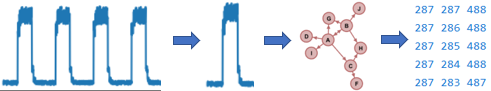
\includegraphics[width=13cm]{fig/tsToNet/tsToCsv}
	\caption{Umwandlung einer Zeitreihe in Netzwerk}
	\label{img:tsToNet}
\end{figure}
\workTodo{Das Netzwerk aus der Grafik noch ab�ndern}



\section{MIDAS}
\label{chap:trsnsMidas}
Die Transformation der Zeitreihe in mehrere Netzwerke funktioniert f�r den MIDAS Algorithmus gleich wie in \autoref{chap:trsnsNeti}. Allerdings kann der Algorithmus teilweise bessere Ergebnisse erzielen, wenn f�r p eine Zahl gr��er als zwei eingesetzt wird. Dadurch werden gr��ere Abst�nde zwischen Elementen st�rker gewichtet.\\
Au�erdem erwartet der MIDAS Algorithmus f�r die Netzwerkdaten ein anderes �bergabeformat. Hierbei k�nnen alle Daten der jeweiligen Zeitabschnitte in einen CSV-File geschrieben werden. Die CSV-Datei muss dabei folgenderma�en strukturiert sein: Ursprungsknoten, Zielknoten, Zeitintervall. Es ist nicht m�glich die Kantengewichtung direkt an den Algorithmus zu �bergeben. Um die Kantengewichtung trotzdem �bergeben zu k�nnen, wird die gleiche Kante mehrmals in Abh�ngigkeit der Gewichtung an den Algorithmus �bergeben.
Wie funkt Midas ganz kurz..


\begin{figure}[H]
	\centering
	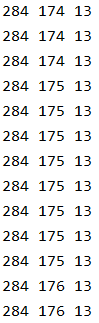
\includegraphics[width=2cm]{fig/tsToNet/midasData}
	\caption{Datensatz Midas}
	\label{img:tsToNetMiData}
\end{figure}


\section{MIDAS-R}
\label{chap:trsnsMidasR}
Der Midas-R Algorithmus speichert weitere Features �ber die Netzwerke. Dazu geh�rt die Gesamtzahl an Kanten, welche von einem Knoten ausgehen und die Aktuelle Anzahl an Kanten die von einem Knoten ausgehen. Aus diesem Grund sind die Berechnungen zur Ausrei�er-Erkennung deutlich umfangreicher. Das Bewirkt, dass die Laufzeit des Algorithmus mit den Daten aus \autoref{chap:trsnsMidas} zu lange ist. Deshalb musste ein L�sung gefunden werden um den Umfang der Daten zu reduzieren, w�hrend die Informationen dennoch erhalten bleiben. Dazu wurde eine Hauptkomponenten Zerlegung durchgef�hrt, welche die Gr��e der Adjazenzmatrix verringert. Der Nachteil hiervon ist das nicht mehr genau gesagt werden kann, welche Kante genau der Ausrei�er ist. 

\workTodo{Midas R liefert eigentlich mehrere Ausrei�er Scores es w�re vielleicht interessant diese einzeln zu betrachten und nicht zusammenaddiert.}
\workTodo{Hab hier das mit der Hauptkomponentenzerlegung gemacht. Wenn es Ergebnisse hierf�r gibt. Kann ich das hier noch erkl�ren}

\newpage
\chapter{Verwendete Datens�tze}

In dieser Ausarbeitung wurden mehrere Datens�tze verwendet, um verschiedene Algorithmen auf ihre Leistungsf�higkeit zu testen. Nachfolgend werden die hierbei verwendeten Datens�tze vorgestellt.

\section*{Numenta-Zeitreihendaten}
\label{sec:numTS}

Der Numenta-Datensatz besteht aus einer Reihe an synthetisch erzeugten Zeitreihen, die unterschiedliche Arten von Ausrei�ern simulieren. Durch die Daten wird es m�glich eine qualitative Aussage �ber die F�higkeiten der Algorithmen zu treffen. F�r die Tests auf multivariaten Zeitreihen wurden neue Zeitreihen erzeugt. Dabei wurde f�r die erste Dimension eine Zeitreihe der Numenta-Gruppe verwendet. F�r h�here Dimensionen wurde auf eine Zeitreihe ohne Ausrei�er zur�ckgegriffen \citep{AHMAD2017134}.

\begin{figure}[H]
	\centering
	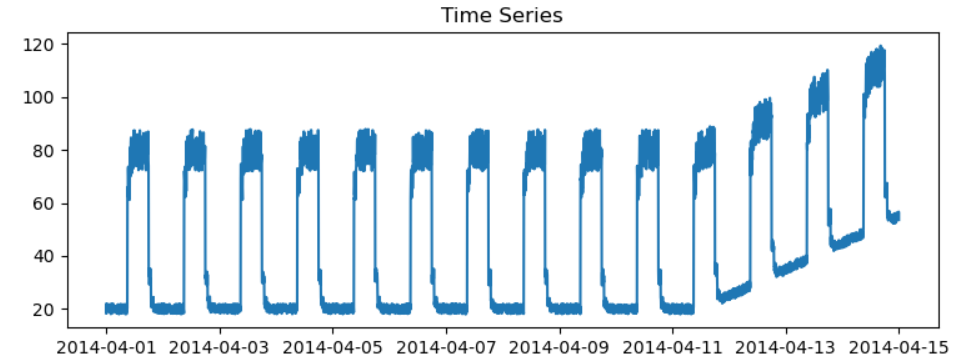
\includegraphics[width=10cm]{fig/numentaExample.PNG}
	\caption{Illustration einer Numenta-Zeitreihe\cite{AHMAD2017134}}
	\label{img:numentaTS}
\end{figure}


\section*{Netzwerk-Datens�tze}
\label{sec:netData}

Zwischen den Forschungsgruppen, welche sich mit der Ausrei�ererkennung in Netzwerken besch�ftigen, herrscht gro�e Konkurrenz. Aus diesem Grund werden gelabelte Datens�tze h�ufig zur�ckgehalten. Dadurch wollen die Forscher verhindern, dass sie ihren Wettbewerbsvorteil gegen�ber anderen verlieren \cite{Problematik}. Aus diesem Grund ist es schwer geeignete Datens�tze zu finden. Mit dem Enron- und Darpa-Datensatz konnten dennoch zwei passende Datens�tze ausgemacht werden. Diese Datens�tze werden im Folgenden vorgestellt.
 
\subsubsection{Enron}



Der Enron Datensatz enth�lt die intern versendeten E-Mail Daten von rund 150 Mitarbeitern der Firma Enron. Die Daten wurden von der Federal Energy Regulatory Commission offengelegt. Enthalten sind ca. 50.000 E-Mail-Nachrichten. F�r den Algorithmus wird lediglich der Zeitpunkt, an dem eine E-Mail versendet wird sowie die Sender und Empf�nger festgehalten.

F�r den Enron Datensatz stehen keine Labels zur Verf�gung. Aus diesem Grund wurden Ausrei�er, die der SedanSpot-Algorithmus gefunden hat, als Labels verwendet. \cite{SedanSpot}. Au�erdem vergleichen die Autoren des SedanSpot-Algorithmus ihre Ausrei�er mit der offiziellen Enron-Zeitleiste. Diese enth�lt ebenfalls Informationen �ber m�gliche historische Gr�nde f�r die Ausrei�er \cite{EnronTimeline}.


\subsubsection{DARPA}

Der DARPA-Datensatz \citep{DARPA} beinhaltet 4.5 Millionen IP-zu-IP-Kommunikationen zwischen 9.400 Quell-IP's und 23.300 Ziel-IP's �ber einen Zeitraum von 87.700 Minuten. Jede Kommunikation ist zu einem Zeitpunkt eine gerichtete Kante von der Quell-IP zur Ziel-IP. Eine vierte Spalte des Datensatzes ist verf�gbar, in der ein \textit{label} enthalten bzw. ein Angriff gekennzeichnet ist. Der DARPA-Datensatz besteht zu �ber 60\% aus Ausrei�ern. 

\newpage
\chapter{Statische Algorithmen zur Ausrei�er Erkennung}
In diesem Kapitel werden zun�chst zwei statische Algorithmen zur Ausrei�er Erkennung auf unterschiedlichen Datentypen (z.B. Videos, Bilder, Netzwerke) vorgestellt. Hierbei handelt es sich um ein auf Percolation basierender Algorithmus und ein auf IsoMap basierender Algorithmus. Statische Algorithmen kennzeichnet, das sie nicht mit Daten umgehen k�nne, welche kontinuierlich an sie �bergeben werden. Damit die Algorithmen anwendbar sind m�ssen die Daten vollst�ndig und abgeschlossen vorliegen. Eines unserer Hauptziele des Forschungsprojektes war die Ausrei�er Erkennung in Zeitreihen, aus diesem Grund untersuchten wir die Algorithmen auf ihre F�higkeit Ausrei�er in Zeitreihen zu finden. In \autoref{sec:IsoBased} wird der Iso Map basierte Algorithmus vorgestellt in \autoref{sec:per-intro} wird der Perculation basierte Algorithmus vorgestellt. 

Beide Algorithmen liefern lediglich einen Ausrei�er Score zur�ck. Um zu bestimmen inwiefern ein Element konkret ein Ausrei�er ist, wird zun�chst den Mittelwert und die Standardabweichung des Outlier Scores berechnet. Falls ein Element in Abh�ngigkeit von der Standardabweichung sehr stark vom Mittelwert abweicht wird das Element als Ausrei�er klassifiziert.

\section{Umwandlung Zeitreihe in Netzwerk}

Damit sowohl der auf Perculation basierende Algorithmus wie auch der auf Iso Map basierende Algorithmus angewandt werden k�nnen, m�ssen die Daten zun�chst in ein einheitliches Format �berf�hrt werden. Dazu m�ssen die unterschiedlichen Daten in ein Netzwerk umgewandelt werden.  Hierzu ist erforderlich, dass eine Distanz zwischen unterschiedlichen Elementen des Datensatzes berechnet werden kann  \citep[vgl.][S.~2]{10.3389/fphy.2019.00194}. Der Algorithmus kann auf allen Daten angewandt werden, welche diese Vorraussetzung erf�llen. Nachfolgend wird exemplarisch beschrieben wie die Transformation f�r eine Zeitreihe funktionieren kann. 


\label{sec:trsnsNeti}
F�r die Transformation der Zeitreihe, muss zun�chst die Distanz zwischen den einzelnen Elementen (Zeitpunkten) der Zeitreihe berechnet werden. Hierzu wird das Distanzma� aus  \autoref{eq:euklidianDist} genutzt. 

\begin{equation}
	D_{ij}=\left(\sum_{k} \left|v_{k}^{i}-v_{k}^{j}\right|^{p}\right)^{1/p} \label{eq:euklidianDist}
\end{equation}

Insofern in die Gleichung f�r p = 2 eingesetzt wird, handelt es sich hierbei um die euklidische Distanz. Die mit \autoref{eq:euklidianDist} berechneten Distanzen bilden die Kantengewichte in dem neu erstellten Netzwerk. Das neue Netzwerk ist hierbei Fully Connected. Das hei�t jeder Knoten ist mit allen anderen Knoten �ber eine Kante verkn�pft. Die Knoten des Netzwerks repr�sentieren die einzelnen ELemente(Zeitpunkte) der zeit reihe. \citep[vgl.][S.~2]{10.3389/fphy.2019.00194}. Es k�nnen mit dieser Vorgehenswei�e auch multivariate Zeitreihen in ein Netzwerk transformiert werden.


\section{IsoMap Basierter Algorithmus}
\label{sec:IsoBased}
Der Ansatz dieses Algorithmus ist, dass Informationen �ber Ausrei�er bei der Reduzierung der Dimensionalit�t mit dem IsoMap verloren gehen. Insofern versucht wird, die Informationen zu rekonstruieren und mit der urspr�nglichen Matrix vergleicht, k�nnen gro�e Abweichungen bei Ausrei�er Elementen festgestellt werden \citep[vgl.][S.~3]{10.3389/fphy.2019.00194}. In \autoref{ssec:iso-algo} wird zun�chst erkl�rt wie der Iso Map Algorithmus eine Reduzierung der Dimensionalit�t durchf�hrt. Anschlie�end werden in \autoref{ssec:iso-weiter} die zus�tzlichen Schritte erl�utert, welche notwendig sind um Ausrei�er mithilfe des IsoMap Algorithmus zu erkennen.


\subsection{IsoMap}
\label{ssec:iso-algo}
Beim IsoMap handelt es sich um einen Algorithmus zur nichtlinearen Dimensionsreduktion. Zun�chst werden beim IsoMap Algorithmus die Nachbarn eines jeden Punktes(Knoten) �ber K-Nearest Neighbor bestimmt. Anschlie�end wird jeder Punkt mit den gefundenen Nachbarn verkn�pft, wodurch ein neuer K�rper(Netzwerk) entsteht. Daraufhin wird eine neue Distanzmatrix auf dem entstandenen K�rper berechnet, indem die k�rzeste Distanz zwischen allen Punkten auf dem K�rper berechnet wird. Diese Matrix kann auch als geod�tische Distanzmatrix $D_{G}$ bezeichnet werden. Die eigentliche Dimensionsreduktion wird anschlie�end �ber die Eigenvektoren und Eigenwerte der Matrix $D_{G}$ durchgef�hrt. Das Ergebnis der Dimensionsreduktion ist eine neue Menge an Features f�r jedes Element $V^{i} = {v^{i}_{1}. . . v^{i}_{r}}$ des urspr�nglichen Datensatzes. Durch das Erzeugen der Matrix $D_{G}$ wird erreicht, das nichtlineare Zusammenh�nge bei der Dimensionsreduktion erhalten bleiben. \citep[vgl.][S.~3-4]{Tenenbaum2319}.

\begin{figure}[H]
	\centering
	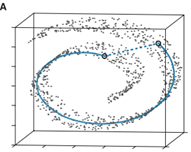
\includegraphics[width=5cm]{fig/isomap_circle.png}
	\caption{Berechnung der Distanz zwischen zwei Punkten nach Anwendung des IsoMap Algorithmus}
	\label{img:isomap}
\end{figure}


\subsection{IsoMap zur Erkennung von Ausreisern}
\label{ssec:iso-weiter}
Mithilfe des IsoMap Algorithmus wurden f�r jedes Element neue Features ($V^{i} = {v^{i}_{1}. . . v^{i}_{r}}$) berechnet. Im n�chsten Schritt wird versucht aus diesen Featurn die urspr�ngliche Distanzmatrix zu rekonstruieren. Dazu wird aus den Featuren $V^{i}$ unter Verwendung von \autoref{eq:euklidianDist} eine neue Distanzmatrix $\hat{D}$ berechnet. Nun k�nnen die Matrizen $D_{G}$ und $\hat{D}$ miteinander verglichen werden. Hierzu muss die Pearson Korrelation zwischen den jeweiligen Spalten der Matrizen berechnet werden. F�r Ausrei�er wird erwartet, dass die Korrelation sehr niedrig ist, da Informationen �ber sie bei der Reduktion verloren gehen \citep[vgl.][S.~3]{10.3389/fphy.2019.00194}.

\subsection{Implementierung}
\label{sec:im-implement}
F�r den Iso Map Algorithmus stellt SciKit Learn eine sehr gute Implementierung zur Verf�gung. Diese Implementierung konnten wir gut in unseren Algorithmus integrieren. Es musste lediglich ge�ndert werden, dass auf die Matrix $D_{G}$ zugegriffen werden kann. Dies ist standardm��ig nicht der Fall. F�r die Implementierung der weiteren Funktionalit�t wurde auf Python/Numpy zur�ckgegriffen. 

\subsection{Ausrei�ererkennung in Zeitreihen}
\workTodo{Erkl�ren welche Zeitreihen verwendet wurden. Hab ich so ein bisschen gemacht vielleicht das noch in extra Kapitel machen.} 
\label{sec:im-results}
\begin{table}
\caption{IsoMap Performance}
\begin{tabular}{ |p{4.5cm}||p{4.5cm}||p{3cm}|}
	\hline
	\textbf{Ausrei�er Typ}& \textbf{Datei Name}&
	\textbf{1D}\\
	\hline
	\hline
	Einzelne Peaks & anomaly-art-daily-peaks & *\\
	\hline
	Zunahme an Rauschen & anomaly-art-daily-increase-noise &**\\
	\hline
	Signal Drift & anomaly-art-daily-drift &**\\
	\hline
	Kontinuierliche Zunahme der Amplitude& art-daily-amp-rise & **\\
	\hline
	Zyklus mit h�herer Amplitude & art-daily-jumpsup &*\\
	\hline
	Zyklus mit geringerer Amplitude & art-daily-jumpsdown & **\\
	\hline
	Zyklus-Aussetzer & art-daily-flatmiddle &*\\
	\hline
	Signal-Aussetzer & art-daily-nojump & -\\
	\hline
	Frequenz�nderung & anomaly-art-daily-sequence-change &-\\
	\hline
\end{tabular}
\end{table}

F�r die durchgef�hrten Tests wurden die Zeitreihen aus ... verwendet. Um zu bewerten wie gut der Algorithmus funktioniert, wurde ein Punktesystem eingef�hrt. In dem Punktesystem konnten maximal vier Sterne erreicht werden. Das bedeutet Ausrei�er sehr gut erkannt. Null Sterne hingegen bedeuten Ausrei�er �berhaupt nicht erkannt. Der IsoMap Algorithmus liefert eher schwache Ergebnisse bei der Erkennung von Ausrei�ern in Zeitreihen. Hauptproblem hierbei ist, dass starke Anstiege, bei welchen es sich nicht um Ausrei�er handelt, f�lschlicherweise zu einem starken Anstieg des Ausrei�er Scores f�hren (vgl. \autoref{img:iso_trans} mit Pfeil markierte stellen). Dies kann, je nach Threshold, zu einer hohen Quote an falsch positiven Klassifizierungen f�hren. Aus diesem Grund k�nnen die tats�chlichen Ausrei�er nicht eindeutig identifiziert werden. Eine �hnliche Problematik trat in \citep {Uzun} bei der Verwendung des Random Walk Algorithmus auf. Das Problem konnte hierbei gel�st werden, indem vor der Anwendung des Algorithmus, eine Gl�ttung der Zeitreihe durchgef�hrt wurde. Dadurch werden abrupte �bergange in der Zeitreihe abgemildert und deshalb nicht mehr als Ausrei�er erkannt \citep[vgl.][S.~31,36]{Uzun}. Dies k�nnte ein m�glicher Ansatz sein um zuk�nftig bessere Ergebnisse zu erzielen.\\
Des Weiteren ist zu erkennen, dass der Algorithmus f�r einige Ausrei�er Typen nicht geeignet ist, hierzu geh�ren Siganl Aussetzer und Frequenz�nderungen. Bei diesen Ausrei�er Typen treten keinerlei un�blichen Werte auf, sondern es kommt zu �nderungen in der Saisonalit�t der Zeitreihe. 

\workTodo{Wie genau bezieht man sich auf seine eigene Ausarbeitung} 

\begin{figure}[H]
	\centering
	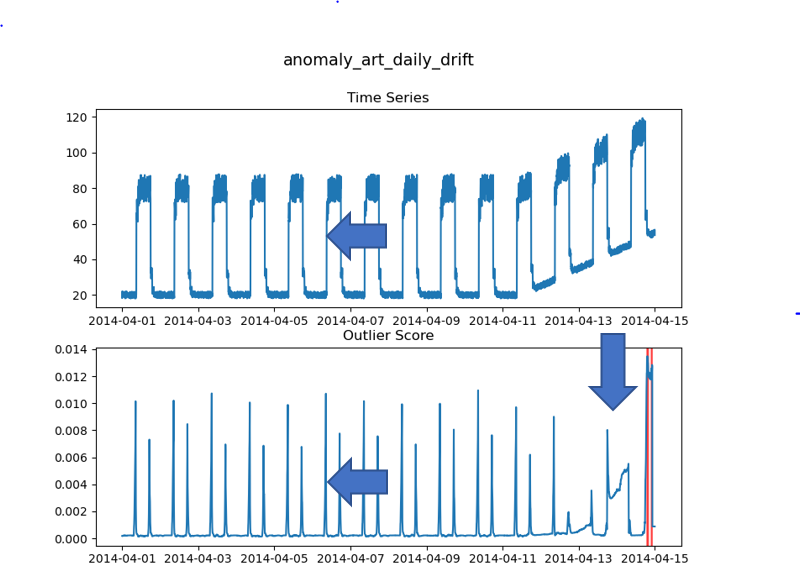
\includegraphics[width=10cm]{fig/resultsIsoMap/problem_transitions.PNG}
	\caption{Problem �berg�nge}
	\label{img:iso_trans}
\end{figure}


\newpage
\section{Perculation basierter Algorithmus}
\label{sec:per-intro}
Bei diesem Algorithmus werden schrittweise die Kanten mit den h�chsten Gewichten aus der mit \autoref{eq:euklidianDist} erzeugten Distanzmatrix $D_{ij}$ entfernt. Ziel dieses Prozesses ist es Ausrei�er vom restlichen Teil des Netzwerks zu trennen. Dabei kann davon ausgegangen werden, dass Ausrei�er h�here Kantengewichte zu ihren Nachbarn aufweisen und deshalb schneller separiert werden. Sobald ein Knoten komplett separiert ist, wird ihm ein Ausrei�er Score zugeordnet. Der Wert des Ausrei�er Scores wird �ber die zuletzt entfernte Kante des Knoten definiert. Dadurch erhalten fr�her separierte Knoten h�here Ausrei�er Scores als sp�ter separierte Knoten \citep[vgl.][S.~3]{10.3389/fphy.2019.00194}. 

\begin{figure}[H]
	\centering
	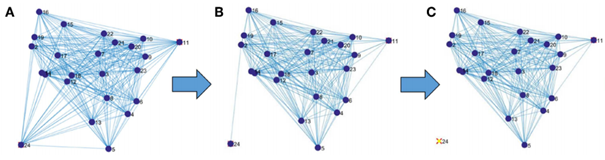
\includegraphics[width=15cm]{fig/perco_procedure.png}
	\caption{Ablauf Perculation basierter Algorithmus}
	\label{img:perc_proc}
\end{figure}

\subsection{Implementierung}
\label{sec:per-imp}
F�r die Implementierung des Perculation-basierten Algorithmus wurde genauso wie in \autoref{sec:im-implement}, Python/Numpy verwendet. Bei der Implementierung eines Prototypen des Algorithmus konnte festgestellt werden, das die Laufzeit des Algorithmus sehr langsam ist. Aus diesem Grund wurden einige Ver�nderungen an dem Algorithmus vorgenommen um die Performance zu verbessern. Dazu geh�rte, dass nicht einzelne Kanten, sondern Gruppen an Kanten aus dem Netzwerk entfernt werden. Der Vorteil dieser Modifikation ist, dass seltener �berpr�ft werden muss ob ein Knoten weiterhin mit den Rest des Netzwerks verbunden ist. Eine weitere Verbesserung, die eingef�hrt wurde, ist die Verankerung eines Abbruchkriteriums. Dabei wird der Algorithmus angehalten sobald 
eine bestimmte Menge an Kanten aus dem Netzwerk entfernt wurde. Da der Algorithmus nicht alle Berechnungen ausf�hren muss, kann damit eine Optimierung der Laufzeit erreicht werden. Weiterhin konnte festgestellt werden, dass diese Ver�nderung keinen Einfluss auf die Qualit�t der Ausrei�er Erkennung hat, da Ausrei�er lediglich zu Beginn des Algorithmus gefunden werden. Ein weiteres Problem des Urspr�nglichen Algorithmus war, das bei aufeinanderfolgenden Elemente der Zeitreihe teilwei�e starke Schwankungen im Ausrei�er Score auftraten (vgl. \autoref{img:vardir1}). Aus diesem Grund konnten Ausrei�er, welche sich �ber mehrere Zeitpunkte hinweg erstrecken nicht komplett erkannt werden. Um die Schwankungen im Ausrei�er Score abzumildern, wurde dieser gegl�ttet. Dazu wurde der Gleitende Mittelwert des Ausrei�er Scores berechnet. In \autoref{eq:slidingAverage} ist exemplarisch die Formel f�r einen Gleitenden Mittelwert der Ordnung drei dargestellt. In \autoref{img:vardir1} ist zu sehen wie sich der Ausrei�er Score durch das Gl�tten ver�ndert. 
\begin{equation}
	m_{\text{MA}}^{(3)}(t)={\frac {1}{3}}{\Big (}x(t-1)+x(t)+x(t+1){\Big )} \label{}
\end{equation} 

\workTodo{Das Verfahren zur Gl�ttung das hier eingesetzt wird hei�t gleitender Mittelwert. Vielleicht FOrmel davon einf�gen und dan noch passende Quelle finden}
\workTodo{Parameter noch erkl�ren} 
\begin{figure}[h]
	\centering
	\subfloat{
		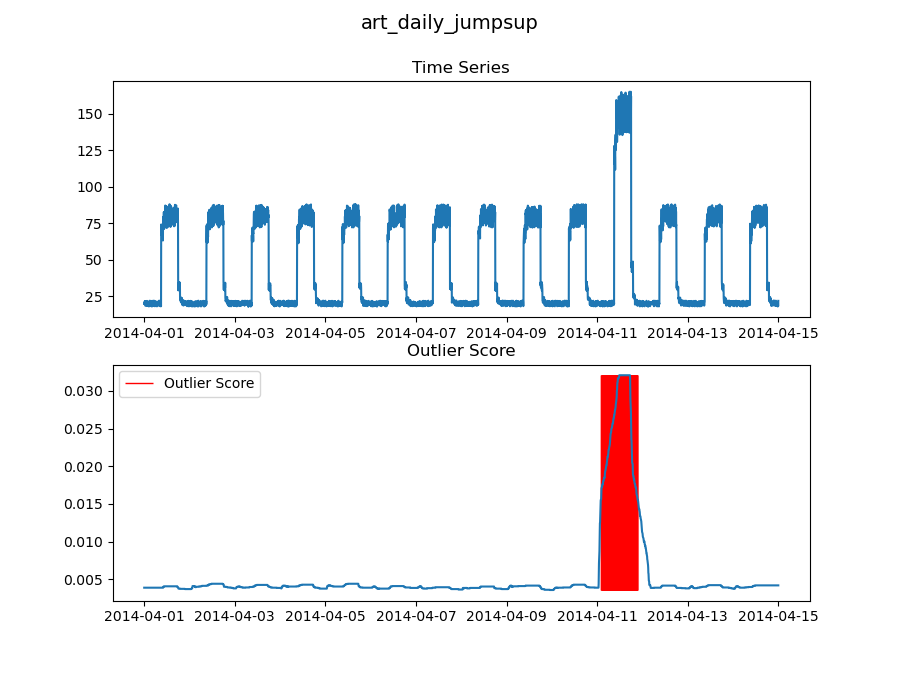
\includegraphics[width=0.5\textwidth]{fig/resultsPercolation/art_daily_jumpsup}}
	\subfloat{
		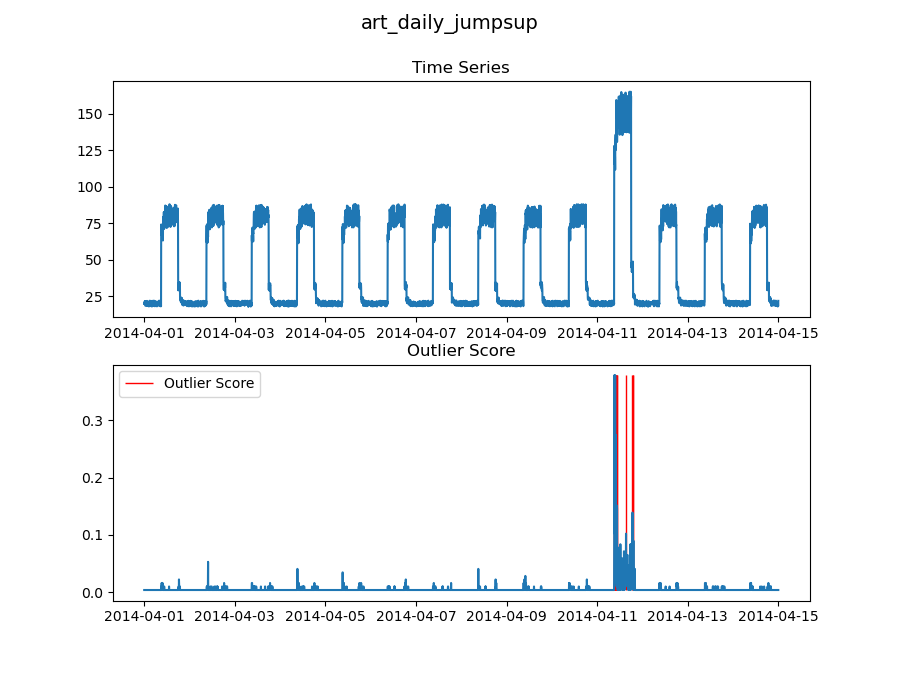
\includegraphics[width=0.5\textwidth]{fig/resultsPercolation/art_daily_jumpsup_ohne}}
	\caption{Vergelich Perculation Algorithmus mit Sliding Window Verfahren und ohne Sliding Window Verfahren}
	\label{img:vardir1}
\end{figure}

\subsection{Ausrei�ererkennung in Zeitreihen}
\label{sec:per-result}

\begin{table}
\caption{Perculation Time Series Performance}
\begin{tabular}{ |p{6cm}||p{6cm}||p{3cm}|}
	\hline
	\textbf{Ausrei�er Typ}& \textbf{Datei Name}&
	\textbf{1D}\\
	\hline
	\hline
	Einzelne Peaks & anomaly-art-daily-peaks & *\\
	\hline
	Zunahme an Rauschen & anomaly-art-daily-increase-noise &****\\
	\hline
	Signal Drift & anomaly-art-daily-drift &***\\
	\hline
	Kontinuierliche Zunahme der Amplitude& art-daily-amp-rise & ***\\
	\hline
	Zyklus mit h�herer Amplitude & art-daily-jumpsup &****\\
	\hline
	Zyklus mit geringerer Amplitude & art-daily-jumpsdown & ****\\
	\hline
	Zyklus-Aussetzer & art-daily-flatmiddle &****\\
	\hline
	Signal-Aussetzer & art-daily-nojump & -\\
	\hline
	Frequenz�nderung & anomaly-art-daily-sequence-change &-\\
	\hline
\end{tabular}
\end{table}

\label{sec:per-results-text}
Es konnte festgestellt werden, dass der Perculation basierte Algorithmus, viele Ausrei�er Typen sehr gut erkennt. Ob Ausrei�er in einer Zeitreihe mit einzelnen Peaks gefunden werden, h�ngt davon ab, ob der Ausrei�er Score gegl�ttet wird. Insofern keine Gl�ttung des Ausrei�er Scores durchgef�hrt wird, k�nnen einzelne Peaks gefunden werden. Denn durch die Gl�ttung der Zeitreihe verschwinden die Ausschl�ge im Ausrei�er Score. Es muss also in Abh�ngigkeit des Anwendungsfalles entschieden werden ob der Ausrei�er Score gegl�ttet wird. Dabei w�re ebenfalls denkbar, das beide Varianten zur Erkennung von Ausrei�ern verwendet werden. Der Perculation basierte Algorithmus ist genauso wie der Iso Map basierte Algorithmus (vgl. \autoref{sec:im-results}) nicht dazu im Stande Ausrei�er in Zeitreihen mit Signal Aussetzer und Frequenz�nderung zu erkennen.   

\newpage
\chapter{Dynamische Algorithmen zur Ausrei�ererkennung}
\label{chap:dynamic}

In diesem Kapitel werden zwei Algorithmen zur dynamischen Erkennung von Ausrei�ern vorgestellt. Hierbei handelt es sich um den NetSimile- (vgl. \autoref{sec:ns}) und den MIDAS- (vgl. \autoref{sec:midas}) Algorithmus. Dynamische Algorithmen k�nnen im Gegensatz zu statischen Algorithmen, Ausrei�er in Echtzeitdaten finden. Dies kann in der Praxis sehr wichtig sein, da Ausrei�er m�glichst schnell gefunden werden m�ssen, um die daraus resultierenden finanzielle Sch�den abzuwenden.  Im Zuge des Forschungsprojekts werden die dynamischen Algorithmen ebenfalls auf den unterschiedlichen Input, der sich aus den verschiedenen Anwendungsf�lle ergibt, angepasst. Dadurch wird gew�hrleistet, dass diese Algorithmen, ebenso wie die statischen Algorithmen aus \autoref{chap:static}, mit unterschiedlichen Datentypen umgehen k�nnen. In den Tests des Forschungsprojekts werden die Algorithmen auf Netzwerk- und Zeitreihendaten angewendet.

\section{Umwandlung der Daten in einen Graphen}

Bevor die dynamischen Algorithmen auf die Zeitreihendaten angewendet werden k�nnen, m�ssen diese in Graphen transformiert werden. Dabei funktioniert die Umwandlung der Daten �hnlich wie bei statischen Algorithmen (vgl. \autoref{sec:trsnsStatic}). Der einzige Unterschied ist der, dass jeweils schrittweise kleine Abschnitte der Daten in Graphen umgewandelt werden. Nachfolgend wird dies an einem Beispiel n�her veranschaulicht. Ein Temperatursensor liefert jede Sekunde einen Wert. Sobald 100 Werte des Sensors eingegangen sind, erfolgt die Umwandlung dieser Daten in einen Graphen unter Verwendung von \autoref{eq:euklidianDist}. Dieser Vorgang wiederholt sich anschlie�end immer wieder. Der Wert f�r die L�nge der Abschnitte ist hierbei frei w�hlbar und kann als Parameter �bergeben werden. Insofern die Zeitreihe eine Saisonalit�t besitzt, bietet es sich an diese f�r die L�nge der Abschnitte zu verwenden. In einem letzten Schritt werden anschlie�end die Netzwerkdaten in eine Datei geschrieben. Dieser Schritt ist aufgrund der Art und Weise, wie die Algorithmen implementiert sind notwendig. In \autoref{img:tsToNet} ist graphisch dargestellt wie die Umwandlung der Daten in ein Netzwerk funktioniert. 

\begin{figure}[H]
	\centering
	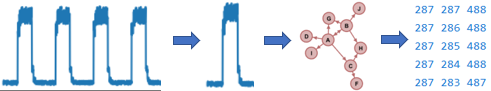
\includegraphics[width=13cm]{fig/tsToNet/tsToCsv}
	\caption{Umwandlung einer Zeitreihe in einen Beispielgraphen.}
	\label{img:tsToNet}
\end{figure}

\label{ssec:trsnsCSV}
Die verschiedenen Algorithmen erfordern unterschiedliche �bergabeformate. Aus diesem Grund werden anschlie�end kurz die Besonderheiten erkl�rt, auf welche dabei geachtet werden muss. \\

\begin{mldescription}
	\mlitem{NetSimile:} Das �bergabeformat f�r den NetSimile-Algorithmus ist in \autoref{img:tsToNet} ganz rechts dargestellt. Jede Zeile stellt hierbei eine Kante des Netzwerks dar. Bei der ersten Spalte handelt es sich um den Ursprungsknoten der Kante, bei der zweiten Spalte um den Zielknoten und bei der letzten Spalte um die Gewichtung.
	\mlitem{MIDAS:}  Beim MIDAS-Algorithmus ist es nicht m�glich die Gewichtung der Kanten direkt an den Algorithmus zu �bergeben. Es ist jedoch m�glich die Gewichtung der Kanten indirekt an den Algorithmus zu �bergeben, indem gleiche Kanten mehrmals in Abh�ngigkeit der Gewichtung an den Algorithmus �bergeben. In \autoref{img:tsToNetMiData} ist ein kleiner Ausschnitt einer Datei f�r den MIDAS dargestellt.
	\mlitem{MIDAS-R:} Die Berechnungen f�r den MIDAS-R Algorithmus sind im Verh�ltnis zum MIDAS Algorithmus umfangreicher. Insofern f�r den MIDAS-R Algorithmus die gleichen Daten verwendet werden wie f�r den MIDAS Algorithmus, ben�tigen die Berechnungen sehr lange. Aus diesem Grund wurde eine Hauptkomponenten Zerlegung durchgef�hrt, um die Gr��e der Adjazenzmatrix zu verringert. Es entsteht ein kleineres Netzwerk, welches an den MIDAS-R Algorithmus �bergeben werden kann. \label{ssec:trsnsMidasR}
\end{mldescription}

\begin{figure}[H]
	\centering
	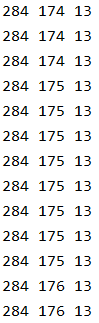
\includegraphics[width=2cm]{fig/tsToNet/midasData}
	\caption{Datensatz f�r MIDAS bestehend aus Ursprungsknoten, Zielknoten und Zeitabschnitt}
	\label{img:tsToNetMiData}
\end{figure}

\newpage
\section{Netsimile}
\label{sec:ns}

\subsection{Grundlagen}
\label{ssec:ns-gl}

Netsimile ist ein skalierbarer Algorithmus zur Erkennung von �hnlichkeiten, sowie Anomalien in Netzwerken unterschiedlicher Gr��en. Hierf�r wird der Datensatz in gleich gro�e Zeitintervalle unterteilt, um die daraus resultierenden Graphen auf unterschiedliche Merkmale zu untersuchen. Die Merkmale sind hierbei strukturelle Eigenschaften der einzelnen Knoten wie bspw. die Dichte eines Knotens oder die Anzahl an Nachbarn in einem Ego-Netzwerk. Die Signatur ergibt sich aus den einzelnen Aggregationen der Knoten wie bspw. der Median aus der Dichte der jeweiligen Knoten. So entsteht bspw. aus sieben Merkmalen und f�nf Aggregationen ein Signaturvektor mit 35 verschiedenen Signaturen. So erm�glicht der Signarturvektor die Beschreibung als auch den Vergleich der einzelnen Graphen. F�r den Vergleich wird die Canberra Distanz aus den beiden Signaturvektoren zweier zeitlich nebeneinander liegenden Graphen berechnet. \citep[vgl.][S.~1]{Netsimile}

Als Input f�r diesen Algorithmus wird eine Menge von $k$-anonymisierten Netzwerken mit beliebig unterschiedlichen Gr��en, die keine �berlappenden Knoten oder Kanten besitzen sollten, herangezogen werden. Das Resultat sind Werte f�r die strukturelle �hnlichkeit oder Abstands eines jeden Paares der gegebenen Netzwerke bzw. ein Merkmalsvektor f�r jedes Netzwerk. \citep[vgl.][S.~1]{Netsimile}

Netsimile durchl�uft drei Schritte, die im Folgenden erl�utert werden.

\subsubsection{Extrahierung von Merkmalen}
F�r jeden Knoten $i$ werden, basierend auf ihren Ego-Netzwerken, die folgenden Merkmale generiert:


\begin{description}
	\item[$\overline{d}_i = |N(i)|$]\hfill\\ Die Anzahl der Nachbarn (d.h. Grad) von Knoten $i$, wobei $N(i)$ die Nachbarn von Knoten $i$ beschreibt.
	\item[$\overline{c}_i$]\hfill\\ Der Clustering-Koeffizient von Knoten $i$, der als die Anzahl von Dreiecken, die mit Knoten $i$ verbunden sind, �ber die Anzahl von verbundenen Dreiecken, die auf Knoten $i$ zentriert sind, definiert ist.
	\item[$d_{N(i)}$]\hfill\\ Die durchschnittliche Anzahl der Nachbarn von Knoten $i$, die zwei Schritte entfernt sind. Dieser wird berechnet als \workTodo{Paper Seite 2 unten Formel einf�gen}
	\item[$c_{N(i)}$]\hfill\\ Der durchschnittliche Clustering-Koeffizient von $N(i)$, der als \workTodo{Paper Seite 2 unten Formel einf�gen} berechnet wird.
	\item[$|E_{ego(i)}|$]\hfill\\ Die Anzahl der Kanten im Ego-Netzwerk vom Knoten $i$, wobei $ego(i)$ das Ego-Netzwerk von $i$ zur�ckgibt.
	\item[$|E^{\circ}_{ego(i)}|$]\hfill\\ Die Anzahl der von $ego(i)$ ausgehenden Kanten. 
	\item[$|N(ego(i))|$]\hfill\\ Die Anzahl von Nachbarn von $ego(i)$. 
\end{description}

\subsubsection{Aggregierung von Merkmalen}
Im n�chsten Schritt wird f�r jeden Graphen \textit{$G_j$} eine $Knoten \times Merkmal$-Matrix $F_{G_j}$ zusammengefasst. Dieser besteht aus den Merkmalsvektoren aus Schritt 1.
Da der Vergleich von $k$-ten $F_{G_j}$ sehr aufw�ndig ist, wird f�r jede $F_{G_j}$ ein Signaturvektor $\vec{s}_{G_j}$ ausgegeben. Dieser aggregiert den Median, den Mittelwert, die Standardabweichung, die Schiefe, sowie die Kurtosis der Merkmale aus der Matrix.  

\subsubsection{Vergleich der Signaturvektoren}
\label{sec:ns-gl-cd}

F�r die Ausrei�ererkennung werden die letzten drei Graphen anhand der Canberra-Distanz-Funktion, die als �hnlichkeitsma� dient, herangezogen. Steigt die Canberra Distanz zwischen zwei Graphen oberhalb des Thresholds so wird dies im Algorithmus festgehalten. Falls der darauf folgende Graph ebenfalls oberhalb des Thresholds liegt, so wird dieser als Ausrei�er definiert. Dadurch wird die Anzahl der Ausrei�er reduziert, damit nur diejenigen identifiziert werden, bei denen ein Trend hin zu einem abnormalen Verhalten erkennbar ist.

Der Algorithmus arbeitet dabei dynamisch, da die Signaturen der Graphen in einzelne Teil-Berechnungen aufgesplittet und zwischengespeichert werden k�nnen, ohne das eine Neuberechnung notwendig ist. Der Threshold wird aus dem Median und dem Mean berechnet, welche ebenfalls Zwischengespeichert werden k�nnen und nach Bedarf um weitere Graphen erg�nzt werden k�nnen.

\FloatBarrier

\subsection{Anwendung des Algorithmus auf Netzwerkdaten}
\label{sec:ns-ext}
Beim ersten Versuch den Algorithmus auf Netzwerkdaten anzuwenden, wurde folgende Probleme festgestellt:

Der Algorithmus verwendet eine Bibliothek \textit{igraph}, welche Kanten zwischen zwei Knoten nur einmalig hinzuf�gen kann. Beim Eliminieren der Duplikate w�rde aber ein Drittel des Datensatzes nicht ber�cksichtigt werden, wodurch wertvolle Informationen bei der Ausrei�ererkennung verloren gehen w�rden. Aus diesem Grund wurden die Netzwerkdaten soweit angepasst, dass Mehrfachverbindungen zwischen zwei Kanten aufsummiert werden und als Gewichtung dieser Kante hinzugef�gt wird. 

\begin{lstlisting}[language=Python, caption=Gewichtung als neues Feature, label=lst:netsimile:code1]
for i in range(len(e_list)): 
	g.add_edge(e_list[i][0], e_list[i][1], weight=e_list[i][2])
\end{lstlisting}

Dadurch kann der Datensatz zum einen vollst�ndig analysiert werde und zum anderen konnte dadurch ein weiteres Feature hinzugef�gt werden, dass durch die f�nf verschiedenen Aggregationen den Signaturvektor um diese f�nf Werte erweitert.

Dadurch das der Datensatz zuerst eingelesen und in einen Graphen transformiert wird und anschlie�end aus dem Graphen die jeweiligen Features extrahiert werden, verliert der Algorithmus extrem an Performanz. Des weiteren wird im ersten Schritt der maximale Knoten-Wert als Gr��e des Graphens �bergeben. Wird bspw. f�r jeden Mitarbeiter eine eigene ID �bergeben und die inkrementell erh�ht, so kann es sein, dass aus einem Netzwerk mit 20 verschiedenen Knoten ein Graph erzeugt wird, der 1000 Knoten erzeugt, weil eine ID mit dem Wert 1000 vorhanden ist. Dadurch b��t die Performanz an Geschwindigkeit ein, da Iterationen nicht �ber die 20 Knoten durchgef�hrt werden, sondern �ber 1000. Hier muss entweder der Datensatz vorab angepasst werden, indem die IDs neu vergeben werden oder der Algorithmus muss grundlegend neu aufgebaut werden.

Da der Fokus auf der Anwendung von Zeitreihen liegt, wird die Optimierung erst in diesem Abschnitt erl�utert.



Das Problem hierbei ist, dass jeder Knoten eines Graphens die gleichen Features beinhalten w�rde. Dadurch w�rden die Aggregationen �berfl�ssig werden und der Signaturvektor auf sieben Features schrumpfen. Die Bildung von Cluster-Features w�re demnach nur noch bedingt m�glich und die Betrachtung an Nachbarn, unabh�ngig ob im Ego-Netzwerk oder im gesamten Netzwerk w�rde sich die Gesamtanzahl an Knoten ann�hern. Im Folgenden wird das Verh�ltnis der Features zum Durchschnitt dargestellt.

\subsubsection{Anwendung auf ENRON-Datensatz}
\label{sec:ns-enron}

Da der Enron Datensatz ebenfalls von einem anderen Paper analysiert und ver�ffentlicht wurde, k�nnen die dort erkannten Ausrei�er zum Vergleich in Form eines gelabelten Datensatz verwendet werden.
Betrachtet man in diesem Kontext den Aurei�erscore, ist gut zu erkennen, dass der Ausrei�er Ende 2001 als alleiniger herausstechender Ausrei�er auch im Ergebnis wiederzufinden ist. Grundlegend ist aber auch zu erkennen, dass die Ausrei�er sich nur sehr wenig voneinander unterscheiden, wodurch eine Klassifizierung innerhalb des Ausrei�erscores sich als schwierig erweist. Die Extrahierung weiterer Features k�nnte hier eventuell aushelfen, wobei dies nicht im Rahmen dieses Forschungsprojektes behandelt werden soll, da der Fokus auf Zeitreihen liegt. Zwecks Performanz konnte der Datensatz innerhalb von zwei Minuten analysiert werden.

\begin{figure}[H]
	\centering
	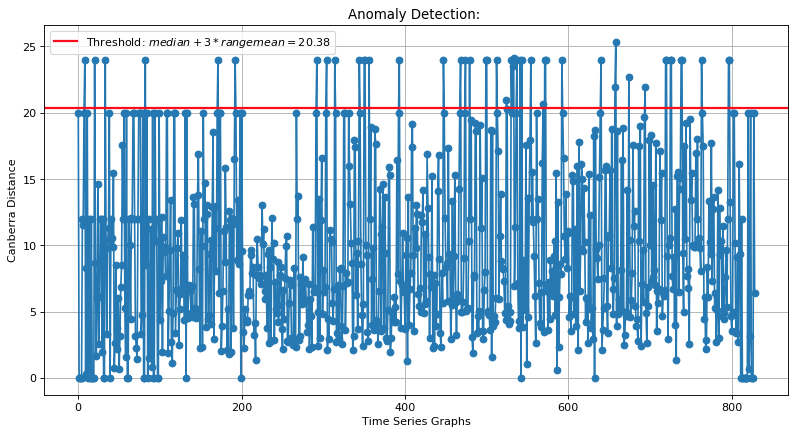
\includegraphics[height=0.6\linewidth,width=\linewidth]{fig/netsimile/anomalie_3}
	\caption{Ausrei�er Score Enron Datensatz}
	\label{img:netsimile:anomalie_3}
\end{figure}

\begin{figure}[H]
	\centering
	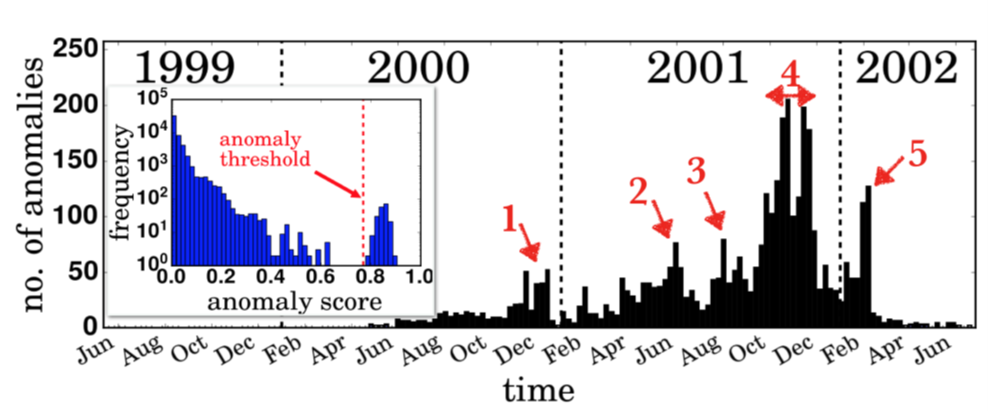
\includegraphics[height=0.6\linewidth,width=\linewidth]{fig/sedanspot}
	\caption{\workTodo{Sedanspot Caption}}
	\label{img:sedanspot}
\end{figure}

Betrachtet man die Differenz aus dem Durchschnitt der Signaturvektoren und den der Ausrei�ergraphen in einer Headmap kann man erkennen, dass die Ausrei�er vorwiegend durch besonders gro�e Ego-Netzwerke und einer hohen Anzahl an E-Mails verschuldet ist.



\begin{figure}[H]
	\centering
	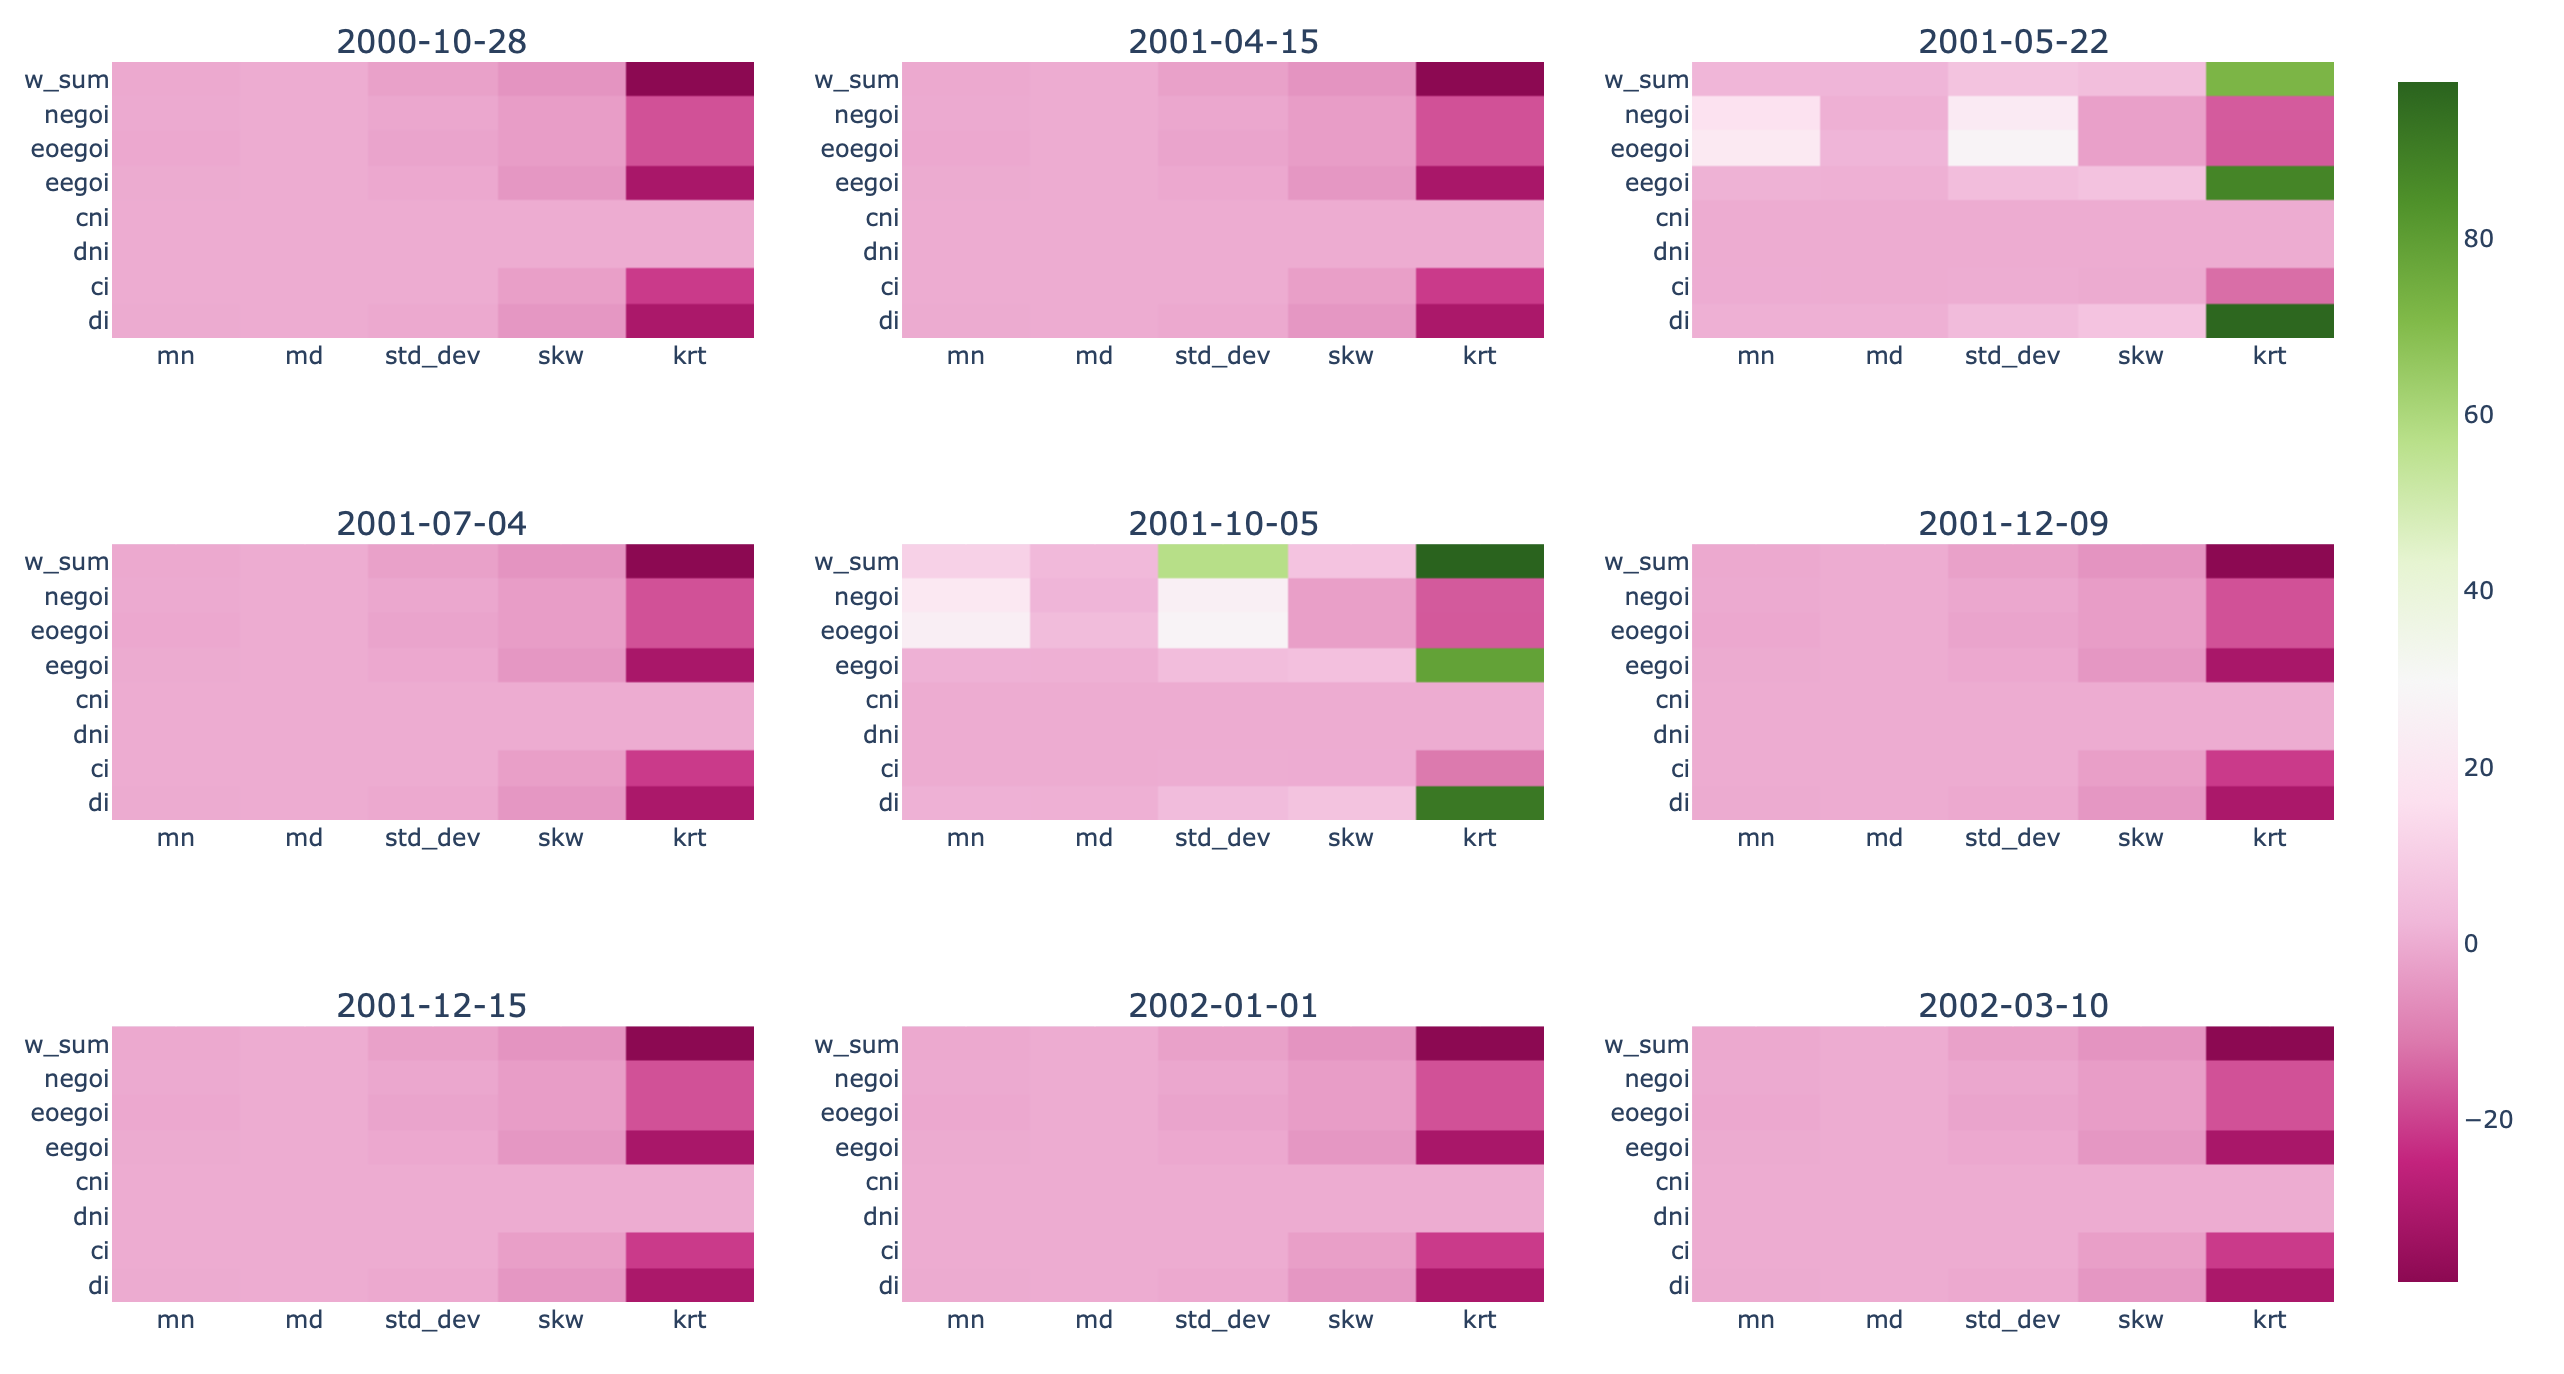
\includegraphics[height=0.8\linewidth,width=\linewidth]{fig/netsimile/heatmap_3}
	\caption{Darstellung der Ausrei�er in Heatmaps}
	\label{img:netsimile:heatmap_3}
\end{figure}

\subsubsection{Anwendung auf DARPA-Datensatz}
\label{sec:ns-darpa}

Beim Darpa Datensatz k�nnen die Aurei�er besser klassifiziert werden. Die Gr�nde k�nnen hierbei auf die Gr��e und Vielfalt des Datensatzes zur�ckgef�hrt werden. Der Enron Datensatz hat eine Gr��e von 1MB und rund 50.000 Kanten. Der Darpa Datensatz hingegen hat eine Gr��e von 50 MB mit 4.5 Mio Kanten. Die Berechnung hat dabei eine L�nge von 3h. Haben wir bei der Dateigr��e den Faktor 50 und bei der Kantenanzahl den Faktor 90, so ist bei der Berechnungszeit der Faktor 90 wiederzufinden. Betrachtet man die Laufzeit, so kann eine lineare Abh�ngigkeit zwischen Kantenanzahl und der ben�tigten Berechnungszeit festgestellt werden.

\begin{figure}[H]
	\centering
	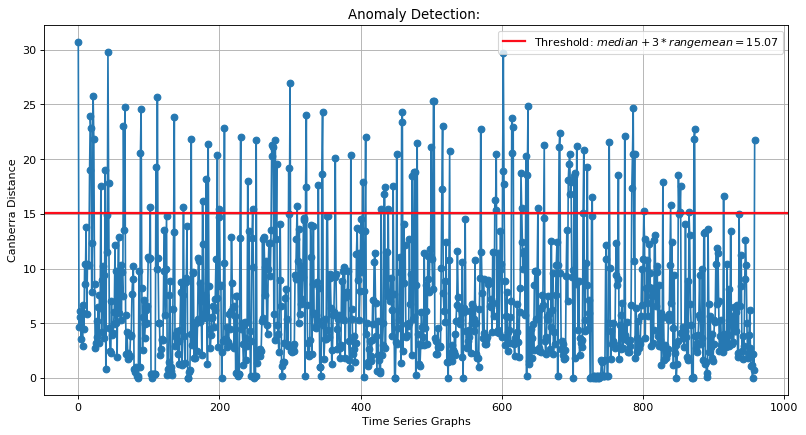
\includegraphics[height=0.6\linewidth,width=\linewidth]{fig/netsimile/anomalie_4}
	\caption{Ausrei�er Score DARPA}
	\label{img:netsimile:anomalie_4}
\end{figure}

\subsection{Anwendung des Algorithmus auf Zeitreihen}
\label{sec:ns-ts-1}

Wird der Algorithmus auf Zeitreihen anwendet, entsteht folgendes Problem. Bei der Transformation der Daten entstehen vollst�ndige Graphen, wodurch die strukturellen Eigenschaften identisch werden, sowie die daraus resultierenden Merkmale, wie in der Abbildung verdeutlicht werden soll. 

\usetikzlibrary{graphs,graphs.standard}
\begin{figure}[H]
	\centering
	\begin{tikzpicture}
		\graph[nodes={draw, circle,fill=black!20,minimum size = 6mm}, clockwise, empty nodes, radius=4cm, n=11] { subgraph K_n };
	\end{tikzpicture}
	\caption{Vollst�ndiger Graph mit 11 Knoten}
	\label{img:netsimile:graph_11}
\end{figure}

So hat bspw. das Feature $|E^{\circ}_{ego(i)}|$ keine Aussagekraft in einem vollst�ndigen Graphen, da jeder Knoten die gleiche Anzahl Kanten in seinem Ego-Netzwerk aufweist. Subtrahiert man also vom durchschnittlichen Signaturvektor aller Graphen die einzelnen Signaturvektoren, so erh�lt man den Wert 0 f�r alle Headmaps sowie den Threshold (vgl. \autoref{img:netsimile:heatmap_1}, \autoref{img:netsimile:anomalie_1}).

Somit m�ssen hier f�r diese Art von Graphen andere Features extrahiert werden. Au�erdem ist die Laufzeit in gro�en Datens�tzen, wie bspw. dem Darpa-Datensatz mit 3h Berechnungszeit nicht gerade performant.

Aus diesem Grund werden aus dem Netsimile lediglich die Ans�tze der Feature Extrahierung �bernommen, die Aggregationen ,die Distanzbildung zweier Signaturvektoren, sowie der Threshold f�r die Ausrei�eridentifizierung.

Das hei�t die Netzwerke der Zeitreihe werden nicht in ein Graphen Objekt umgewandelt, sondern als Adjazenzmatrix gespeichert. Dadurch k�nnen die Features deutlich effizienter berechnet werden. Zudem werden lediglich Features verwendet, die f�r vollst�ndige Graphen geeignet sind. Dabei werden folgende Features neu eingef�hrt:



\workTodo{n-te Wurzel bei Formel f�r Geometrischen Mittelwert}
\begin{description}
	\item[$\sum_{i=1}^{n} x_i $]\hfill\\ Summe der Kantengewichte eines Knoten.
	\item[$\frac{1}{n}\sum_{i=1}^{n} x_i $]\hfill\\ Arithmetisches Mittel der Kantengewichte eines Knoten.
	\item[$ \sqrt{\prod\limits_{i = 1}^{n} x_i} $]\hfill\\ Geometrisches Mittel der Kantengewichte eines Knoten.
	\item[$
	x(p) =
	\begin{cases}
		\frac{1}{2}x_(np) +       & \quad \text{if } n \text{ is even}\\
		-(n+1)/2  & \quad \text{if } n \text{ is odd}
	\end{cases}
	$]\hfill\\ Geometrisches Mittel der Kanten mit den 10\% h�chsten Kantengewichten. 
	\item[$\frac{1}{n}\sum_{i=1}^{n} x_i$]\hfill\\ Geometrisches Mittel der Kanten mit den 20\% h�chsten Kantengewichten. 
\end{description}

Von diesen Features wurde dann auch den Median, den Mittelwert, die Standardabweichung, die Schiefe, sowie die Kurtosis berechnet. Dadurch konnten erste Ausrei�er in der Zeitreihe gefunden werden (vgl. \autoref{img:netsimile:anomalie_2}).

\begin{figure}[H]
	\centering
	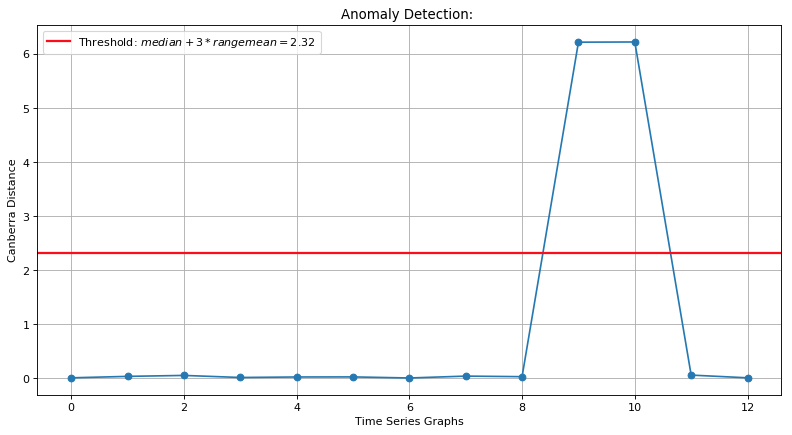
\includegraphics[height=0.6\linewidth,width=\linewidth]{fig/netsimile/anomalie_2}
	\caption{Ausrei�er Score der vollst�ndigen Graphen mit gewichteten Kanten}
	\label{img:netsimile:anomalie_2}
\end{figure}

\workTodo{Bin mir nicht sicher zu welchen Elementen die Canbarra Distanz berechnet wird.}. Des Weiteren wurde ein neuer Parameter eingef�hrt. �ber diesen kann gesteuert werden zu wie vielen vorg�nger Abschnitten die Distanz berechnet werden soll. Dadurch kann gesteuert werden wie schnell ein Algorithmus vergisst. Eine Auflistung der Parameter des Algorithmus ist in \autoref{table:parmeterNeti} zu sehen.


Um zu untersuchen, wie gut der Algorithmus funktioniert, wurde er auf Zeitreihen getestet. Als Testdaten   wurden, ein und zweidimensionale Zeitreihen der Numenta Gruppe verwendet. Diese Zeitreihen enthalten verschiedene Ausrei�er Typen, auf deren Erkennung der Algorithmus getestet wurde. Die Qualit�t der Ausrei�ererkennung wurde  mithilfe eines Punktesystem bewertet. Dabei bedeuteten 0 Punkte, Ausrei�er nicht erkannt und 4 Punkte bedeuteten Ausrei�er sehr gut erkannt. Die Parameter, welche f�r die Tests gew�hlt werden mussten, werden in \autoref{table:parmeterNeti} beschrieben.\\

\begin{table}[H]
	\centering
	\begin{tabular}{p{0.42\linewidth}|p{0.37\linewidth}|P{0.05\linewidth}|P{0.05\linewidth}}
		\toprule
		\textbf{Ausrei�er Typ}& \textbf{Datei Name}&
		\textbf{1D}&\textbf{2D}\\
		\midrule
		Einzelne Peaks & anomaly-art-daily-peaks & **& -\\
		\midrule
		Zunahme an Rauschen & anomaly-art-daily-increase-noise &****& ***\\
		\midrule
		Signal Drift & anomaly-art-daily-drift &**& -\\
		\midrule
		Kontinuierliche Zunahme der Amplitude& art-daily-amp-rise & ****& ***\\
		\midrule
		Zyklus mit h�herer Amplitude & art-daily-jumpsup &****& *\\
		\midrule
		Zyklus mit geringerer Amplitude & art-daily-jumpsdown & ****& -\\
		\midrule
		Zyklus-Aussetzer & art-daily-flatmiddle &****& ***\\
		\midrule
		Signal-Aussetzer & art-daily-nojump & ****& ***\\
		\midrule
		Frequenz�nderung & anomaly-art-daily-sequence-change &****& ***\\
		\bottomrule
	\end{tabular}
	\caption{Netsimile Time Series Perfomance}
	\label{table:performanceNeti}
\end{table}

\autoref{table:performanceNeti} zeigt die Ergebnisse der Tests. Es ist zu erkennen, dass die Qualit�t der Ausrei�er-Erkennung im eindimensionalen Fall sehr gut ist. Bei der Zeitreihe "Einzelne Peaks" werden lediglich stark abweichende Peaks erkannt. Weniger stark abweichende Peaks werden nicht erkannt. Des Weiteren wird beim Signal Drift lediglich der Anfang des Ausrei�ers detektiert. Aus diesem Grund wurde eine Bewertung mit zwei Sternen vergeben. Bei der Betrachtung der Graphiken in \autoref{sec:appendix_net_two} ist zu erkennen, dass das sechste oder siebte Intervall der Zeitreihe h�ufig als Ausrei�er markiert wird. Der Grund hierf�r ist, das bei einer Fenstergr��e von f�nf f�r die ersten f�nf Abschnitte kein Ausrei�er Score berechnet wird. Dadurch ist die Standardabweichung zu Beginn sehr niedrig wodurch Abschnitte schnell als Ausrei�er gekennzeichnet werden. Dieser Umstand wurde bei der Bewertung in \autoref{table:performanceNeti} nicht ber�cksichtigt. Im zweidimensionalen Fall ist die Qualit�t der Ausrei�er-Erkennung etwas durchwachsener. Auffallend ist, dass Zyklen mit h�herer und niedriger Amplitude nicht als Ausrei�er erkannt werden. Insbesondere ist dies auff�llig, da diese Ausrei�er Typen �blicherweise zuverl�ssig erkannt werden (vgl. \autoref{sec:rw-gl}).  Au�erdem ist der Algorithmus im zweidimensionalen Fall nicht mehr dazu in der Lage Signal Drifts zu erkennen. Andere Ausrei�er Typen k�nnen durch den Algorithmus weiterhin erkannt werden, jedoch oftmals nicht mit der selben Qualit�t. Die vollst�ndigen Ergebnisse zu den Test k�nnen in \autoref{sec:appendix_net_original} und \autoref{sec:appendix_net_two} eingesehen werden. 

\begin{table}[H]
	\centering
	\begin{tabular}{p{0.13\linewidth}|p{0.815\linewidth}}
		\toprule
		\textbf{Parameter}& \textbf{Beschreibung}\\
		\midrule
		Periodizit�t & Wie in \autoref{sec:trsnsNeti} \workTodo{Referenz sollte glaube ich autoref -> sec:trsnsNeti sein} erl�utert muss die Zeitreihe in kleinere Intervalle aufgegliedert werden. �ber diesen Parameter wird die Gr��e der Intervalle gesteuert. F�r die Tests wurde der Parameter auf 288 gesetzt, da es sich hierbei um die Saisonalit�t der Zeitreihen handelt.\\
		\midrule
		Fenstergr��e & Wie in \autoref{sec:optiNeti} erkl�rt, bestimmt dieser Parameter die Anzahl der vorangegangenen Abschnitte zu welchen die Canberra Distanz berechnet wird. Dieser Parameter wurde f�r die Tests auf 5 gesetzt.\\
		\midrule
		Abweichung & Legt fest ab wann es sich bei einem Abschnitt um einen Ausrei�er handelt. Der Parameter wurde f�r die Tests auf 3 gesetzt. Bedeutet wenn der Ausrei�er Score um das dreifache der Standardabweichung vom Durchschnitt abweicht, wird der Abschnitt als Ausrei�er gekennzeichnet.\\
		\bottomrule
	\end{tabular}
	\caption{Parameter Netsimile Zeitreihen}
	\label{table:parmeterNeti}
\end{table}


\workTodo{Die beiden Tabellen zusammenf�hren}
%\begin{table}[H]
%	\centering
%	\begin{tabular}{p{0.18\linewidth}|p{0.19\linewidth}|P{0.05\linewidth}|p{0.35\linewidth}|p{0.09\linewidth}}
%		\bottomrule
%		\textbf{Ausrei�er Typ}& \textbf{Datei Name}&
%		\textbf{1D}&\textbf{Beschreibung}&\textbf{Laufzeit}\\
%		\midrule
%		Einzelne Peaks & anomaly-art-daily-peaks & **& Zwei gemeinsame Peaks werden erkannt, Einzelne eher schlecht
%		&61min\\
%		\midrule
%		Zunahme an Rauschen & anomaly-art-daily-increase-noise &****& Ausrei�er wird erkannt&51\\
%		\midrule
%		Signal Drift & anomaly-art-daily-drift &**& Nur zwei von vier Ausrei�er werden erkannt
%		Die letzten zwei werden also normal definiert
%		&57min\\
%		\midrule
%		Kontinuierliche Zunahme der Amplitude& art-daily-amp-rise & ****& Ausrei�er werden erkannt
%		&54min\\
%		\midrule
%		Zyklus mit h�herer Amplitude & art-daily-jumpsup &****& Ausrei�er werden erkannt
%		&50\\
%		\midrule
%		Zyklus mit geringerer Amplitude & art-daily-jumpsdown & ****& Ausrei�er werden erkannt
%		&51min\\
%		\midrule
%		Zyklus-Aussetzer & art-daily-flatmiddle &****& Ausrei�er werden erkannt
%		&62min\\
%		\midrule
%		Signal-Aussetzer & art-daily-nojump & ****& Ausrei�er werden erkannt
%		&65min\\
%		\midrule
%		Frequenz�nderung & anomaly-art-daily-sequence-change &****& Ausrei�er werden erkannt
%		&49min\\
%		\bottomrule
%	\end{tabular}
%	\caption{Urspr�nglicher Netsimile Performance}
%	\label{table:performanceNeti}
%\end{table}

\workTodo{Die Bilder noch einordnen bspw. im Anhang. Im Text darauf verweisen. }

Dadurch ist die Ausrei�ererkennung von Zeitreihen in Graphen nicht m�glich. F�gt man die Gewichtung als weiteres Feature hinzu, wird hier eine erste Betrachtung der Ausrei�er m�glich. Der Graph 10 wird hier wie erhofft als Ausrei�er identifiziert.


\workTodo{bis hierhin gilt der letzte Kommentar}


\newpage
\section{MIDAS}
\label{sec:midas}
\workTodo{In diesem Kapitel werden grundlegende Themen behandelt, die im Rahmen des Forschungsprojekts zum Verst�ndnis der Ausrei�er-Erkennung in Graphen gedient haben.}


Erst erkl�ren wie der MIDAS funktioniert. Und zum Laufen gebracht mit Graphen �ber die Zeit ENRON \& DARPA. Im Anschluss auf Zeitreihendaten angewendet.


\subsection{Grundlagen}
\label{sec:mc-gl}
\workTodo{Einf�hrung in den Algorithmus, NodeHash- sowie EdgeHash-Funktionen beschreiben}

MIDAS, Eng. \textit{Microcluster-Based Detector of Anomalies in Edge Streams}, steht f�r einen Algorithmus, der pl�tzlich auftretende Ausbr�che von Aktivit�ten in einem Netzwerk bzw. Graphen erkennt. Dieses vermehrte Auftreten von Aktivit�ten zeigt sich durch viele sich wiederholende Knoten- und Kantenpaare in einem sich zeitlich entwickelnden Graphen, die Mikrocluster bezeichnet werden. Mikrocluster bestehen demnach aus einem vermehrten Vorkommen eines einzigen Quell- und Zielpaares bzw. einer Kante $(u,v)$  \workTodo{Folgender Absatz kann vor der Beschreibung des Algorithmus eingef�gt werden, wie im Paper auch} Dies geschieht in Echtzeit, wobei jede Kante in konstanter Zeit und Speicher verarbeitet wird. In der Theorie garantiert er eine False-positive-Wahrscheinlichkeit und ist durch einen 162 bis 644 mal schnelleren Ansatz, sowie einer 42\% bis 48\% h�here Genauigkeit, im Hinblick auf die AUC, sehr effektiv. \citep[vgl.][S.~1]{MIDAS}

Anwendungsf�lle f�r MIDAS sind die Erkennung von Anomalien in Computer-Netzwerken, wie SPAM oder DoS-Angriffe oder Anomalien in Kreditkartentransaktionen.


\subsubsection{Count-Min-Sketch}
\label{sec:mc-gl-cms}
Damit die relevanten Informationen f�r den Algorithmus mit einem konstanten Speicher verarbeitet werden, wird Count-Min-Sketch genutzt, dass eine Streaming-Datenstruktur mithilfe der Nutzung von Hash-Funktionen entspricht. Count-Min-Sketch z�hlt somit die Frequenz einer Aktivit�t bei Streaming-Daten. Diese Datenstruktur hat ebenfalls den Vorteil, dass man zu Beginn keine Kenntnis �ber die Anzahl an Quell- und Zielpaaren haben muss. \citep{CMS04}

MIDAS verwendet zwei Arten von CMS. Die erste Variante $s_{uv}$ wird als die Anzahl an Kanten von $u$ zu $v$ bis zum aktuellen Zeitpunkt $t$ definiert. Durch die CMS-Datenstruktur werden alle Z�hlungen von $s_{uv}$ approximiert, sodass jederzeit eine ann�hernde Abfrage $\hat{s}_{uv}$ erhalten werden kann.
Die zweite Variante $a_{uv}$ wird als die Anzahl an Kanten  von $u$ zu $v$ im aktuellen Zeitpunkt $t$ definiert. Dieser CMS ist identisch zu $s_{uv}$, wobei bei jedem �bergang zum n�chsten Zeitpunkt die Datenstruktur zur�ckgesetzt wird. Dadurch resultiert aus dem CMS f�r den aktuellen Zeitpunkt die ann�hernde Abfrage $\hat{a}_{uv}$. \citep[vgl.][S.~3]{MIDAS}


\subsubsection{Erkennung von Mikrocluster}
\label{sec:mc-gl-dm}

Mithilfe der N�herungswerte $\hat{s}_{uv}$ und $\hat{a}_{uv}$ ist das Detektieren von Mikroclustern m�glich. Hierzu wird der mittlere Pegel \workTodo{andere �bersetzung f�r mean level?} (\dah die durchschnittliche Rate mit der Kanten erscheinen) betrachtet. Es wird hierbei angenommen, dass dieser f�r den aktuellen Zeitpunkt (\zB $t = 10$) �quivalent ist zu dem vor dem aktuellen Zeitpunkt ($t < 10$). Dadurch wird die Annahmen vermieden, dass die Daten auf einer bestimmten zugrundeliegenden Verteilung basieren oder Stationarit�t �ber die Zeit aufweisen.
\\
\\
Durch die genannte Annahme lassen sich vergangene Kanten in zwei Klassen einteilen. Eine f�r den aktuellen Zeitpunkt $t = 10$ und eine f�r alle vergangenen Zeitpunkte $t < 10$. Hierbei betr�gt die Anzahl der Ereignisse zum Zeitpunkt $t = 10$ $a_{uv}$ und die Anzahl der Kanten in vergangenen Zeitpunkten $t < 10$ ist $s_{uv} - a_{uv}$.
\\
\\
Die Auswertung der Daten kann mithilfe des chi-squared goodnes-of-fit test erfolgen. Hierbei wird die Summe der Klassen $t = 10$ und $t < 10$ f�r $\frac{(\text{beobachtet} - \text{erwartet})^2}{\text{erwartet}}$ bestimmt. Bei einer Gesamtanzahl von $s_{uv}$ Kanten ergibt sich, auf Basis eines mittleren Pegels \workTodo{wie oben andere bezeichnung?}, f�r $t = 10$ eine erwartete Anzahl von $\frac{s_{uv}}{t}$ Kanten \workTodo{oder ereignisse?}. Analog hierzu ergibt sich f�r $t < 10$ eine erwartete Anzahl an $\frac{t - 1}{t}s_{uv}$ vergangenen Kanten. Daraus ergibt sich f�r die chi-squared Statistik \cite[vgl.][S.~3]{MIDAS}:

\begin{align}
	\chi^2 &= \frac{\left(\text{beobachtet}_{(t = 10)} - \text{erwartet}_{(t = 10)}\right)^2}{\text{erwartet}_{(t = 10)}} \nonumber \\
	&+ \frac{\left(\text{beobachtet}_{(t < 10)} - \text{erwartet}_{(t < 10)}\right)^2}{\text{erwartet}_{(t < 10)}} \nonumber \\
	&= \frac{\left(a_{uv} - \frac{s_{uv}}{t}\right)^2}{\frac{s_{uv}}{t}} + \frac{\left(\left(s_{uv} - a_{uv}\right) - \frac{t - 1}{t}s_{uv}\right)^2}{\frac{t - 1}{t}s_{uv}} \nonumber \\
	&= \frac{\left(a_{uv} - \frac{s_{uv}}{t}\right)^2}{\frac{s_{uv}}{t}} + \frac{\left(a_{uv} - \frac{s_{uv}}{t}\right)^2}{\frac{t - 1}{t}s_{uv}} \nonumber \\
	&= \left(a_{uv} - \frac{s_{uv}}{t}\right)^2\frac{t^2}{s_{uv}(t - 1)}
	\label{eqn:midas:chi2}
\end{align}

Die Gr��en $a_{uv}$ und $s_{uv}$ k�nnen, mithilfe der CMS-Datenstruktur, approximiert werden. Daraus ergibt sich, unter Verwendung der approximierten Gr��en $\hat{a}_{uv}$ und $\hat{s}_{uv}$, der folgende Anomaly Score \cite[vgl.][S.~4]{MIDAS}:

\begin{equation}
	score((u,v,t)) = \left(\hat{a}_{uv} - \frac{\hat{s}_{uv}}{t}\right)^2\frac{t^2}{\hat{s}_{uv}(t - 1)}
	\label{eqn:midas:score}
\end{equation}

Mithilfe des in \autoref{eqn:midas:score} angegeben Anomaly Score l�sst sich eine neue Kante $(u,v)$ zum Zeitpunkt $t$ bewerten. Dieser wird in einem bin�ren Entscheidungsverfahren verwendet, um zu bestimmen, ob es sich bei einer neuen Kante um Anomalie handelt oder nicht. Die Wahrscheinlichkeit von false positive Ergebnissen soll hierbei nicht einen benutzerdefinierten Schwellenwert $\epsilon$ �bersteigen. CMS-Datenstrukturen mit einer angemessenen Gr��e besitzen die Eigenschaft, dass die Approximationen $\hat{a}_{uv}$, f�r beliebige $\epsilon$ und $\nu$, folgende Vorschrift mit einer Wahrscheinlichkeit von mindestens $1 - \frac{\epsilon}{2}$ erf�llen:

\begin{equation}
	\hat{a}_{uv} \leq a_{uv} + \nu \cdotp N_t
\end{equation}

$N_t$ beschreibt hierbei die Anzahl an Kanten zum Zeitpunkt $t$. Eine weitere Eigenschaft der CMS-Datenstrukturen ist, dass diese die tats�chlichen Anzahl an Kanten nur �berbewerten k�nnen:

\begin{equation}
	s_{uv} \leq \hat{s}_{uv}
\end{equation}

Der in \autoref{eqn:midas:score} gegebene Score kann wie folgt angepasst werden:

\begin{equation}
	\~{a}_{uv} = \hat{a}_{uv} - \nu N_t
\end{equation}

Daraus l�sst sich die in \autoref{eqn:midas:chi2} gegebene Statistik anpassen:

\begin{equation}
	\tilde{\chi}^2 = \left(\tilde{a}_{uv} - \frac{s_{uv}}{t}\right)^2\frac{t^2}{s_{uv}(t - 1)}
	\label{eqn:midas:chi2angepasst}
\end{equation}

Bei Verwendung der Teststatistik in \autoref{eqn:midas:chi2angepasst} und eines Schwellenwertes von $\chi^2_{1 - \frac{\epsilon}{2}}(1)$ ergibt sich eine Wahrscheinlichkeit f�r ein false positive Ergebnis von h�chstens $\epsilon$:

\begin{equation}
	P\left(\tilde{\chi}^2 > \chi^2_{1 - \frac{\epsilon}{2}}(1)\right) < \epsilon
	\label{eqn:midas:prob}
\end{equation}

Der Term $\chi^2_{1 - \frac{\epsilon}{2}}(1)$ beschreibt hierbei das $1 - \frac{\epsilon}{2}$-Quantil.

\subsubsection{MIDAS-R}
Bei dem MIDAS-R Algorithmus handelt es sich um eine Erweiterung des MIDAS Algorithmus. Das R steht hierbei f�r den Relationalen Ansatz des MIDAS-R Algorithmus. Dabei wird versucht die r�umliche oder zeitliche Verkn�pfung zwischen Kanten st�rker zu ber�cksichtigten. Es werden hierzu zwei neue Konzepte eingef�hrt \citep[vgl.][S.~4]{MIDAS}.

\textbf{Temporal Relations: }Durch diesen Ansatz soll der Algorithmus mehr zeitliche Flexibilit�t erhalten. Dabei sollen Kanten aus der j�ngsten Vergangenheit auch in einem neuen Zeitabschnitt ber�cksichtigt werden. Allerdings reduziert um eine bestimmte Gewichtung. Anstatt die CMS Datenstruktur nach jedem Zeitabschnitt zu reseten, werden die Gewichte hierbei um einen bestimmten Prozentsatz reduziert \citep[vgl.][S.~4]{MIDAS}.

\textbf{Spatial Relations: }Hierbei werden zwei neue Features eingef�hrt um verschiedene Ausrei�er-Typen identifizieren zu k�nnen. Die neuen Features werden hierbei in einer CMS Datenstrukturen gespeichert. Der Algorithmus speichert demzufolge diese drei Features:

\begin{description}
	\item[$ $]\hfill\\ Anzahl an Kanten zwischen Knoten u un Knoten v. Dieses Feature wird auch vom MIDAS Algorithmus verwendet.
	\item[$ $]\hfill\\ Gesamtanzahl an Nachbarknoten eines Knoten u.
	\item[$  $]\hfill\\ Aktuelle Anzahl an Nachbarknoten eines Knoten u.
\end{description}

Aus diesen drei Features wird anschlie�end ein Ausrei�er Score abgeleitet.
 \citep[vgl.][S.~5]{MIDAS}


\section{Ausrei�er-Erkennung in Graphen}
\label{sec:m-ex}
\workTodo{ausformulieren}

\begin{figure}[H]
	\centering
	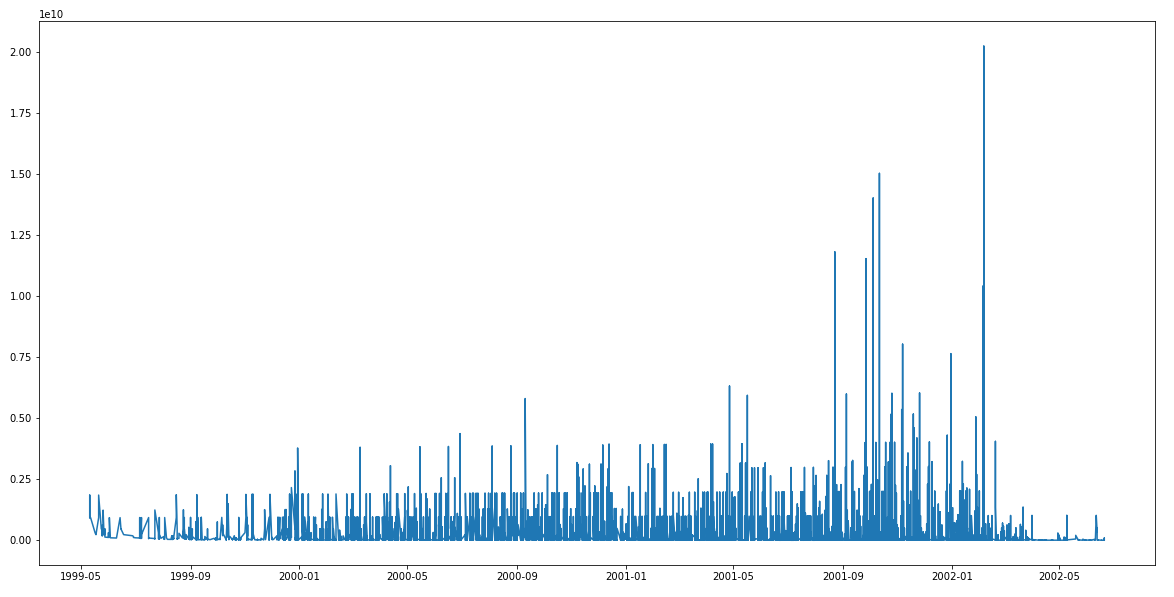
\includegraphics[height=0.6\linewidth,width=\linewidth]{fig/midas/Enron_Anomaly}
	\caption{Der Ausrei�er-Score �ber die Zeit beim ENRON-Datensatz}
	\label{img:midas:enron_anomaly}
\end{figure}



\begin{figure}[H]
	\centering
	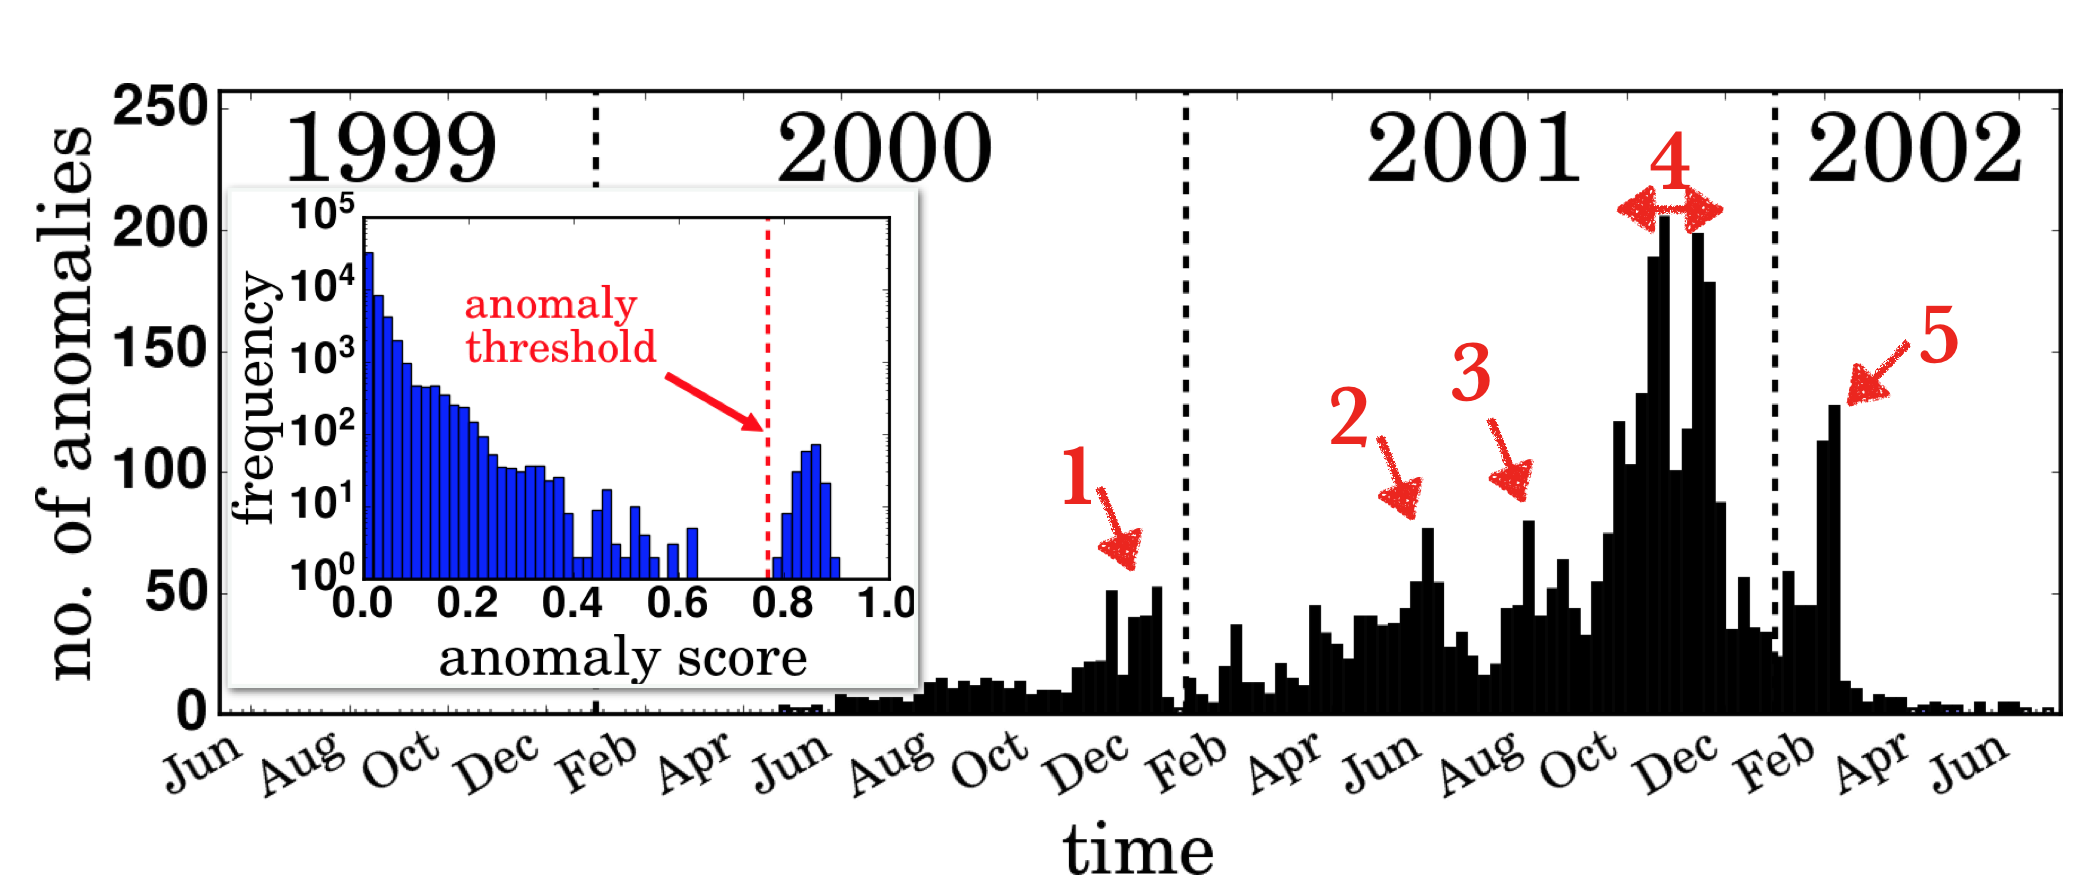
\includegraphics[height=0.4\linewidth,width=\linewidth]{fig/midas/Enron_Label}
	\caption{Die Ausrei�er des SEDANSPOT-Algorithmus}
	\label{img:midas:enron_label}
\end{figure}

Die Herausforderung geeignete \textit{labels} f�r die Datens�tze zu finden wird in zwei Schritten einged�mmt. 

Zum einen werden Erkenntnisse aus dem Schaubild des SEDANSPOT-Algorithmus gewonnen \workTodo{Quelle eingeben}. Hierbei kann man sehen, dass beide Algorithmen einen �hnlichen Verlauf vorweisen. 
Im n�chsten Schritt wird die selbe Vorgehensweise wie aus dem SEDANSPOT-Paper gew�hlt und die ENRON Timeline \workTodo{Quelle einf�gen wie bei Datensatz-Kapitel} zur Erhebung von m�glichen Auswirkungen f�r die Ausrei�er hinzugezogen.

Die \autoref{tab:enrontime} bietet eine �bersicht der historischen Ereignisse, die die Ausrei�er des MIDAS-Algorithmus erkl�ren. Im Vergleich zum SEDANSPOT-Algorithmus werden mehr Ausrei�er erkannt.
  
\begin{table}[h!]
	\centering
    \begin{tabular}{p{0.05\linewidth}|p{0.89\linewidth}}
	\toprule
	1. & Aktie erreicht Allzeithoch. Federal Energy Regulatory Commission ordnet Untersuchung an.\\
	\midrule
	2. & \textbullet Viertelj�hrliche Telefonkonferenz zur Finanzsituation und erste Symptome eines Problems. \newline \textbullet \enquote{Geheimes} Treffen -- Schwarzenegger, Lay, Milken. Angebot zur Rettung der Deregulierung. \\
	\midrule
	3. & \textbullet Skilling (CEO) k�ndigt. Mitarbeiterin warnt Lay (Gr�nder) vor Pleite. Skilling verkauft seine Aktien. \newline \textbullet Enron ver�ffentlicht 618 Mio. \$ Verlust. Interessenskonflikt wird untersucht und Akten vernichtet. \\
	\midrule
	4. & \textbullet Beginn der Strafermittlung. Lay's R�cktritt \newline \textbullet Internen Ermittlung verteilt die Schuld auf F�hrungskr�fte und den Vorstand \\
	\bottomrule
\end{tabular}
	\caption{�bersicht �ber historische Ereignisse, die den Ausrei�ern zuzuordnen sind}
	\label{tab:enrontime}
\end{table}




\begin{figure}[H]
	\centering
	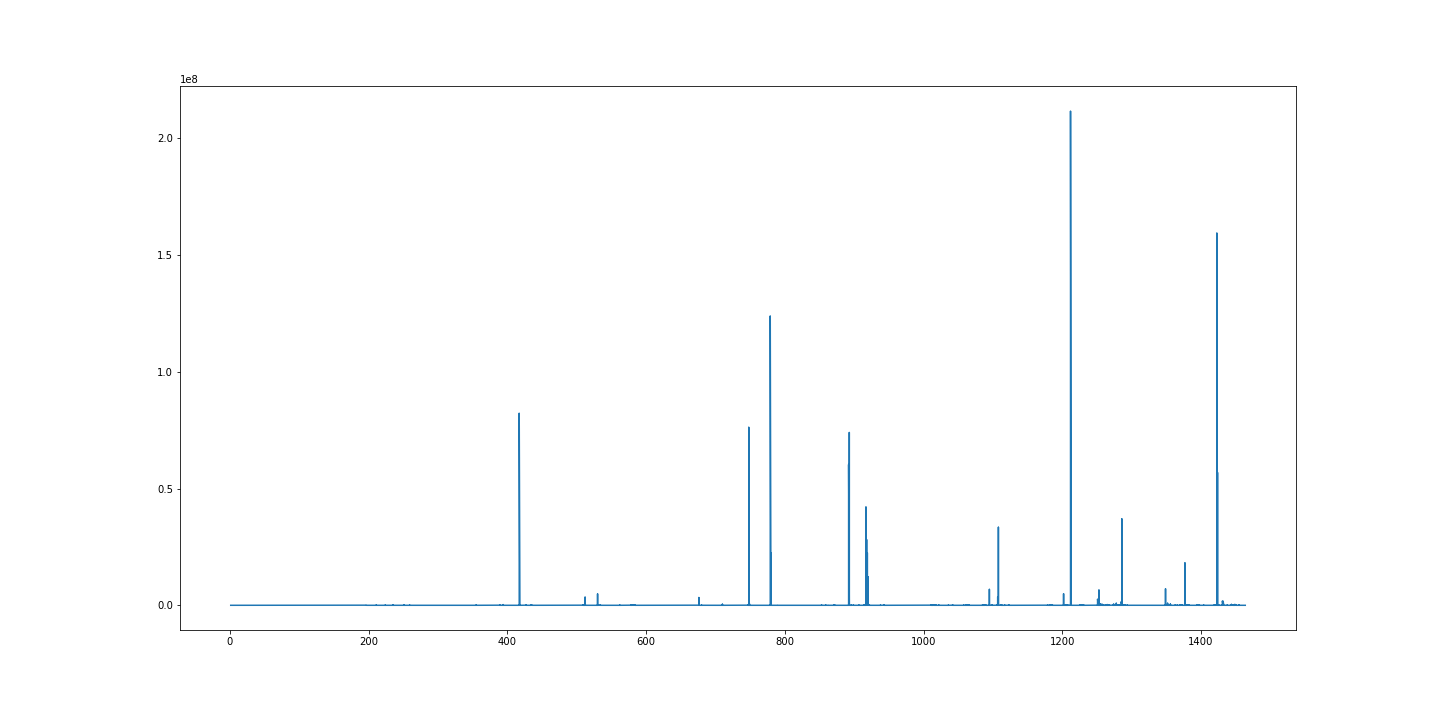
\includegraphics[height=0.6\linewidth,width=\linewidth]{fig/midas/Darpa_Anomaly}
	\caption{Der Ausrei�er-Score �ber die Zeit beim DARPA-Datensatz}
	\label{img:midas:darpa_anomaly}
\end{figure}

Bei der Anwendung des MIDAS auf dem DARPA-Datensatz sieht man sehr sch�n einzelne Ausrei�er, die entdeckt wurden. F�r diesen Datensatz gibt es, speziell f�r MIDAS entwickelt, einen \textit{ground truth}, der die \textit{labels} f�r diesen Datensatz zur Verf�gung stellt.

Bei der Berechnung der \dq Area under the Curve \dq\space f�r die ermittelten Ausrei�er-Scores wird ein Wert von $0.9172724836793507$ berechnet. Das bedeutet, dass der MIDAS-Algorithmus mit einer Wahrscheinlichkeit von ca. 91,73\% die Kanten des Datensatzes richtig klassifiziert.  

Somit kann festgehalten werden, dass MIDAS ein sehr guter Algorithmus ist bei der Erkennung von Ausrei�ern in Graphen und eine sehr hohe Genauigkeit erreicht.

\workTodo{Schwierigkeit geeignete Datens�tze zu finden, dazu gibt es ein Paper. Wenn man die Anomalyscores als gewichte nimmt, kommen Graphen in Networkx raus in denen man die anomalous nodes identifizieren kann dabei sollten es Edges sein}


\section{Ausrei�er-Erkennung in Zeitreihen}
\label{sec:resultsOTs}
\workTodo{Tabelle wie f�r Netsimile einf�gen bzgl. den verschiedenen Numenta-Datens�tzen. Bisher nicht dringlich gewesen, da MIDAS schlecht ist und wir das f�r den abstract nicht ben�tigen}

Um den MIDAS Algorithmus auf Zeitreihen anwenden zu k�nnen muss die Zeitreihe, wie in \autoref{chap:trsnsMidas} beschrieben, zun�chst in verschiedene Netzwerke umgewandelt werden. Bei den Tests konnte festgestellt werden, dass der MIDAS Algorithmus nicht dazu in der Lage ist Ausrei�er in Zeitreihen zu erkennen. Die vollst�ndigen Ergebnisse der Tests k�nnen in \autoref{chap:appendix_midas_ts} eingesehen werden. Hierbei ist jedoch der Verlauf des Ausrei�er Scores schwierig zu interpretieren. Es ist zu erkennen, das der Ausrei�er-Score zu Beginn eines jeden Abschnitts sehr hoch ist, am Ende des Abschnitts ist der Ausrei�er Score hingegen relativ niedrig. Grund hierf�r ist, das die Anzahl an Kanten zu Beginn eines Abschnittes im Verh�ltnis zu der Anzahl an Kanten aus den vorangegangenen Abschnitten deutlich niedriger ist. Im weiteren Verlauf werden weitere Kanten innerhalb des Abschnitts hinzugef�gt. Dadurch gleicht sich die Anzahl an Kanten innerhalb der Abschnitte an und der Ausrei�er Score sinkt.

Der MIDAS Algorithmus ist lediglich bei einer Zeitreihe dazu in der Lage den Ausrei�er zu identifizieren. Hierbei handelt es sich um die Zeitreihe mit erh�hter Amplitude (vgl. \autoref{img:midasTSresultJumpsup}). Durch den Ausschlag nach oben in der Zeitreihe entsteht ein Netzwerk, mit sehr hohen Gewichten. Die hohen Gewichte f�hren zu einer erh�hten Anzahl an Kanten, was schlussendlich zu einem Ausschlag des Ausrei�er Scores f�hrt. Die erh�hte Anzahl an Kanten f�hrt ebenfalls dazu das der Abschnitt mit dem Ausrei�er in der Abbildung deutlich breiter ist als die anderen. Bei anderen Ausrei�er Typen sind die Differenzen zwischen den verschiedenen Elementen der Zeitreihe nicht so gro�. Dadurch ergeben sich keinerlei hohe Kantengewichte und der Ausrei�er kann nicht erkannt werden.


\begin{figure}[h]
	\centering
	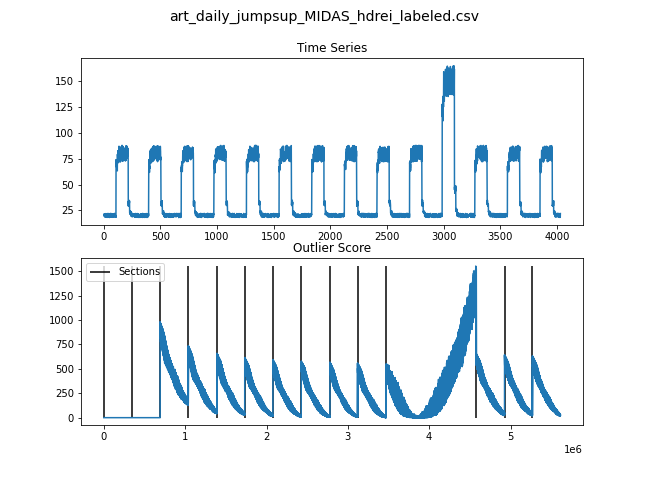
\includegraphics[width=0.5\textwidth]{fig/resultsMidasTS/art_daily_jumpsup_MIDAS_hdrei_labeled_result.png}
	\caption{MIDAS Algorithmus angewandt auf Zeitreihe mit einer erh�ten Amplitude.}
	\label{img:midasTSresultJumpsup}
\end{figure}

Teilweise f�hren die Ausrei�er auch zu besonders wenigen Kanten (vgl. \autoref{img:midasTSresultsFlatSeqChange}). Bei diesem Ausrei�er Typ sind alle Werte auf der selben Ebene. Dadurch gehen die Kantengewichte gegen Null. Dies f�hrt zu einem sehr kurzen Abschnitt in der Abbildung (Der Abschnitt wurde mit einem Pfeil markiert). \workTodo{Noch Pfeil in Graphik einf�gen} Des weiteren ergibt sich durch die Ausrei�er eine leicht ver�nderte Anzahl an Kanten in dem Abschnitt mit dem Ausrei�er (vgl. \autoref{img:midasTSresultsFlatSeqChange}). Die Abweichungen sind jedoch so gering, dass es nicht zu einem starken Anstieg des Ausrei�er Scores f�hrt.
\label{sec:resultTSwithoutMidas}

\begin{figure}[h]
	\centering
	\subfloat[Zeitreihe mit Zyklus Aussetzter]{
		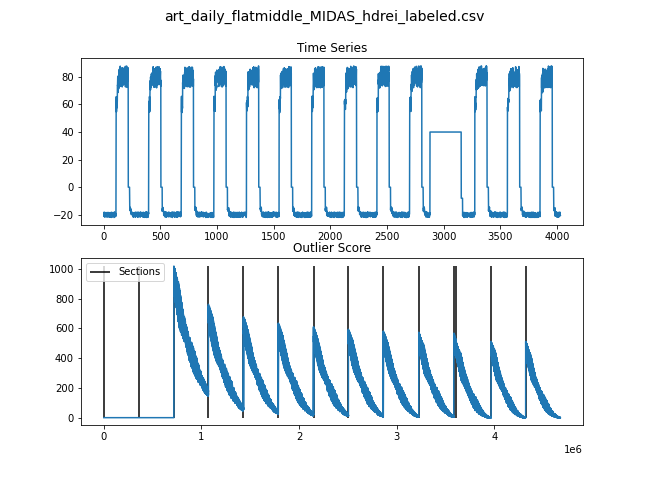
\includegraphics[width=0.5\textwidth]{fig/resultsMidasTS/art_daily_flatmiddle_MIDAS_hdrei_labeled_result.png}}
	\subfloat[Zeitreihe mit Frequenz�nderung]{
		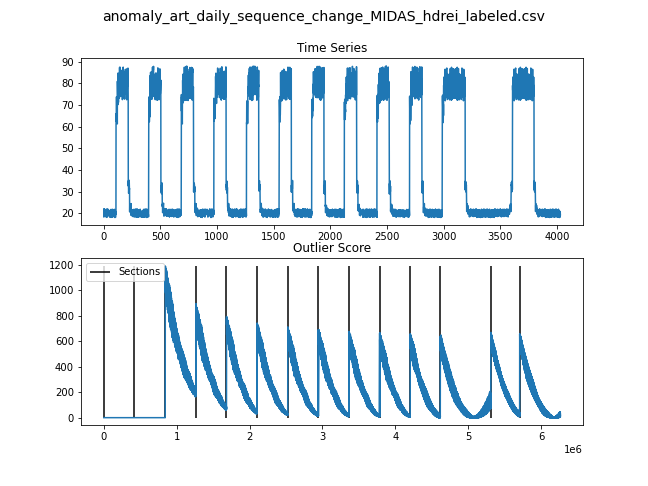
\includegraphics[width=0.5\textwidth]{fig/resultsMidasTS/anomaly_art_daily_sequence_change_MIDAS_hdrei_labeled_result.png}}
	\caption{Ausrei�er Erkennung in Zeitreihen MIDAS Algorithmus}
	\label{img:midasTSresultsFlatSeqChange}
\end{figure}

Es wurden au�erdem Tests durchgef�hrt um zu Untersuchen, wie sich der Algorithmus bei ver�nderter Fenstergr��e verh�lt (vgl. \autoref{img:midasTSresults110}). Bei den Untersuchungen in \autoref{img:midasTSresultJumpsup} und \autoref{img:midasTSresultsFlatSeqChange} wurde einer Fenstergr��e von 288 genutzt, was der Saisonalit�t der Zeitreihe entspricht. F�r dieses Experiment wurde einer Fenstergr��e von 110 verwendet. Es konnte festgestellt werden, das diese Ver�nderung keinen zus�tzlichen Nutzen erbringt. Allerdings ist der Ausschlag nach oben im Ausrei�er Score f�r die Zeitreihe mit erh�hter Amplitude noch deutlicher zu erkennen. Die anderen Ausrei�er Typen werden weiterhin nicht erkannt.

\begin{figure}[h]
	\centering
	\subfloat[Zeitreihe mit einer Frequenz�nderung]{
		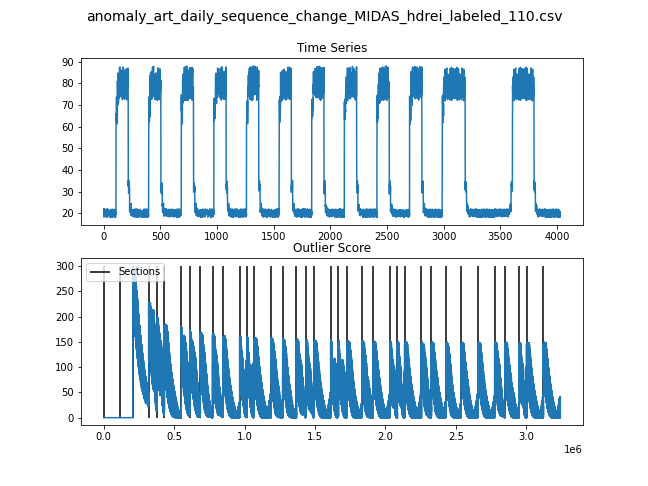
\includegraphics[width=0.5\textwidth]{fig/resultsMidasTS/anomaly_art_daily_sequence_change_MIDAS_hdrei_labeled_110_result.png}}	
	\subfloat[Zeitreihe mit erh�hter Amplitude]{
		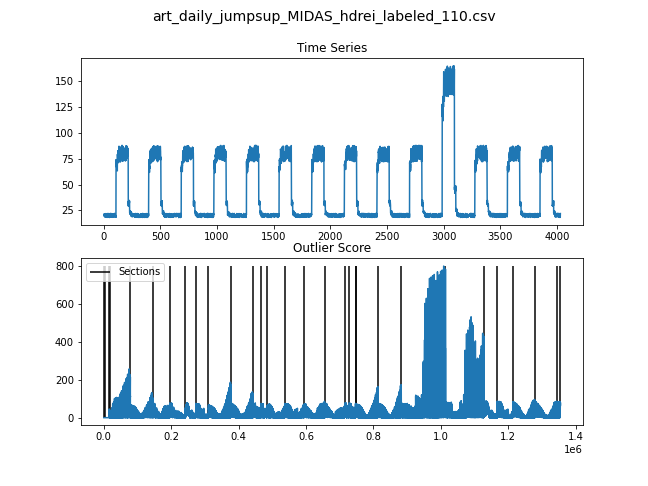
\includegraphics[width=0.5\textwidth]{fig/resultsMidasTS/art_daily_jumpsup_MIDAS_hdrei_labeled_110_result.png}}
	\caption{Ausrei�er Erkennung Zeitreihen MIDAS Algorithmus Fenstergr��e 110}
	\label{img:midasTSresults110}
\end{figure}

In einem n�chsten Schritt wurde untersucht inwiefern der MIDAS-R Algorithmus zu einer Verbesserung bei der Ausrei�er Erkennung beitragen kann (vgl. \autoref{img:midasRTSresults}). Der MIDAS-R Algorithmus ber�cksichtigt bei der Berechnung des Ausrei�er Scores f�r den aktuellen Abschnitt auch die Daten aus der j�ngsten Vergangenheit(vorangegangene Abschnitte). Aus diesem Grund erhofften wir uns durch den Einsatz des MIDAS-R Algorithmus, dass die Ausschl�ge zu beginn eines jeden Abschnitts aus bleiben, sodass Ausrei�er deutlicher hervortreten. Es konnte festgestellt werden, dass der Ausschlag des Ausrei�er Scores zu Beginn der Abschnitte deutlich kleiner ist. Jedoch steigt der Ausrei�er Score zum Ende eines jeden Abschnitts wieder an. Es konnte somit keine Signifikante Verbesserung bei der Erkennung von Ausrei�ern erreicht werden. Insbesondere da der MIDAS-R Algorithmus ebenfalls nur den Ausrei�er in der Zeitreihe mit erh�hter Amplitude anzeigt. Somit konnte festgestellt werden, dass auch die durch den MIDAS-R Algorithmus eingef�hrten Features zu keiner Verbesserung der Ergebnisse gef�hrt haben. 
\workTodo{Vielleicht k�nnte eine Verbesserung erreicht werden wenn andere Features eingef�hrt werden w�rden.}


\begin{figure}[h]
	\centering
	\subfloat[Zeitreihe mit geringerer Amplitude]{
		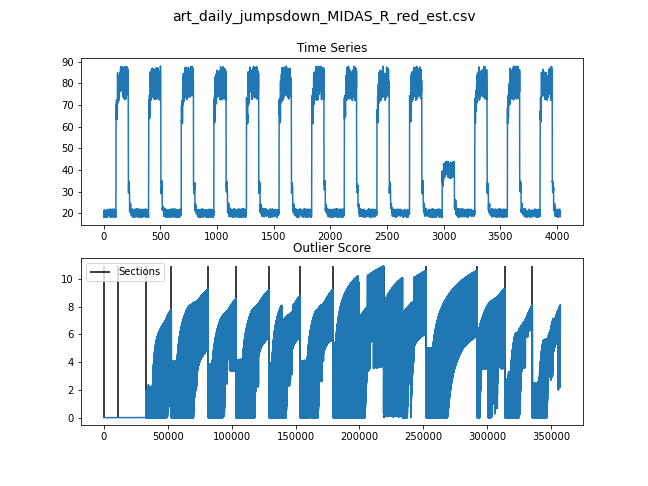
\includegraphics[width=0.5\textwidth]{fig/reultsMidasR/art_daily_jumpsdown_MIDAS_R_red_est_result}}
	\subfloat[Zeitreihe mit erh�hter Amplitude]{
		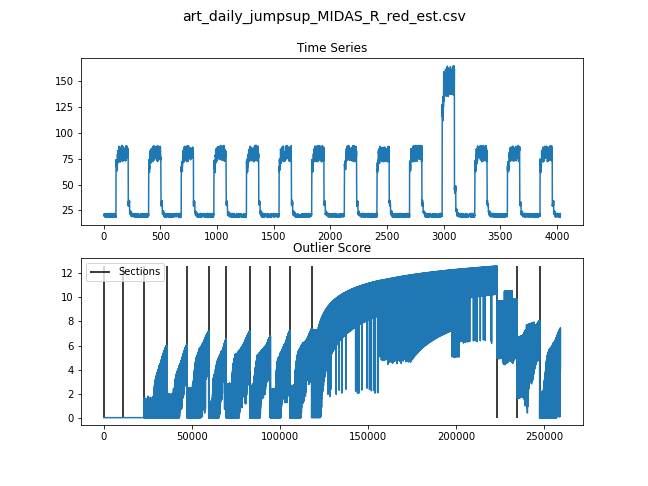
\includegraphics[width=0.5\textwidth]{fig/reultsMidasR/art_daily_jumpsup_MIDAS_R_red_est_result}}
	\caption{Ausrei�er Erkennung Zeitreihen MIDAS-R}
	\label{img:midasRTSresults}
\end{figure}




%\newpage
\section{Netsimile}
\label{sec:ns}

\subsection{Grundlagen}
\label{ssec:ns-gl}

Netsimile ist ein skalierbarer Algorithmus zur Erkennung von �hnlichkeiten, sowie Anomalien in Netzwerken unterschiedlicher Gr��en. Hierf�r wird der Datensatz in gleich gro�e Zeitintervalle unterteilt, um die daraus resultierenden Graphen auf unterschiedliche Merkmale zu untersuchen. Die Merkmale sind hierbei strukturelle Eigenschaften der einzelnen Knoten wie bspw. die Dichte eines Knotens oder die Anzahl an Nachbarn in einem Ego-Netzwerk. Die Signatur ergibt sich aus den einzelnen Aggregationen der Knoten wie bspw. der Median aus der Dichte der jeweiligen Knoten. So entsteht bspw. aus sieben Merkmalen und f�nf Aggregationen ein Signaturvektor mit 35 verschiedenen Signaturen. So erm�glicht der Signarturvektor die Beschreibung als auch den Vergleich der einzelnen Graphen. F�r den Vergleich wird die Canberra Distanz aus den beiden Signaturvektoren zweier zeitlich nebeneinander liegenden Graphen berechnet. \citep[vgl.][S.~1]{Netsimile}

Als Input f�r diesen Algorithmus wird eine Menge von $k$-anonymisierten Netzwerken mit beliebig unterschiedlichen Gr��en, die keine �berlappenden Knoten oder Kanten besitzen sollten, herangezogen werden. Das Resultat sind Werte f�r die strukturelle �hnlichkeit oder Abstands eines jeden Paares der gegebenen Netzwerke bzw. ein Merkmalsvektor f�r jedes Netzwerk. \citep[vgl.][S.~1]{Netsimile}

Netsimile durchl�uft drei Schritte, die im Folgenden erl�utert werden.

\subsubsection{Extrahierung von Merkmalen}
F�r jeden Knoten $i$ werden, basierend auf ihren Ego-Netzwerken, die folgenden Merkmale generiert:


\begin{description}
	\item[$\overline{d}_i = |N(i)|$]\hfill\\ Die Anzahl der Nachbarn (d.h. Grad) von Knoten $i$, wobei $N(i)$ die Nachbarn von Knoten $i$ beschreibt.
	\item[$\overline{c}_i$]\hfill\\ Der Clustering-Koeffizient von Knoten $i$, der als die Anzahl von Dreiecken, die mit Knoten $i$ verbunden sind, �ber die Anzahl von verbundenen Dreiecken, die auf Knoten $i$ zentriert sind, definiert ist.
	\item[$d_{N(i)}$]\hfill\\ Die durchschnittliche Anzahl der Nachbarn von Knoten $i$, die zwei Schritte entfernt sind. Dieser wird berechnet als \workTodo{Paper Seite 2 unten Formel einf�gen}
	\item[$c_{N(i)}$]\hfill\\ Der durchschnittliche Clustering-Koeffizient von $N(i)$, der als \workTodo{Paper Seite 2 unten Formel einf�gen} berechnet wird.
	\item[$|E_{ego(i)}|$]\hfill\\ Die Anzahl der Kanten im Ego-Netzwerk vom Knoten $i$, wobei $ego(i)$ das Ego-Netzwerk von $i$ zur�ckgibt.
	\item[$|E^{\circ}_{ego(i)}|$]\hfill\\ Die Anzahl der von $ego(i)$ ausgehenden Kanten. 
	\item[$|N(ego(i))|$]\hfill\\ Die Anzahl von Nachbarn von $ego(i)$. 
\end{description}

\subsubsection{Aggregierung von Merkmalen}
Im n�chsten Schritt wird f�r jeden Graphen \textit{$G_j$} eine $Knoten \times Merkmal$-Matrix $F_{G_j}$ zusammengefasst. Dieser besteht aus den Merkmalsvektoren aus Schritt 1.
Da der Vergleich von $k$-ten $F_{G_j}$ sehr aufw�ndig ist, wird f�r jede $F_{G_j}$ ein Signaturvektor $\vec{s}_{G_j}$ ausgegeben. Dieser aggregiert den Median, den Mittelwert, die Standardabweichung, die Schiefe, sowie die Kurtosis der Merkmale aus der Matrix.  

\subsubsection{Vergleich der Signaturvektoren}
\label{sec:ns-gl-cd}

F�r die Ausrei�ererkennung werden die letzten drei Graphen anhand der Canberra-Distanz-Funktion, die als �hnlichkeitsma� dient, herangezogen. Steigt die Canberra Distanz zwischen zwei Graphen oberhalb des Thresholds so wird dies im Algorithmus festgehalten. Falls der darauf folgende Graph ebenfalls oberhalb des Thresholds liegt, so wird dieser als Ausrei�er definiert. Dadurch wird die Anzahl der Ausrei�er reduziert, damit nur diejenigen identifiziert werden, bei denen ein Trend hin zu einem abnormalen Verhalten erkennbar ist.

Der Algorithmus arbeitet dabei dynamisch, da die Signaturen der Graphen in einzelne Teil-Berechnungen aufgesplittet und zwischengespeichert werden k�nnen, ohne das eine Neuberechnung notwendig ist. Der Threshold wird aus dem Median und dem Mean berechnet, welche ebenfalls Zwischengespeichert werden k�nnen und nach Bedarf um weitere Graphen erg�nzt werden k�nnen.

\FloatBarrier

\subsection{Anwendung des Algorithmus auf Netzwerkdaten}
\label{sec:ns-ext}
Beim ersten Versuch den Algorithmus auf Netzwerkdaten anzuwenden, wurde folgende Probleme festgestellt:

Der Algorithmus verwendet eine Bibliothek \textit{igraph}, welche Kanten zwischen zwei Knoten nur einmalig hinzuf�gen kann. Beim Eliminieren der Duplikate w�rde aber ein Drittel des Datensatzes nicht ber�cksichtigt werden, wodurch wertvolle Informationen bei der Ausrei�ererkennung verloren gehen w�rden. Aus diesem Grund wurden die Netzwerkdaten soweit angepasst, dass Mehrfachverbindungen zwischen zwei Kanten aufsummiert werden und als Gewichtung dieser Kante hinzugef�gt wird. 

\begin{lstlisting}[language=Python, caption=Gewichtung als neues Feature, label=lst:netsimile:code1]
for i in range(len(e_list)): 
	g.add_edge(e_list[i][0], e_list[i][1], weight=e_list[i][2])
\end{lstlisting}

Dadurch kann der Datensatz zum einen vollst�ndig analysiert werde und zum anderen konnte dadurch ein weiteres Feature hinzugef�gt werden, dass durch die f�nf verschiedenen Aggregationen den Signaturvektor um diese f�nf Werte erweitert.

Dadurch das der Datensatz zuerst eingelesen und in einen Graphen transformiert wird und anschlie�end aus dem Graphen die jeweiligen Features extrahiert werden, verliert der Algorithmus extrem an Performanz. Des weiteren wird im ersten Schritt der maximale Knoten-Wert als Gr��e des Graphens �bergeben. Wird bspw. f�r jeden Mitarbeiter eine eigene ID �bergeben und die inkrementell erh�ht, so kann es sein, dass aus einem Netzwerk mit 20 verschiedenen Knoten ein Graph erzeugt wird, der 1000 Knoten erzeugt, weil eine ID mit dem Wert 1000 vorhanden ist. Dadurch b��t die Performanz an Geschwindigkeit ein, da Iterationen nicht �ber die 20 Knoten durchgef�hrt werden, sondern �ber 1000. Hier muss entweder der Datensatz vorab angepasst werden, indem die IDs neu vergeben werden oder der Algorithmus muss grundlegend neu aufgebaut werden.

Da der Fokus auf der Anwendung von Zeitreihen liegt, wird die Optimierung erst in diesem Abschnitt erl�utert.



Das Problem hierbei ist, dass jeder Knoten eines Graphens die gleichen Features beinhalten w�rde. Dadurch w�rden die Aggregationen �berfl�ssig werden und der Signaturvektor auf sieben Features schrumpfen. Die Bildung von Cluster-Features w�re demnach nur noch bedingt m�glich und die Betrachtung an Nachbarn, unabh�ngig ob im Ego-Netzwerk oder im gesamten Netzwerk w�rde sich die Gesamtanzahl an Knoten ann�hern. Im Folgenden wird das Verh�ltnis der Features zum Durchschnitt dargestellt.

\subsubsection{Anwendung auf ENRON-Datensatz}
\label{sec:ns-enron}

Da der Enron Datensatz ebenfalls von einem anderen Paper analysiert und ver�ffentlicht wurde, k�nnen die dort erkannten Ausrei�er zum Vergleich in Form eines gelabelten Datensatz verwendet werden.
Betrachtet man in diesem Kontext den Aurei�erscore, ist gut zu erkennen, dass der Ausrei�er Ende 2001 als alleiniger herausstechender Ausrei�er auch im Ergebnis wiederzufinden ist. Grundlegend ist aber auch zu erkennen, dass die Ausrei�er sich nur sehr wenig voneinander unterscheiden, wodurch eine Klassifizierung innerhalb des Ausrei�erscores sich als schwierig erweist. Die Extrahierung weiterer Features k�nnte hier eventuell aushelfen, wobei dies nicht im Rahmen dieses Forschungsprojektes behandelt werden soll, da der Fokus auf Zeitreihen liegt. Zwecks Performanz konnte der Datensatz innerhalb von zwei Minuten analysiert werden.

\begin{figure}[H]
	\centering
	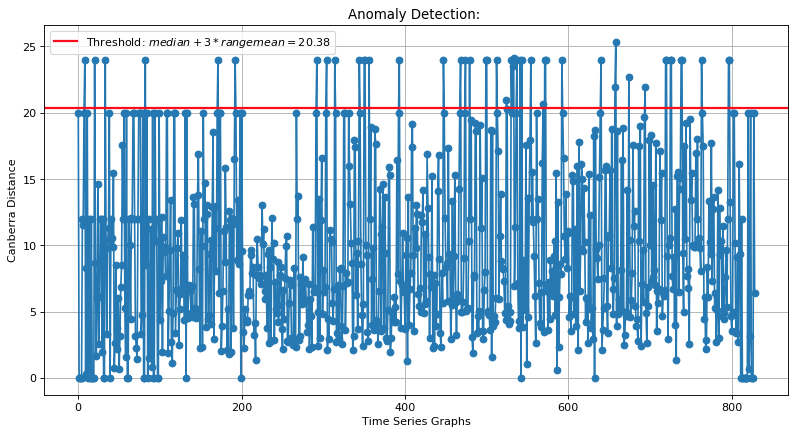
\includegraphics[height=0.6\linewidth,width=\linewidth]{fig/netsimile/anomalie_3}
	\caption{Ausrei�er Score Enron Datensatz}
	\label{img:netsimile:anomalie_3}
\end{figure}

\begin{figure}[H]
	\centering
	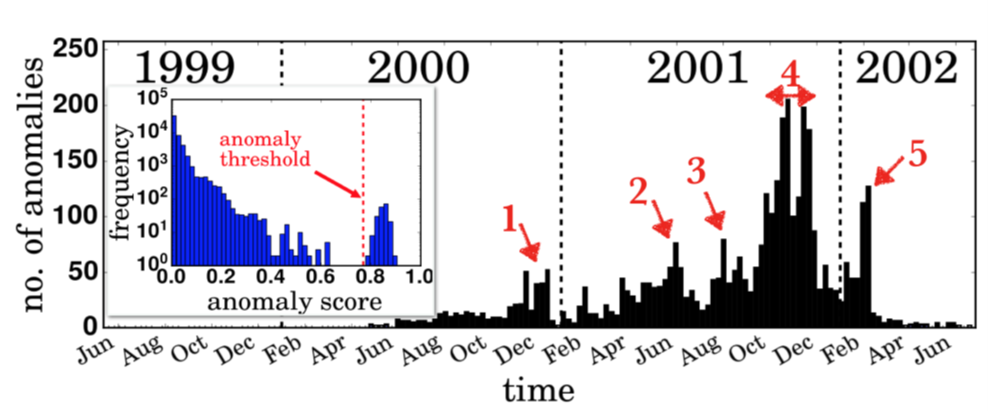
\includegraphics[height=0.6\linewidth,width=\linewidth]{fig/sedanspot}
	\caption{\workTodo{Sedanspot Caption}}
	\label{img:sedanspot}
\end{figure}

Betrachtet man die Differenz aus dem Durchschnitt der Signaturvektoren und den der Ausrei�ergraphen in einer Headmap kann man erkennen, dass die Ausrei�er vorwiegend durch besonders gro�e Ego-Netzwerke und einer hohen Anzahl an E-Mails verschuldet ist.



\begin{figure}[H]
	\centering
	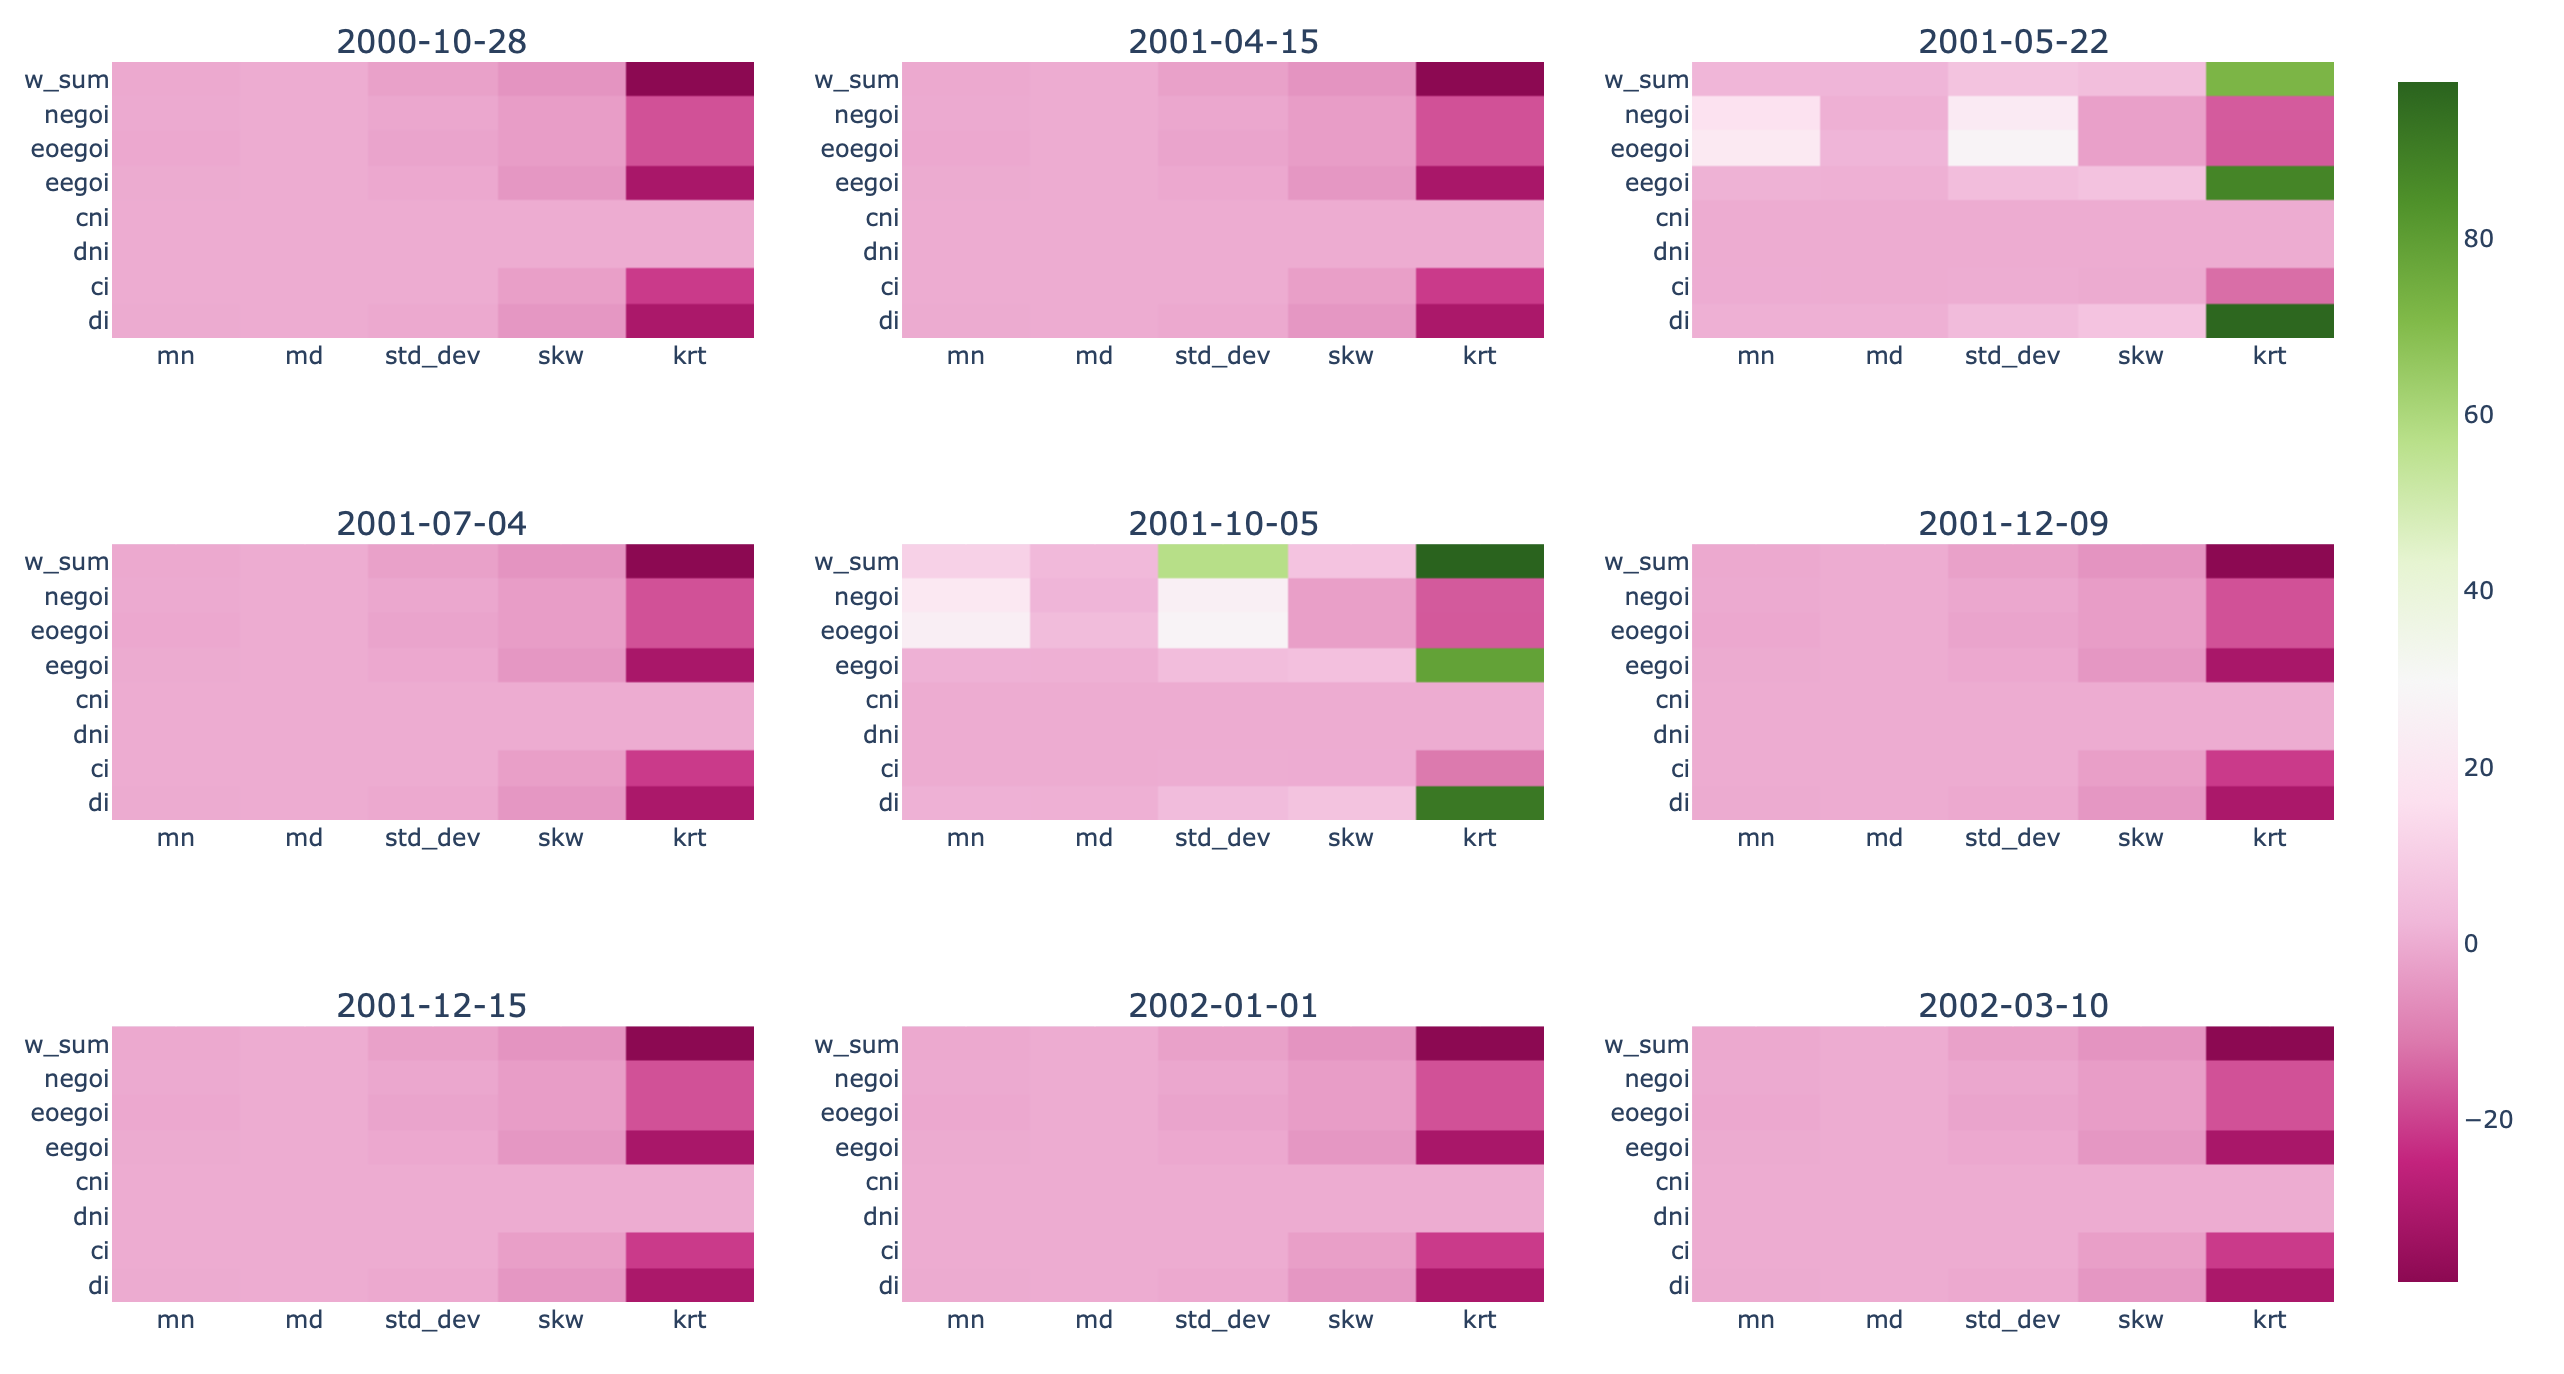
\includegraphics[height=0.8\linewidth,width=\linewidth]{fig/netsimile/heatmap_3}
	\caption{Darstellung der Ausrei�er in Heatmaps}
	\label{img:netsimile:heatmap_3}
\end{figure}

\subsubsection{Anwendung auf DARPA-Datensatz}
\label{sec:ns-darpa}

Beim Darpa Datensatz k�nnen die Aurei�er besser klassifiziert werden. Die Gr�nde k�nnen hierbei auf die Gr��e und Vielfalt des Datensatzes zur�ckgef�hrt werden. Der Enron Datensatz hat eine Gr��e von 1MB und rund 50.000 Kanten. Der Darpa Datensatz hingegen hat eine Gr��e von 50 MB mit 4.5 Mio Kanten. Die Berechnung hat dabei eine L�nge von 3h. Haben wir bei der Dateigr��e den Faktor 50 und bei der Kantenanzahl den Faktor 90, so ist bei der Berechnungszeit der Faktor 90 wiederzufinden. Betrachtet man die Laufzeit, so kann eine lineare Abh�ngigkeit zwischen Kantenanzahl und der ben�tigten Berechnungszeit festgestellt werden.

\begin{figure}[H]
	\centering
	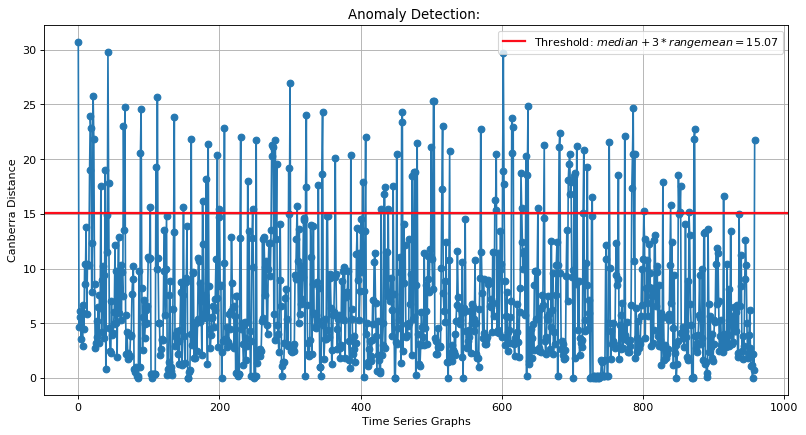
\includegraphics[height=0.6\linewidth,width=\linewidth]{fig/netsimile/anomalie_4}
	\caption{Ausrei�er Score DARPA}
	\label{img:netsimile:anomalie_4}
\end{figure}

\subsection{Anwendung des Algorithmus auf Zeitreihen}
\label{sec:ns-ts-1}

Wird der Algorithmus auf Zeitreihen anwendet, entsteht folgendes Problem. Bei der Transformation der Daten entstehen vollst�ndige Graphen, wodurch die strukturellen Eigenschaften identisch werden, sowie die daraus resultierenden Merkmale, wie in der Abbildung verdeutlicht werden soll. 

\usetikzlibrary{graphs,graphs.standard}
\begin{figure}[H]
	\centering
	\begin{tikzpicture}
		\graph[nodes={draw, circle,fill=black!20,minimum size = 6mm}, clockwise, empty nodes, radius=4cm, n=11] { subgraph K_n };
	\end{tikzpicture}
	\caption{Vollst�ndiger Graph mit 11 Knoten}
	\label{img:netsimile:graph_11}
\end{figure}

So hat bspw. das Feature $|E^{\circ}_{ego(i)}|$ keine Aussagekraft in einem vollst�ndigen Graphen, da jeder Knoten die gleiche Anzahl Kanten in seinem Ego-Netzwerk aufweist. Subtrahiert man also vom durchschnittlichen Signaturvektor aller Graphen die einzelnen Signaturvektoren, so erh�lt man den Wert 0 f�r alle Headmaps sowie den Threshold (vgl. \autoref{img:netsimile:heatmap_1}, \autoref{img:netsimile:anomalie_1}).

Somit m�ssen hier f�r diese Art von Graphen andere Features extrahiert werden. Au�erdem ist die Laufzeit in gro�en Datens�tzen, wie bspw. dem Darpa-Datensatz mit 3h Berechnungszeit nicht gerade performant.

Aus diesem Grund werden aus dem Netsimile lediglich die Ans�tze der Feature Extrahierung �bernommen, die Aggregationen ,die Distanzbildung zweier Signaturvektoren, sowie der Threshold f�r die Ausrei�eridentifizierung.

Das hei�t die Netzwerke der Zeitreihe werden nicht in ein Graphen Objekt umgewandelt, sondern als Adjazenzmatrix gespeichert. Dadurch k�nnen die Features deutlich effizienter berechnet werden. Zudem werden lediglich Features verwendet, die f�r vollst�ndige Graphen geeignet sind. Dabei werden folgende Features neu eingef�hrt:



\workTodo{n-te Wurzel bei Formel f�r Geometrischen Mittelwert}
\begin{description}
	\item[$\sum_{i=1}^{n} x_i $]\hfill\\ Summe der Kantengewichte eines Knoten.
	\item[$\frac{1}{n}\sum_{i=1}^{n} x_i $]\hfill\\ Arithmetisches Mittel der Kantengewichte eines Knoten.
	\item[$ \sqrt{\prod\limits_{i = 1}^{n} x_i} $]\hfill\\ Geometrisches Mittel der Kantengewichte eines Knoten.
	\item[$
	x(p) =
	\begin{cases}
		\frac{1}{2}x_(np) +       & \quad \text{if } n \text{ is even}\\
		-(n+1)/2  & \quad \text{if } n \text{ is odd}
	\end{cases}
	$]\hfill\\ Geometrisches Mittel der Kanten mit den 10\% h�chsten Kantengewichten. 
	\item[$\frac{1}{n}\sum_{i=1}^{n} x_i$]\hfill\\ Geometrisches Mittel der Kanten mit den 20\% h�chsten Kantengewichten. 
\end{description}

Von diesen Features wurde dann auch den Median, den Mittelwert, die Standardabweichung, die Schiefe, sowie die Kurtosis berechnet. Dadurch konnten erste Ausrei�er in der Zeitreihe gefunden werden (vgl. \autoref{img:netsimile:anomalie_2}).

\begin{figure}[H]
	\centering
	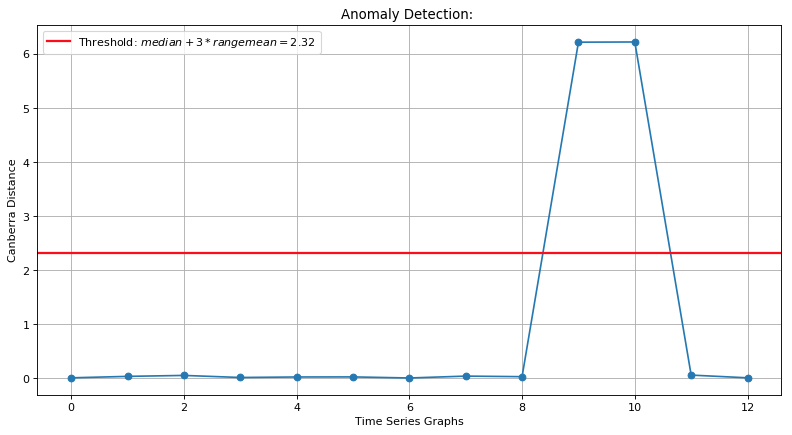
\includegraphics[height=0.6\linewidth,width=\linewidth]{fig/netsimile/anomalie_2}
	\caption{Ausrei�er Score der vollst�ndigen Graphen mit gewichteten Kanten}
	\label{img:netsimile:anomalie_2}
\end{figure}

\workTodo{Bin mir nicht sicher zu welchen Elementen die Canbarra Distanz berechnet wird.}. Des Weiteren wurde ein neuer Parameter eingef�hrt. �ber diesen kann gesteuert werden zu wie vielen vorg�nger Abschnitten die Distanz berechnet werden soll. Dadurch kann gesteuert werden wie schnell ein Algorithmus vergisst. Eine Auflistung der Parameter des Algorithmus ist in \autoref{table:parmeterNeti} zu sehen.


Um zu untersuchen, wie gut der Algorithmus funktioniert, wurde er auf Zeitreihen getestet. Als Testdaten   wurden, ein und zweidimensionale Zeitreihen der Numenta Gruppe verwendet. Diese Zeitreihen enthalten verschiedene Ausrei�er Typen, auf deren Erkennung der Algorithmus getestet wurde. Die Qualit�t der Ausrei�ererkennung wurde  mithilfe eines Punktesystem bewertet. Dabei bedeuteten 0 Punkte, Ausrei�er nicht erkannt und 4 Punkte bedeuteten Ausrei�er sehr gut erkannt. Die Parameter, welche f�r die Tests gew�hlt werden mussten, werden in \autoref{table:parmeterNeti} beschrieben.\\

\begin{table}[H]
	\centering
	\begin{tabular}{p{0.42\linewidth}|p{0.37\linewidth}|P{0.05\linewidth}|P{0.05\linewidth}}
		\toprule
		\textbf{Ausrei�er Typ}& \textbf{Datei Name}&
		\textbf{1D}&\textbf{2D}\\
		\midrule
		Einzelne Peaks & anomaly-art-daily-peaks & **& -\\
		\midrule
		Zunahme an Rauschen & anomaly-art-daily-increase-noise &****& ***\\
		\midrule
		Signal Drift & anomaly-art-daily-drift &**& -\\
		\midrule
		Kontinuierliche Zunahme der Amplitude& art-daily-amp-rise & ****& ***\\
		\midrule
		Zyklus mit h�herer Amplitude & art-daily-jumpsup &****& *\\
		\midrule
		Zyklus mit geringerer Amplitude & art-daily-jumpsdown & ****& -\\
		\midrule
		Zyklus-Aussetzer & art-daily-flatmiddle &****& ***\\
		\midrule
		Signal-Aussetzer & art-daily-nojump & ****& ***\\
		\midrule
		Frequenz�nderung & anomaly-art-daily-sequence-change &****& ***\\
		\bottomrule
	\end{tabular}
	\caption{Netsimile Time Series Perfomance}
	\label{table:performanceNeti}
\end{table}

\autoref{table:performanceNeti} zeigt die Ergebnisse der Tests. Es ist zu erkennen, dass die Qualit�t der Ausrei�er-Erkennung im eindimensionalen Fall sehr gut ist. Bei der Zeitreihe "Einzelne Peaks" werden lediglich stark abweichende Peaks erkannt. Weniger stark abweichende Peaks werden nicht erkannt. Des Weiteren wird beim Signal Drift lediglich der Anfang des Ausrei�ers detektiert. Aus diesem Grund wurde eine Bewertung mit zwei Sternen vergeben. Bei der Betrachtung der Graphiken in \autoref{sec:appendix_net_two} ist zu erkennen, dass das sechste oder siebte Intervall der Zeitreihe h�ufig als Ausrei�er markiert wird. Der Grund hierf�r ist, das bei einer Fenstergr��e von f�nf f�r die ersten f�nf Abschnitte kein Ausrei�er Score berechnet wird. Dadurch ist die Standardabweichung zu Beginn sehr niedrig wodurch Abschnitte schnell als Ausrei�er gekennzeichnet werden. Dieser Umstand wurde bei der Bewertung in \autoref{table:performanceNeti} nicht ber�cksichtigt. Im zweidimensionalen Fall ist die Qualit�t der Ausrei�er-Erkennung etwas durchwachsener. Auffallend ist, dass Zyklen mit h�herer und niedriger Amplitude nicht als Ausrei�er erkannt werden. Insbesondere ist dies auff�llig, da diese Ausrei�er Typen �blicherweise zuverl�ssig erkannt werden (vgl. \autoref{sec:rw-gl}).  Au�erdem ist der Algorithmus im zweidimensionalen Fall nicht mehr dazu in der Lage Signal Drifts zu erkennen. Andere Ausrei�er Typen k�nnen durch den Algorithmus weiterhin erkannt werden, jedoch oftmals nicht mit der selben Qualit�t. Die vollst�ndigen Ergebnisse zu den Test k�nnen in \autoref{sec:appendix_net_original} und \autoref{sec:appendix_net_two} eingesehen werden. 

\begin{table}[H]
	\centering
	\begin{tabular}{p{0.13\linewidth}|p{0.815\linewidth}}
		\toprule
		\textbf{Parameter}& \textbf{Beschreibung}\\
		\midrule
		Periodizit�t & Wie in \autoref{sec:trsnsNeti} \workTodo{Referenz sollte glaube ich autoref -> sec:trsnsNeti sein} erl�utert muss die Zeitreihe in kleinere Intervalle aufgegliedert werden. �ber diesen Parameter wird die Gr��e der Intervalle gesteuert. F�r die Tests wurde der Parameter auf 288 gesetzt, da es sich hierbei um die Saisonalit�t der Zeitreihen handelt.\\
		\midrule
		Fenstergr��e & Wie in \autoref{sec:optiNeti} erkl�rt, bestimmt dieser Parameter die Anzahl der vorangegangenen Abschnitte zu welchen die Canberra Distanz berechnet wird. Dieser Parameter wurde f�r die Tests auf 5 gesetzt.\\
		\midrule
		Abweichung & Legt fest ab wann es sich bei einem Abschnitt um einen Ausrei�er handelt. Der Parameter wurde f�r die Tests auf 3 gesetzt. Bedeutet wenn der Ausrei�er Score um das dreifache der Standardabweichung vom Durchschnitt abweicht, wird der Abschnitt als Ausrei�er gekennzeichnet.\\
		\bottomrule
	\end{tabular}
	\caption{Parameter Netsimile Zeitreihen}
	\label{table:parmeterNeti}
\end{table}


\workTodo{Die beiden Tabellen zusammenf�hren}
%\begin{table}[H]
%	\centering
%	\begin{tabular}{p{0.18\linewidth}|p{0.19\linewidth}|P{0.05\linewidth}|p{0.35\linewidth}|p{0.09\linewidth}}
%		\bottomrule
%		\textbf{Ausrei�er Typ}& \textbf{Datei Name}&
%		\textbf{1D}&\textbf{Beschreibung}&\textbf{Laufzeit}\\
%		\midrule
%		Einzelne Peaks & anomaly-art-daily-peaks & **& Zwei gemeinsame Peaks werden erkannt, Einzelne eher schlecht
%		&61min\\
%		\midrule
%		Zunahme an Rauschen & anomaly-art-daily-increase-noise &****& Ausrei�er wird erkannt&51\\
%		\midrule
%		Signal Drift & anomaly-art-daily-drift &**& Nur zwei von vier Ausrei�er werden erkannt
%		Die letzten zwei werden also normal definiert
%		&57min\\
%		\midrule
%		Kontinuierliche Zunahme der Amplitude& art-daily-amp-rise & ****& Ausrei�er werden erkannt
%		&54min\\
%		\midrule
%		Zyklus mit h�herer Amplitude & art-daily-jumpsup &****& Ausrei�er werden erkannt
%		&50\\
%		\midrule
%		Zyklus mit geringerer Amplitude & art-daily-jumpsdown & ****& Ausrei�er werden erkannt
%		&51min\\
%		\midrule
%		Zyklus-Aussetzer & art-daily-flatmiddle &****& Ausrei�er werden erkannt
%		&62min\\
%		\midrule
%		Signal-Aussetzer & art-daily-nojump & ****& Ausrei�er werden erkannt
%		&65min\\
%		\midrule
%		Frequenz�nderung & anomaly-art-daily-sequence-change &****& Ausrei�er werden erkannt
%		&49min\\
%		\bottomrule
%	\end{tabular}
%	\caption{Urspr�nglicher Netsimile Performance}
%	\label{table:performanceNeti}
%\end{table}

\workTodo{Die Bilder noch einordnen bspw. im Anhang. Im Text darauf verweisen. }

Dadurch ist die Ausrei�ererkennung von Zeitreihen in Graphen nicht m�glich. F�gt man die Gewichtung als weiteres Feature hinzu, wird hier eine erste Betrachtung der Ausrei�er m�glich. Der Graph 10 wird hier wie erhofft als Ausrei�er identifiziert.


\workTodo{bis hierhin gilt der letzte Kommentar}


%\newpage
\section{MIDAS}
\label{sec:midas}
\workTodo{In diesem Kapitel werden grundlegende Themen behandelt, die im Rahmen des Forschungsprojekts zum Verst�ndnis der Ausrei�er-Erkennung in Graphen gedient haben.}


Erst erkl�ren wie der MIDAS funktioniert. Und zum Laufen gebracht mit Graphen �ber die Zeit ENRON \& DARPA. Im Anschluss auf Zeitreihendaten angewendet.


\subsection{Grundlagen}
\label{sec:mc-gl}
\workTodo{Einf�hrung in den Algorithmus, NodeHash- sowie EdgeHash-Funktionen beschreiben}

MIDAS, Eng. \textit{Microcluster-Based Detector of Anomalies in Edge Streams}, steht f�r einen Algorithmus, der pl�tzlich auftretende Ausbr�che von Aktivit�ten in einem Netzwerk bzw. Graphen erkennt. Dieses vermehrte Auftreten von Aktivit�ten zeigt sich durch viele sich wiederholende Knoten- und Kantenpaare in einem sich zeitlich entwickelnden Graphen, die Mikrocluster bezeichnet werden. Mikrocluster bestehen demnach aus einem vermehrten Vorkommen eines einzigen Quell- und Zielpaares bzw. einer Kante $(u,v)$  \workTodo{Folgender Absatz kann vor der Beschreibung des Algorithmus eingef�gt werden, wie im Paper auch} Dies geschieht in Echtzeit, wobei jede Kante in konstanter Zeit und Speicher verarbeitet wird. In der Theorie garantiert er eine False-positive-Wahrscheinlichkeit und ist durch einen 162 bis 644 mal schnelleren Ansatz, sowie einer 42\% bis 48\% h�here Genauigkeit, im Hinblick auf die AUC, sehr effektiv. \citep[vgl.][S.~1]{MIDAS}

Anwendungsf�lle f�r MIDAS sind die Erkennung von Anomalien in Computer-Netzwerken, wie SPAM oder DoS-Angriffe oder Anomalien in Kreditkartentransaktionen.


\subsubsection{Count-Min-Sketch}
\label{sec:mc-gl-cms}
Damit die relevanten Informationen f�r den Algorithmus mit einem konstanten Speicher verarbeitet werden, wird Count-Min-Sketch genutzt, dass eine Streaming-Datenstruktur mithilfe der Nutzung von Hash-Funktionen entspricht. Count-Min-Sketch z�hlt somit die Frequenz einer Aktivit�t bei Streaming-Daten. Diese Datenstruktur hat ebenfalls den Vorteil, dass man zu Beginn keine Kenntnis �ber die Anzahl an Quell- und Zielpaaren haben muss. \citep{CMS04}

MIDAS verwendet zwei Arten von CMS. Die erste Variante $s_{uv}$ wird als die Anzahl an Kanten von $u$ zu $v$ bis zum aktuellen Zeitpunkt $t$ definiert. Durch die CMS-Datenstruktur werden alle Z�hlungen von $s_{uv}$ approximiert, sodass jederzeit eine ann�hernde Abfrage $\hat{s}_{uv}$ erhalten werden kann.
Die zweite Variante $a_{uv}$ wird als die Anzahl an Kanten  von $u$ zu $v$ im aktuellen Zeitpunkt $t$ definiert. Dieser CMS ist identisch zu $s_{uv}$, wobei bei jedem �bergang zum n�chsten Zeitpunkt die Datenstruktur zur�ckgesetzt wird. Dadurch resultiert aus dem CMS f�r den aktuellen Zeitpunkt die ann�hernde Abfrage $\hat{a}_{uv}$. \citep[vgl.][S.~3]{MIDAS}


\subsubsection{Erkennung von Mikrocluster}
\label{sec:mc-gl-dm}

Mithilfe der N�herungswerte $\hat{s}_{uv}$ und $\hat{a}_{uv}$ ist das Detektieren von Mikroclustern m�glich. Hierzu wird der mittlere Pegel \workTodo{andere �bersetzung f�r mean level?} (\dah die durchschnittliche Rate mit der Kanten erscheinen) betrachtet. Es wird hierbei angenommen, dass dieser f�r den aktuellen Zeitpunkt (\zB $t = 10$) �quivalent ist zu dem vor dem aktuellen Zeitpunkt ($t < 10$). Dadurch wird die Annahmen vermieden, dass die Daten auf einer bestimmten zugrundeliegenden Verteilung basieren oder Stationarit�t �ber die Zeit aufweisen.
\\
\\
Durch die genannte Annahme lassen sich vergangene Kanten in zwei Klassen einteilen. Eine f�r den aktuellen Zeitpunkt $t = 10$ und eine f�r alle vergangenen Zeitpunkte $t < 10$. Hierbei betr�gt die Anzahl der Ereignisse zum Zeitpunkt $t = 10$ $a_{uv}$ und die Anzahl der Kanten in vergangenen Zeitpunkten $t < 10$ ist $s_{uv} - a_{uv}$.
\\
\\
Die Auswertung der Daten kann mithilfe des chi-squared goodnes-of-fit test erfolgen. Hierbei wird die Summe der Klassen $t = 10$ und $t < 10$ f�r $\frac{(\text{beobachtet} - \text{erwartet})^2}{\text{erwartet}}$ bestimmt. Bei einer Gesamtanzahl von $s_{uv}$ Kanten ergibt sich, auf Basis eines mittleren Pegels \workTodo{wie oben andere bezeichnung?}, f�r $t = 10$ eine erwartete Anzahl von $\frac{s_{uv}}{t}$ Kanten \workTodo{oder ereignisse?}. Analog hierzu ergibt sich f�r $t < 10$ eine erwartete Anzahl an $\frac{t - 1}{t}s_{uv}$ vergangenen Kanten. Daraus ergibt sich f�r die chi-squared Statistik \cite[vgl.][S.~3]{MIDAS}:

\begin{align}
	\chi^2 &= \frac{\left(\text{beobachtet}_{(t = 10)} - \text{erwartet}_{(t = 10)}\right)^2}{\text{erwartet}_{(t = 10)}} \nonumber \\
	&+ \frac{\left(\text{beobachtet}_{(t < 10)} - \text{erwartet}_{(t < 10)}\right)^2}{\text{erwartet}_{(t < 10)}} \nonumber \\
	&= \frac{\left(a_{uv} - \frac{s_{uv}}{t}\right)^2}{\frac{s_{uv}}{t}} + \frac{\left(\left(s_{uv} - a_{uv}\right) - \frac{t - 1}{t}s_{uv}\right)^2}{\frac{t - 1}{t}s_{uv}} \nonumber \\
	&= \frac{\left(a_{uv} - \frac{s_{uv}}{t}\right)^2}{\frac{s_{uv}}{t}} + \frac{\left(a_{uv} - \frac{s_{uv}}{t}\right)^2}{\frac{t - 1}{t}s_{uv}} \nonumber \\
	&= \left(a_{uv} - \frac{s_{uv}}{t}\right)^2\frac{t^2}{s_{uv}(t - 1)}
	\label{eqn:midas:chi2}
\end{align}

Die Gr��en $a_{uv}$ und $s_{uv}$ k�nnen, mithilfe der CMS-Datenstruktur, approximiert werden. Daraus ergibt sich, unter Verwendung der approximierten Gr��en $\hat{a}_{uv}$ und $\hat{s}_{uv}$, der folgende Anomaly Score \cite[vgl.][S.~4]{MIDAS}:

\begin{equation}
	score((u,v,t)) = \left(\hat{a}_{uv} - \frac{\hat{s}_{uv}}{t}\right)^2\frac{t^2}{\hat{s}_{uv}(t - 1)}
	\label{eqn:midas:score}
\end{equation}

Mithilfe des in \autoref{eqn:midas:score} angegeben Anomaly Score l�sst sich eine neue Kante $(u,v)$ zum Zeitpunkt $t$ bewerten. Dieser wird in einem bin�ren Entscheidungsverfahren verwendet, um zu bestimmen, ob es sich bei einer neuen Kante um Anomalie handelt oder nicht. Die Wahrscheinlichkeit von false positive Ergebnissen soll hierbei nicht einen benutzerdefinierten Schwellenwert $\epsilon$ �bersteigen. CMS-Datenstrukturen mit einer angemessenen Gr��e besitzen die Eigenschaft, dass die Approximationen $\hat{a}_{uv}$, f�r beliebige $\epsilon$ und $\nu$, folgende Vorschrift mit einer Wahrscheinlichkeit von mindestens $1 - \frac{\epsilon}{2}$ erf�llen:

\begin{equation}
	\hat{a}_{uv} \leq a_{uv} + \nu \cdotp N_t
\end{equation}

$N_t$ beschreibt hierbei die Anzahl an Kanten zum Zeitpunkt $t$. Eine weitere Eigenschaft der CMS-Datenstrukturen ist, dass diese die tats�chlichen Anzahl an Kanten nur �berbewerten k�nnen:

\begin{equation}
	s_{uv} \leq \hat{s}_{uv}
\end{equation}

Der in \autoref{eqn:midas:score} gegebene Score kann wie folgt angepasst werden:

\begin{equation}
	\~{a}_{uv} = \hat{a}_{uv} - \nu N_t
\end{equation}

Daraus l�sst sich die in \autoref{eqn:midas:chi2} gegebene Statistik anpassen:

\begin{equation}
	\tilde{\chi}^2 = \left(\tilde{a}_{uv} - \frac{s_{uv}}{t}\right)^2\frac{t^2}{s_{uv}(t - 1)}
	\label{eqn:midas:chi2angepasst}
\end{equation}

Bei Verwendung der Teststatistik in \autoref{eqn:midas:chi2angepasst} und eines Schwellenwertes von $\chi^2_{1 - \frac{\epsilon}{2}}(1)$ ergibt sich eine Wahrscheinlichkeit f�r ein false positive Ergebnis von h�chstens $\epsilon$:

\begin{equation}
	P\left(\tilde{\chi}^2 > \chi^2_{1 - \frac{\epsilon}{2}}(1)\right) < \epsilon
	\label{eqn:midas:prob}
\end{equation}

Der Term $\chi^2_{1 - \frac{\epsilon}{2}}(1)$ beschreibt hierbei das $1 - \frac{\epsilon}{2}$-Quantil.

\subsubsection{MIDAS-R}
Bei dem MIDAS-R Algorithmus handelt es sich um eine Erweiterung des MIDAS Algorithmus. Das R steht hierbei f�r den Relationalen Ansatz des MIDAS-R Algorithmus. Dabei wird versucht die r�umliche oder zeitliche Verkn�pfung zwischen Kanten st�rker zu ber�cksichtigten. Es werden hierzu zwei neue Konzepte eingef�hrt \citep[vgl.][S.~4]{MIDAS}.

\textbf{Temporal Relations: }Durch diesen Ansatz soll der Algorithmus mehr zeitliche Flexibilit�t erhalten. Dabei sollen Kanten aus der j�ngsten Vergangenheit auch in einem neuen Zeitabschnitt ber�cksichtigt werden. Allerdings reduziert um eine bestimmte Gewichtung. Anstatt die CMS Datenstruktur nach jedem Zeitabschnitt zu reseten, werden die Gewichte hierbei um einen bestimmten Prozentsatz reduziert \citep[vgl.][S.~4]{MIDAS}.

\textbf{Spatial Relations: }Hierbei werden zwei neue Features eingef�hrt um verschiedene Ausrei�er-Typen identifizieren zu k�nnen. Die neuen Features werden hierbei in einer CMS Datenstrukturen gespeichert. Der Algorithmus speichert demzufolge diese drei Features:

\begin{description}
	\item[$ $]\hfill\\ Anzahl an Kanten zwischen Knoten u un Knoten v. Dieses Feature wird auch vom MIDAS Algorithmus verwendet.
	\item[$ $]\hfill\\ Gesamtanzahl an Nachbarknoten eines Knoten u.
	\item[$  $]\hfill\\ Aktuelle Anzahl an Nachbarknoten eines Knoten u.
\end{description}

Aus diesen drei Features wird anschlie�end ein Ausrei�er Score abgeleitet.
 \citep[vgl.][S.~5]{MIDAS}


\section{Ausrei�er-Erkennung in Graphen}
\label{sec:m-ex}
\workTodo{ausformulieren}

\begin{figure}[H]
	\centering
	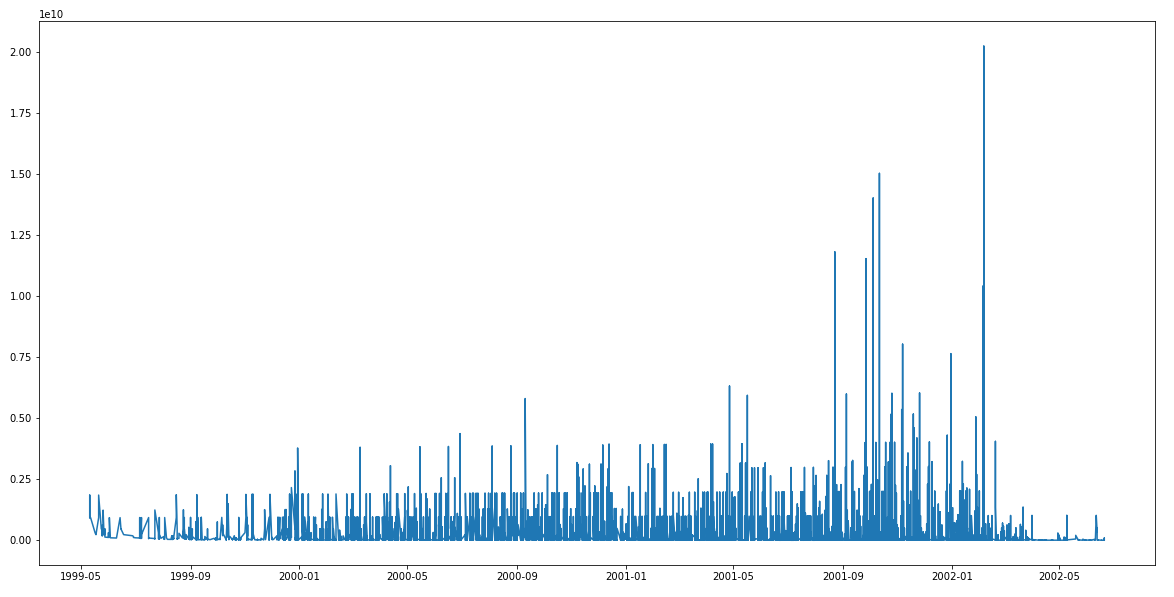
\includegraphics[height=0.6\linewidth,width=\linewidth]{fig/midas/Enron_Anomaly}
	\caption{Der Ausrei�er-Score �ber die Zeit beim ENRON-Datensatz}
	\label{img:midas:enron_anomaly}
\end{figure}



\begin{figure}[H]
	\centering
	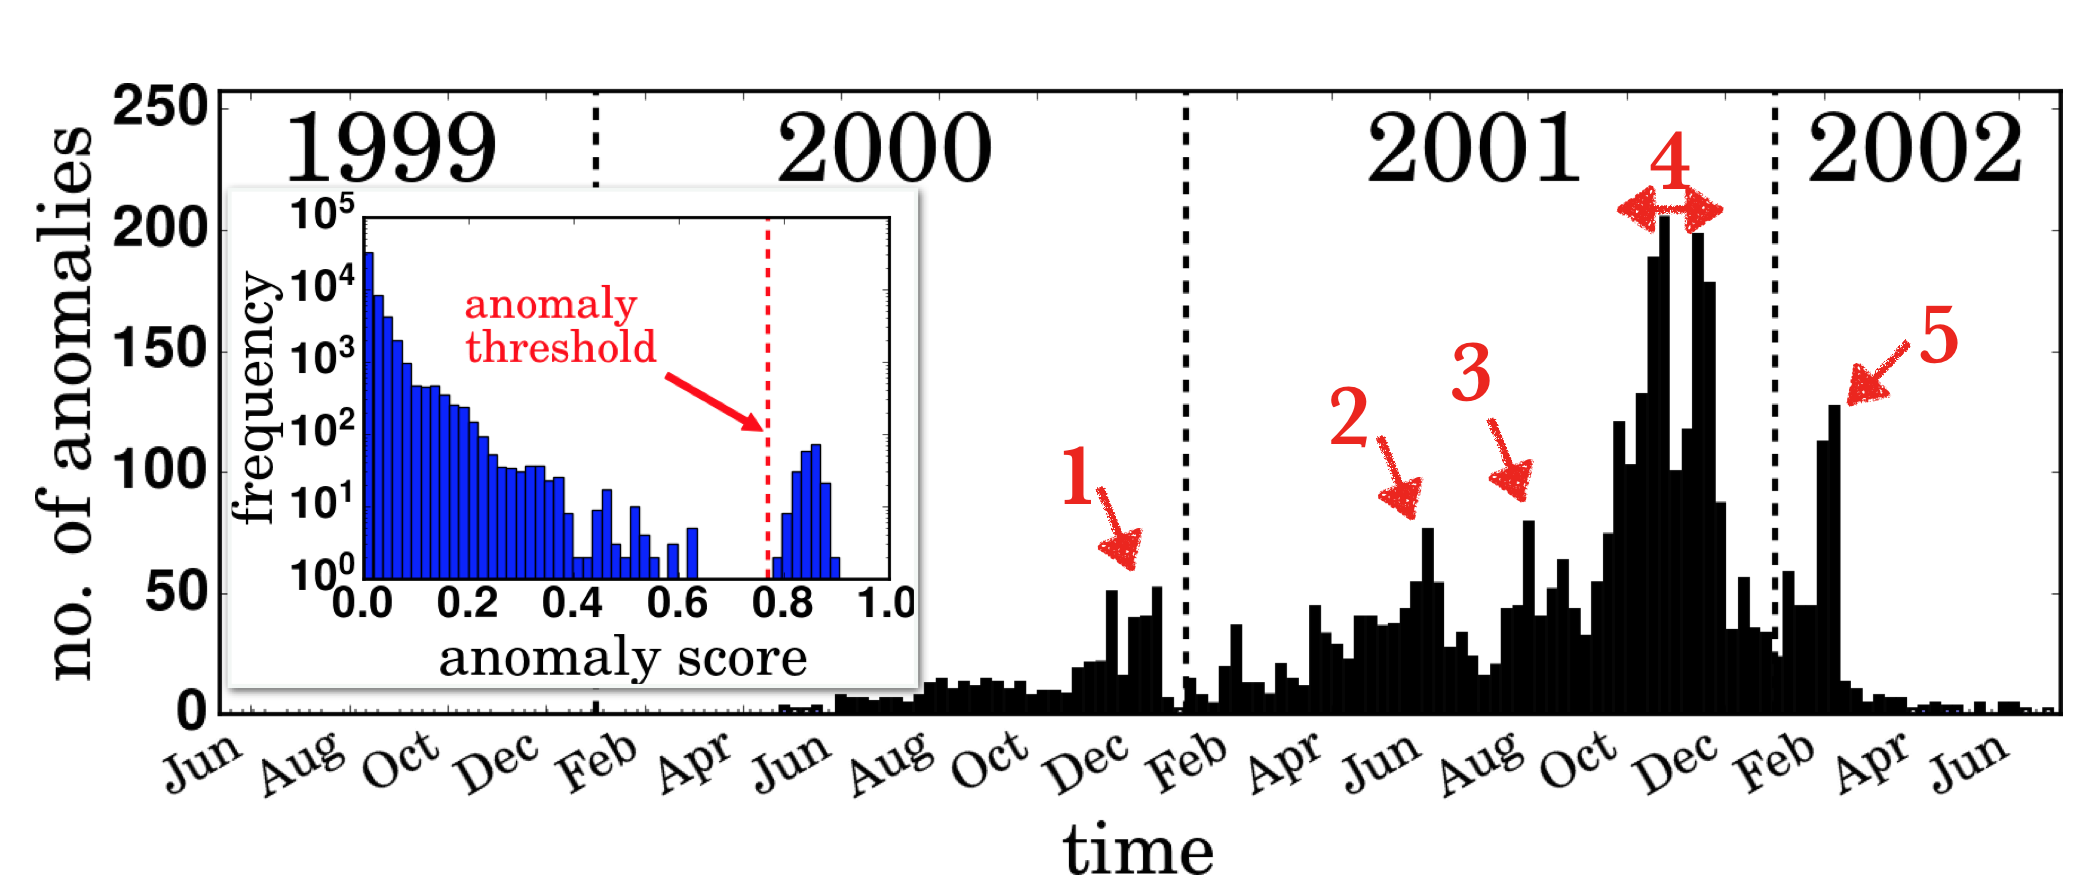
\includegraphics[height=0.4\linewidth,width=\linewidth]{fig/midas/Enron_Label}
	\caption{Die Ausrei�er des SEDANSPOT-Algorithmus}
	\label{img:midas:enron_label}
\end{figure}

Die Herausforderung geeignete \textit{labels} f�r die Datens�tze zu finden wird in zwei Schritten einged�mmt. 

Zum einen werden Erkenntnisse aus dem Schaubild des SEDANSPOT-Algorithmus gewonnen \workTodo{Quelle eingeben}. Hierbei kann man sehen, dass beide Algorithmen einen �hnlichen Verlauf vorweisen. 
Im n�chsten Schritt wird die selbe Vorgehensweise wie aus dem SEDANSPOT-Paper gew�hlt und die ENRON Timeline \workTodo{Quelle einf�gen wie bei Datensatz-Kapitel} zur Erhebung von m�glichen Auswirkungen f�r die Ausrei�er hinzugezogen.

Die \autoref{tab:enrontime} bietet eine �bersicht der historischen Ereignisse, die die Ausrei�er des MIDAS-Algorithmus erkl�ren. Im Vergleich zum SEDANSPOT-Algorithmus werden mehr Ausrei�er erkannt.
  
\begin{table}[h!]
	\centering
    \begin{tabular}{p{0.05\linewidth}|p{0.89\linewidth}}
	\toprule
	1. & Aktie erreicht Allzeithoch. Federal Energy Regulatory Commission ordnet Untersuchung an.\\
	\midrule
	2. & \textbullet Viertelj�hrliche Telefonkonferenz zur Finanzsituation und erste Symptome eines Problems. \newline \textbullet \enquote{Geheimes} Treffen -- Schwarzenegger, Lay, Milken. Angebot zur Rettung der Deregulierung. \\
	\midrule
	3. & \textbullet Skilling (CEO) k�ndigt. Mitarbeiterin warnt Lay (Gr�nder) vor Pleite. Skilling verkauft seine Aktien. \newline \textbullet Enron ver�ffentlicht 618 Mio. \$ Verlust. Interessenskonflikt wird untersucht und Akten vernichtet. \\
	\midrule
	4. & \textbullet Beginn der Strafermittlung. Lay's R�cktritt \newline \textbullet Internen Ermittlung verteilt die Schuld auf F�hrungskr�fte und den Vorstand \\
	\bottomrule
\end{tabular}
	\caption{�bersicht �ber historische Ereignisse, die den Ausrei�ern zuzuordnen sind}
	\label{tab:enrontime}
\end{table}




\begin{figure}[H]
	\centering
	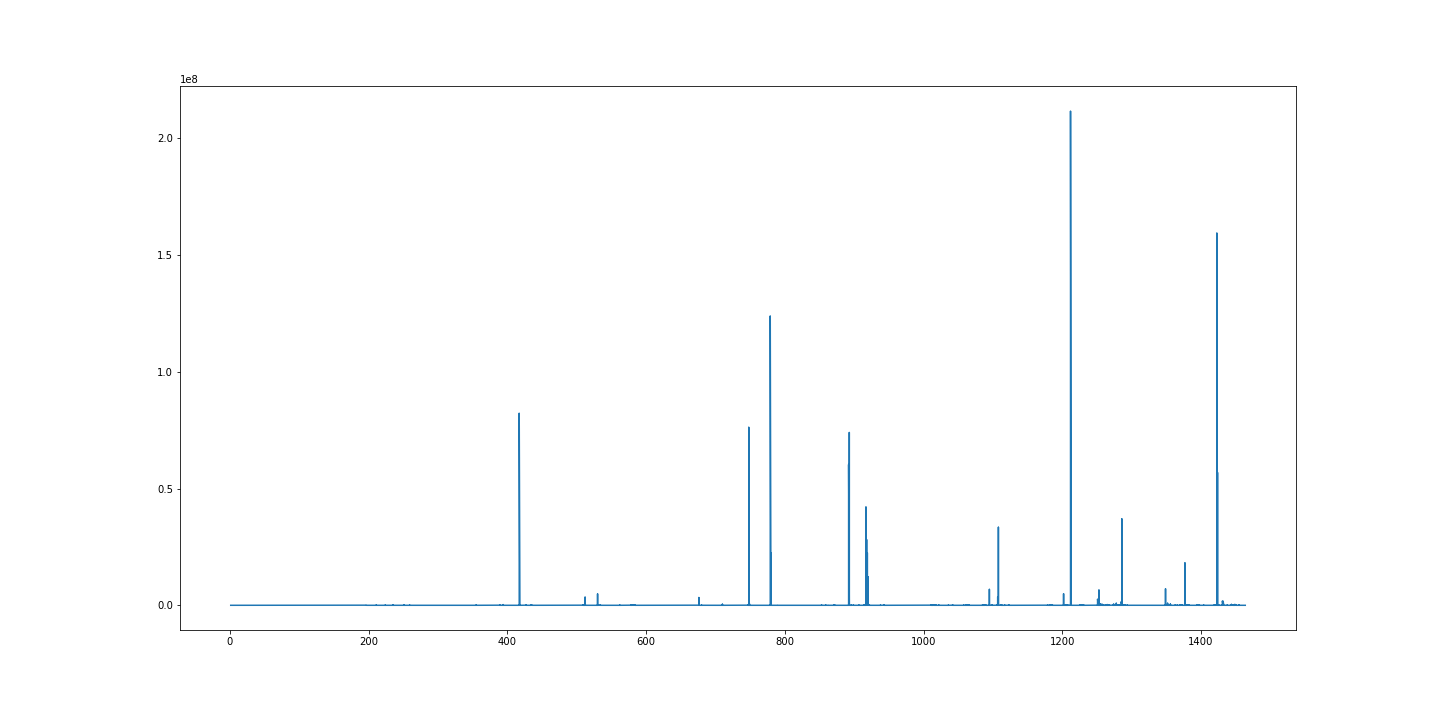
\includegraphics[height=0.6\linewidth,width=\linewidth]{fig/midas/Darpa_Anomaly}
	\caption{Der Ausrei�er-Score �ber die Zeit beim DARPA-Datensatz}
	\label{img:midas:darpa_anomaly}
\end{figure}

Bei der Anwendung des MIDAS auf dem DARPA-Datensatz sieht man sehr sch�n einzelne Ausrei�er, die entdeckt wurden. F�r diesen Datensatz gibt es, speziell f�r MIDAS entwickelt, einen \textit{ground truth}, der die \textit{labels} f�r diesen Datensatz zur Verf�gung stellt.

Bei der Berechnung der \dq Area under the Curve \dq\space f�r die ermittelten Ausrei�er-Scores wird ein Wert von $0.9172724836793507$ berechnet. Das bedeutet, dass der MIDAS-Algorithmus mit einer Wahrscheinlichkeit von ca. 91,73\% die Kanten des Datensatzes richtig klassifiziert.  

Somit kann festgehalten werden, dass MIDAS ein sehr guter Algorithmus ist bei der Erkennung von Ausrei�ern in Graphen und eine sehr hohe Genauigkeit erreicht.

\workTodo{Schwierigkeit geeignete Datens�tze zu finden, dazu gibt es ein Paper. Wenn man die Anomalyscores als gewichte nimmt, kommen Graphen in Networkx raus in denen man die anomalous nodes identifizieren kann dabei sollten es Edges sein}


\section{Ausrei�er-Erkennung in Zeitreihen}
\label{sec:resultsOTs}
\workTodo{Tabelle wie f�r Netsimile einf�gen bzgl. den verschiedenen Numenta-Datens�tzen. Bisher nicht dringlich gewesen, da MIDAS schlecht ist und wir das f�r den abstract nicht ben�tigen}

Um den MIDAS Algorithmus auf Zeitreihen anwenden zu k�nnen muss die Zeitreihe, wie in \autoref{chap:trsnsMidas} beschrieben, zun�chst in verschiedene Netzwerke umgewandelt werden. Bei den Tests konnte festgestellt werden, dass der MIDAS Algorithmus nicht dazu in der Lage ist Ausrei�er in Zeitreihen zu erkennen. Die vollst�ndigen Ergebnisse der Tests k�nnen in \autoref{chap:appendix_midas_ts} eingesehen werden. Hierbei ist jedoch der Verlauf des Ausrei�er Scores schwierig zu interpretieren. Es ist zu erkennen, das der Ausrei�er-Score zu Beginn eines jeden Abschnitts sehr hoch ist, am Ende des Abschnitts ist der Ausrei�er Score hingegen relativ niedrig. Grund hierf�r ist, das die Anzahl an Kanten zu Beginn eines Abschnittes im Verh�ltnis zu der Anzahl an Kanten aus den vorangegangenen Abschnitten deutlich niedriger ist. Im weiteren Verlauf werden weitere Kanten innerhalb des Abschnitts hinzugef�gt. Dadurch gleicht sich die Anzahl an Kanten innerhalb der Abschnitte an und der Ausrei�er Score sinkt.

Der MIDAS Algorithmus ist lediglich bei einer Zeitreihe dazu in der Lage den Ausrei�er zu identifizieren. Hierbei handelt es sich um die Zeitreihe mit erh�hter Amplitude (vgl. \autoref{img:midasTSresultJumpsup}). Durch den Ausschlag nach oben in der Zeitreihe entsteht ein Netzwerk, mit sehr hohen Gewichten. Die hohen Gewichte f�hren zu einer erh�hten Anzahl an Kanten, was schlussendlich zu einem Ausschlag des Ausrei�er Scores f�hrt. Die erh�hte Anzahl an Kanten f�hrt ebenfalls dazu das der Abschnitt mit dem Ausrei�er in der Abbildung deutlich breiter ist als die anderen. Bei anderen Ausrei�er Typen sind die Differenzen zwischen den verschiedenen Elementen der Zeitreihe nicht so gro�. Dadurch ergeben sich keinerlei hohe Kantengewichte und der Ausrei�er kann nicht erkannt werden.


\begin{figure}[h]
	\centering
	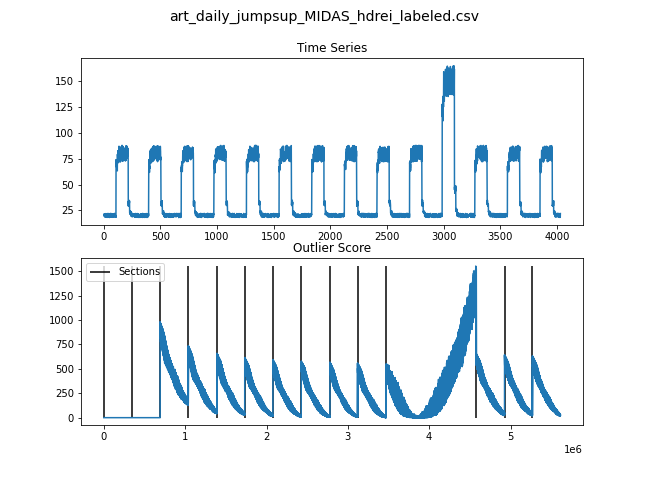
\includegraphics[width=0.5\textwidth]{fig/resultsMidasTS/art_daily_jumpsup_MIDAS_hdrei_labeled_result.png}
	\caption{MIDAS Algorithmus angewandt auf Zeitreihe mit einer erh�ten Amplitude.}
	\label{img:midasTSresultJumpsup}
\end{figure}

Teilweise f�hren die Ausrei�er auch zu besonders wenigen Kanten (vgl. \autoref{img:midasTSresultsFlatSeqChange}). Bei diesem Ausrei�er Typ sind alle Werte auf der selben Ebene. Dadurch gehen die Kantengewichte gegen Null. Dies f�hrt zu einem sehr kurzen Abschnitt in der Abbildung (Der Abschnitt wurde mit einem Pfeil markiert). \workTodo{Noch Pfeil in Graphik einf�gen} Des weiteren ergibt sich durch die Ausrei�er eine leicht ver�nderte Anzahl an Kanten in dem Abschnitt mit dem Ausrei�er (vgl. \autoref{img:midasTSresultsFlatSeqChange}). Die Abweichungen sind jedoch so gering, dass es nicht zu einem starken Anstieg des Ausrei�er Scores f�hrt.
\label{sec:resultTSwithoutMidas}

\begin{figure}[h]
	\centering
	\subfloat[Zeitreihe mit Zyklus Aussetzter]{
		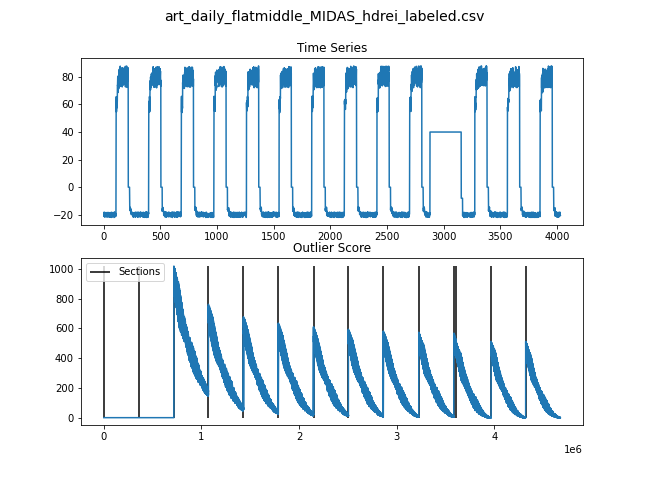
\includegraphics[width=0.5\textwidth]{fig/resultsMidasTS/art_daily_flatmiddle_MIDAS_hdrei_labeled_result.png}}
	\subfloat[Zeitreihe mit Frequenz�nderung]{
		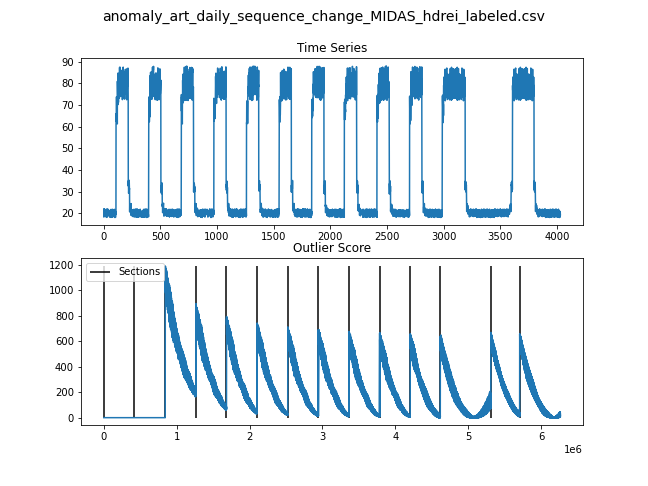
\includegraphics[width=0.5\textwidth]{fig/resultsMidasTS/anomaly_art_daily_sequence_change_MIDAS_hdrei_labeled_result.png}}
	\caption{Ausrei�er Erkennung in Zeitreihen MIDAS Algorithmus}
	\label{img:midasTSresultsFlatSeqChange}
\end{figure}

Es wurden au�erdem Tests durchgef�hrt um zu Untersuchen, wie sich der Algorithmus bei ver�nderter Fenstergr��e verh�lt (vgl. \autoref{img:midasTSresults110}). Bei den Untersuchungen in \autoref{img:midasTSresultJumpsup} und \autoref{img:midasTSresultsFlatSeqChange} wurde einer Fenstergr��e von 288 genutzt, was der Saisonalit�t der Zeitreihe entspricht. F�r dieses Experiment wurde einer Fenstergr��e von 110 verwendet. Es konnte festgestellt werden, das diese Ver�nderung keinen zus�tzlichen Nutzen erbringt. Allerdings ist der Ausschlag nach oben im Ausrei�er Score f�r die Zeitreihe mit erh�hter Amplitude noch deutlicher zu erkennen. Die anderen Ausrei�er Typen werden weiterhin nicht erkannt.

\begin{figure}[h]
	\centering
	\subfloat[Zeitreihe mit einer Frequenz�nderung]{
		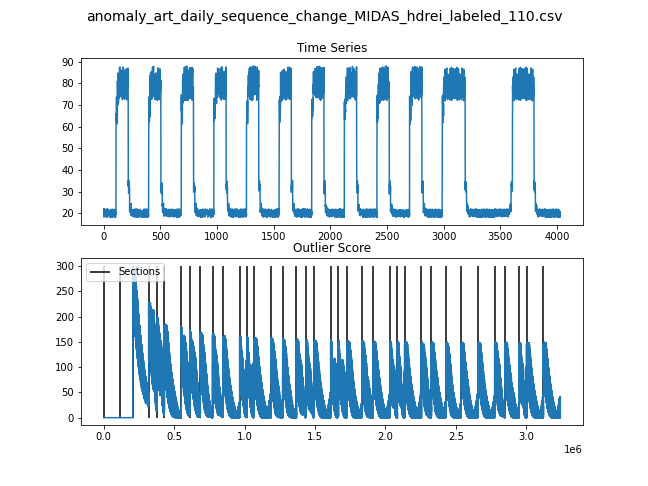
\includegraphics[width=0.5\textwidth]{fig/resultsMidasTS/anomaly_art_daily_sequence_change_MIDAS_hdrei_labeled_110_result.png}}	
	\subfloat[Zeitreihe mit erh�hter Amplitude]{
		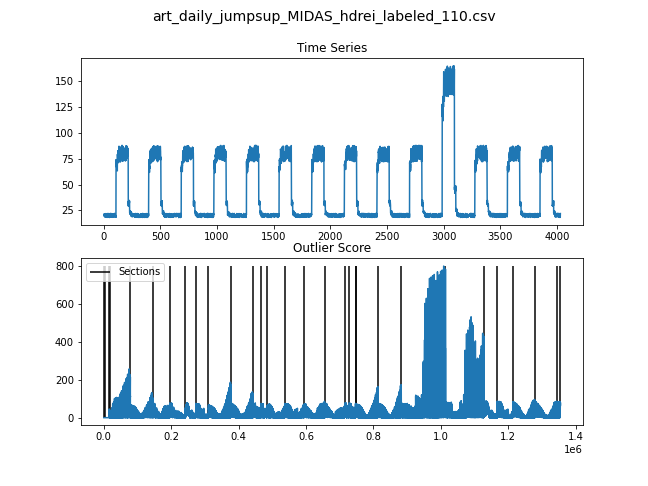
\includegraphics[width=0.5\textwidth]{fig/resultsMidasTS/art_daily_jumpsup_MIDAS_hdrei_labeled_110_result.png}}
	\caption{Ausrei�er Erkennung Zeitreihen MIDAS Algorithmus Fenstergr��e 110}
	\label{img:midasTSresults110}
\end{figure}

In einem n�chsten Schritt wurde untersucht inwiefern der MIDAS-R Algorithmus zu einer Verbesserung bei der Ausrei�er Erkennung beitragen kann (vgl. \autoref{img:midasRTSresults}). Der MIDAS-R Algorithmus ber�cksichtigt bei der Berechnung des Ausrei�er Scores f�r den aktuellen Abschnitt auch die Daten aus der j�ngsten Vergangenheit(vorangegangene Abschnitte). Aus diesem Grund erhofften wir uns durch den Einsatz des MIDAS-R Algorithmus, dass die Ausschl�ge zu beginn eines jeden Abschnitts aus bleiben, sodass Ausrei�er deutlicher hervortreten. Es konnte festgestellt werden, dass der Ausschlag des Ausrei�er Scores zu Beginn der Abschnitte deutlich kleiner ist. Jedoch steigt der Ausrei�er Score zum Ende eines jeden Abschnitts wieder an. Es konnte somit keine Signifikante Verbesserung bei der Erkennung von Ausrei�ern erreicht werden. Insbesondere da der MIDAS-R Algorithmus ebenfalls nur den Ausrei�er in der Zeitreihe mit erh�hter Amplitude anzeigt. Somit konnte festgestellt werden, dass auch die durch den MIDAS-R Algorithmus eingef�hrten Features zu keiner Verbesserung der Ergebnisse gef�hrt haben. 
\workTodo{Vielleicht k�nnte eine Verbesserung erreicht werden wenn andere Features eingef�hrt werden w�rden.}


\begin{figure}[h]
	\centering
	\subfloat[Zeitreihe mit geringerer Amplitude]{
		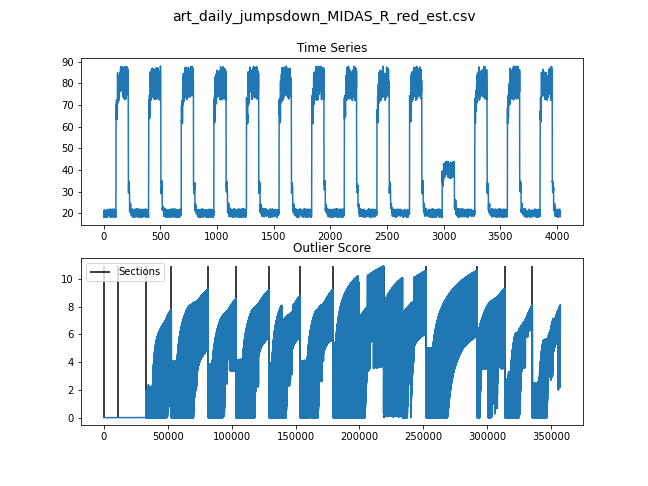
\includegraphics[width=0.5\textwidth]{fig/reultsMidasR/art_daily_jumpsdown_MIDAS_R_red_est_result}}
	\subfloat[Zeitreihe mit erh�hter Amplitude]{
		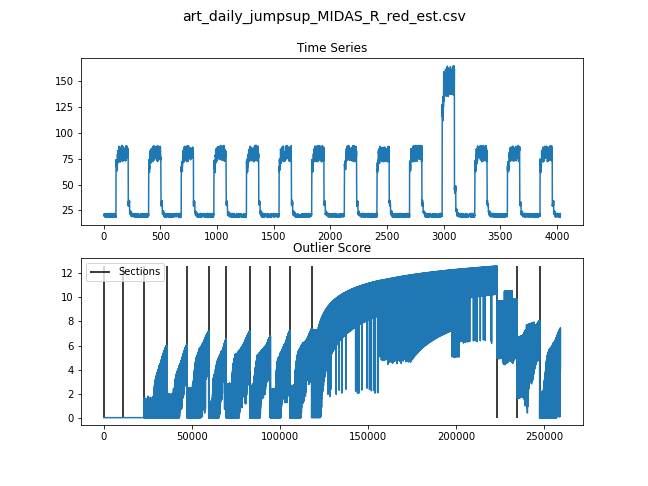
\includegraphics[width=0.5\textwidth]{fig/reultsMidasR/art_daily_jumpsup_MIDAS_R_red_est_result}}
	\caption{Ausrei�er Erkennung Zeitreihen MIDAS-R}
	\label{img:midasRTSresults}
\end{figure}



\chapter{Fazit und Ausblick}
\label{chap:fua}

\section{Fazit}
\label{sec:fua-f}

Die Erkenntnisse und Ergebnisse des Forschungsprojekts zeigen deutlich, dass graphen-basierte Algorithmen erfolgreich auf Zeitreihendaten angewendet werden k�nnen. Im Speziellen dynamische Algorithmen erzielen eine qualitative Erkennung von verschiedensten Ausrei�ertypen. Zudem ber�cksichtigen diese graphen-basierte Algorithmen den Faktor Zeit, der essentiell f�r diesen Datentyp ist.
Inbesondere der NetSimile-Algorithmus hat, nach Optimierung, die Anforderungen des Forschungsprojekts erf�llt. Dieser Algorithmus ist dynamisch, multidimensional, performant und die Erkennung von Ausrei�ern in Zeitreihen ist sehr gut. Der Schwerpunkt hierbei liegt bei der Wahl der richtigen Features. Strukturelle Merkmale sind eher ungeeignet bei vollst�ndig verkn�pften Graphen und sollten ersetzt werden durch Features, wie bspw. die Gewichtung der Kanten. 

%\workTodo{Tabelle in den Anhang}
%\begin{table}[h!]
%	\centering
%	\begin{tabular}{P{0.3\linewidth}|P{0.31\linewidth}|P{0.31\linewidth}}
%		\toprule
%		& \textbf{Netsimile} & \textbf{MIDAS} \\
%		\midrule
%		AmpRise & 54 min 32 sec & 05 min 26 sec \\
%		\midrule
%		Drift & 57 min 29 sec & 05 min 22 sec \\
%		\midrule
%		Flatmiddle & 62 min 50 sec & 06 min 01 sec \\
%		\midrule
%		Increase Noise & 51 min 56 sec & 05 min 40 sec \\
%		\midrule
%		Jumps Down & 51 min 30 sec & 05 min 53 sec \\
%		\midrule
%		Jumps Up & 50 min 40 sec & 05 min 12 sec \\
%		\midrule
%		No Jump & 65 min 45 sec & 06 min 01 sec \\
%		\midrule
%		Peaks & 61 min 31 sec & 05 min 55 sec \\
%		\midrule
%		Sequence Change & 49 min 53 sec & 06 min 41 sec \\
%		\midrule
%		Darpa & 185 min 49 sec & 05 min 29 sec \\
%		\midrule
%		Enron & 01 min 47 sec & 05 min 14 sec \\
%		\bottomrule
%	\end{tabular}
%	\caption{�berblick der Performanz in [min]}
%	\label{tab:performance}
%\end{table}



\section{Ausblick}
\label{sec:fua-a}

Im Rahmen des Forschungsprojekts wurden drei Thematiken behandelt. Zun�chst einmal wurde eine M�glichkeit ermittelt Zeitreihendaten in einen Graphen umzuwandeln. In einem weiteren Schritt wurden graphen-basierte Algorithmen auf die transformierten Zeitreihendaten angewandt. Im Anschluss wurden diese Algorithmen hinsichtlich ihrer Eignung zur Ausrei�ererkennung verglichen.

Durch die erfolgreiche Transformation von Zeitreihendaten in Graphen kann der Vorgang ebenso f�r andere Datenkategorien herangezogen werden, unter der Pr�misse, dass Distanzen zwischen den einzelnen Elementen des Datensatzes gebildet werden k�nnen. So ist es im n�chsten Schritt m�glich bspw. Ausrei�er in Finanzdaten oder Bilddaten zu erkennen. 

Der NetSimile-Algorithmus kann durch neue Merkmale erg�nzt werden. So ist es zuk�nftig m�glich neben den mathematischen Merkmalen auch statistische Algorithmen als Feature einzusetzen um eine erweiterte und optimierte M�glichkeit zu erhalten Aussagen hinsichtlich Ausrei�er treffen zu k�nnen. Eine heutige Problematik des NetSimile ist zum einen die, dass er nur den Ausrei�er-Graphen zur�ckgibt und zum anderen wird der Graph erst dann berechnet, wenn dieser alle Kanten eines Zeitintervalls beinhaltet. Hierbei k�nnen weitere Optimierungen folgen, die bspw. den Ausrei�er-Graphen auf Knoten oder Kanten untersucht, die f�r den Ausrei�er-Score am relevantesten sind. Zudem kann eine Methode ermittelt werden, die einen Graphen iterativ vergr��ert, damit eventuell schon vor dem vollst�ndigen Berechnen des Graphs bestimmt werden kann, ob es sich um einen Ausrei�er handelt. Zuletzt kann der NetSimile so erweitert werden, dass er in Echtzeit Ausrei�er, bspw. im IoT- oder Industrie 4.0-Umfeld, entdeckt. 


%\textit{Aufschrieb}
%Der NetSimile Algorithmus wurde bisher nur auf Zeitreihendaten und Graphen angewendet. Interessant w�ren hierbei ebenso Bilddaten, biologische Daten und andere Netzwerke. Die einzige Voraussetzung ist die Berechnung einer Distanz zwischen einzelnen Elementen in diesen Daten. Zudem gibt es viele statische Algorithmen, die dem NetSimile als Feature hinzugef�gt werden k�nnen. Erkennt der Perculation Algorithmus bspw. Ausrei�er-Typen wie Increase-noise, Jumpsdown, Jumpsup und Flatmiddle, so kann nach weiteren Algorithmen gesucht werden, die die anderen Ausrei�er Typen erkennen. Zudem wird beim NetSimile Algorithmus lediglich der Graph zur�ckgegeben der als Ausrei�er identifiziert wurde, nicht aber der Grund daf�r. Hierf�r k�nnten weitere Untersuchungen durchgef�hrt werden, wie bspw. die Analyse der Features, welches sich am meisten von den anderen unterschieden hat oder einer anschlie�enden Analyse durch den Oddball Algorithmus, welche die Anomalien innerhalb des Graphens untersucht. 
%
%\workTodo{eventuell andere Distanzma�e zur Transformierung hinzuziehen? Da wir so auf den ersten Punkt genauer eingehen w�rden}
%Eine weitere Optimierung, die durchgef�hrt werden kann, ist die Verwendung anderer Distanzma�e. Hierbei kann die Eignung verschiedener Distanzen f�r spezifische Anwendungsf�lle analysiert werden. Die Validierung der Distanzma�e kann durch vorhandene Datens�tze erfolgen. Ebenso ist es m�glich synthetische Referenzdatens�tze zu erstellen, die spezifische Muster bzw. Daten sowie entsprechende Labels beinhalten. Durch die Verwendung dieser Datens�tze ist die Validierung des NetSimile Algorithmus f�r weitere Anwendungsf�lle m�glich.
%
%Des weiteren k�nnte eine allgemeine Forschung gestartet werden, welche untersucht, welche Features f�r spezifische Anwendungsgebiete geeignet sein k�nnten. 
%
%
%\workTodo{Ausblick schreiben}

\appendix
\newpage
\chapter{Netsimile}
\section{Eindimensionales Signal}
\begin{figure}
	\centering
	\subfloat[Caption for sub-figure1]{
		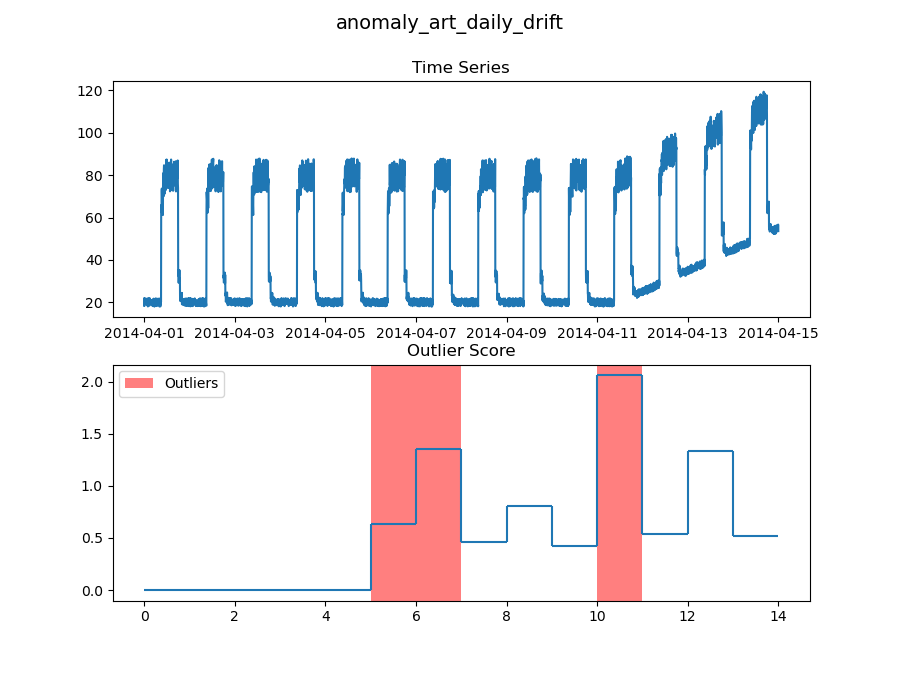
\includegraphics[width=0.5\textwidth]{fig/resultsNetismile/1D/anomaly_art_daily_drift}}
	\subfloat[Caption for sub-figure1]{
		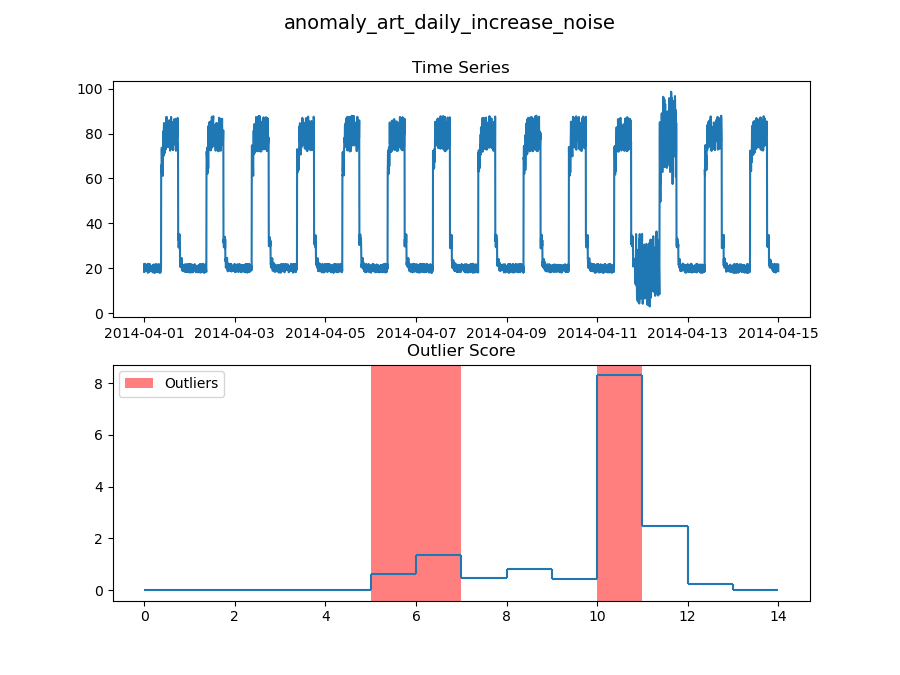
\includegraphics[width=0.5\textwidth]{fig/resultsNetismile/1D/anomaly_art_daily_increase_noise}}
	\qquad
	\subfloat[Caption for sub-figure1]{
		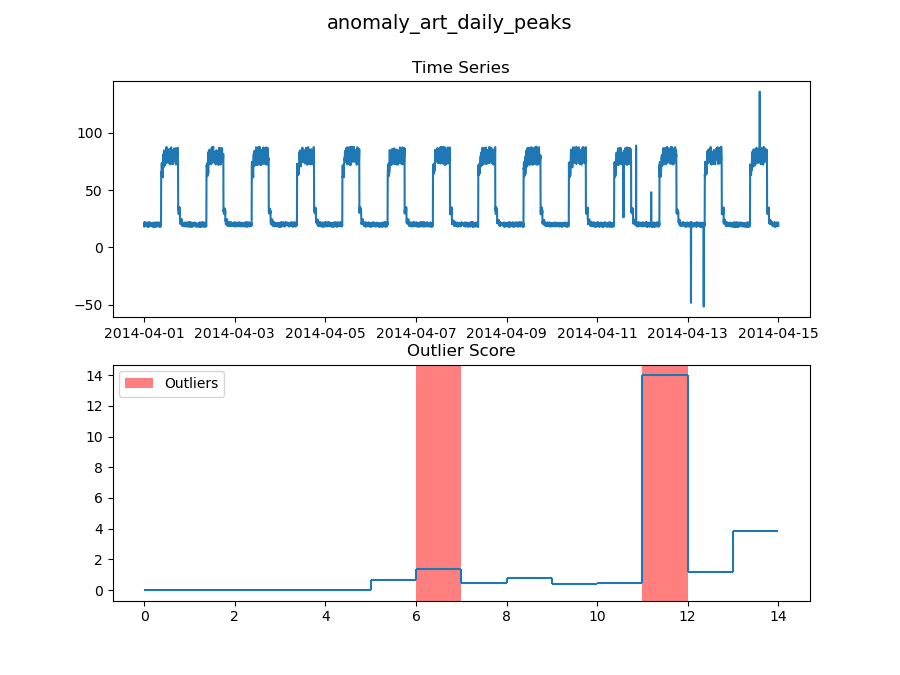
\includegraphics[width=0.5\textwidth]{fig/resultsNetismile/1D/anomaly_art_daily_peaks}}
	\subfloat[Caption for sub-figure1]{
		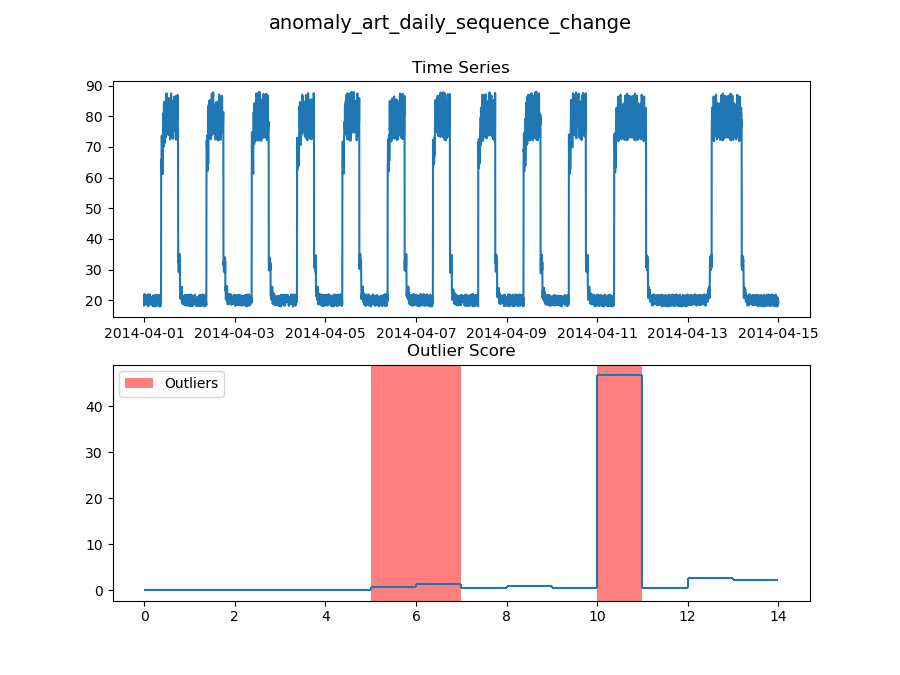
\includegraphics[width=0.5\textwidth]{fig/resultsNetismile/1D/anomaly_art_daily_sequece_change}}
	\qquad
	\label{img:isomappictures1}
\end{figure}
\begin{figure}\ContinuedFloat
	\subfloat[Caption for sub-figure1]{
		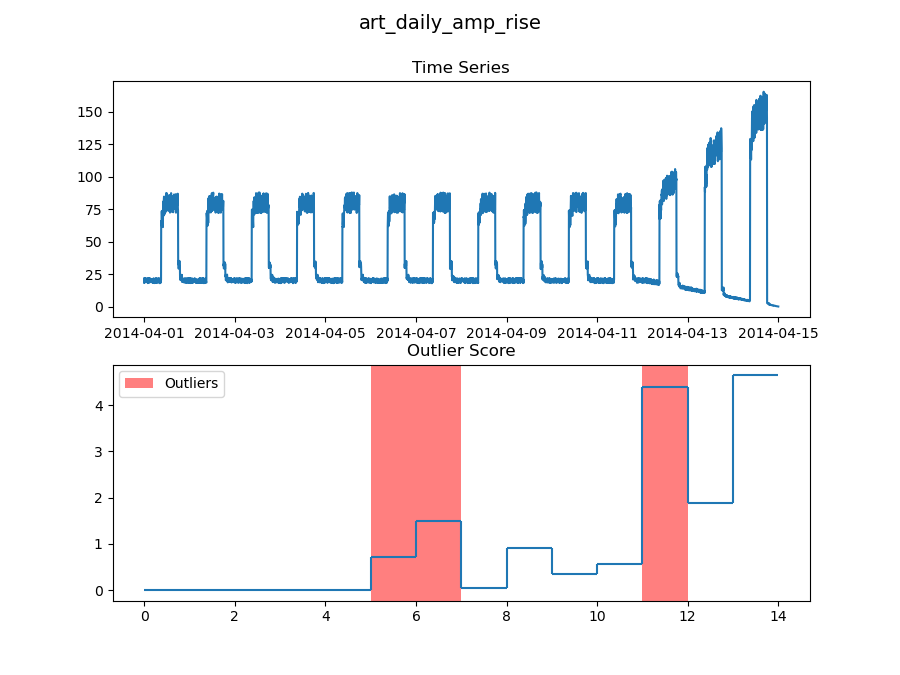
\includegraphics[width=0.5\textwidth]{fig/resultsNetismile/1D/art_daily_amp_rise}}
	\subfloat[Caption for sub-figure1]{
		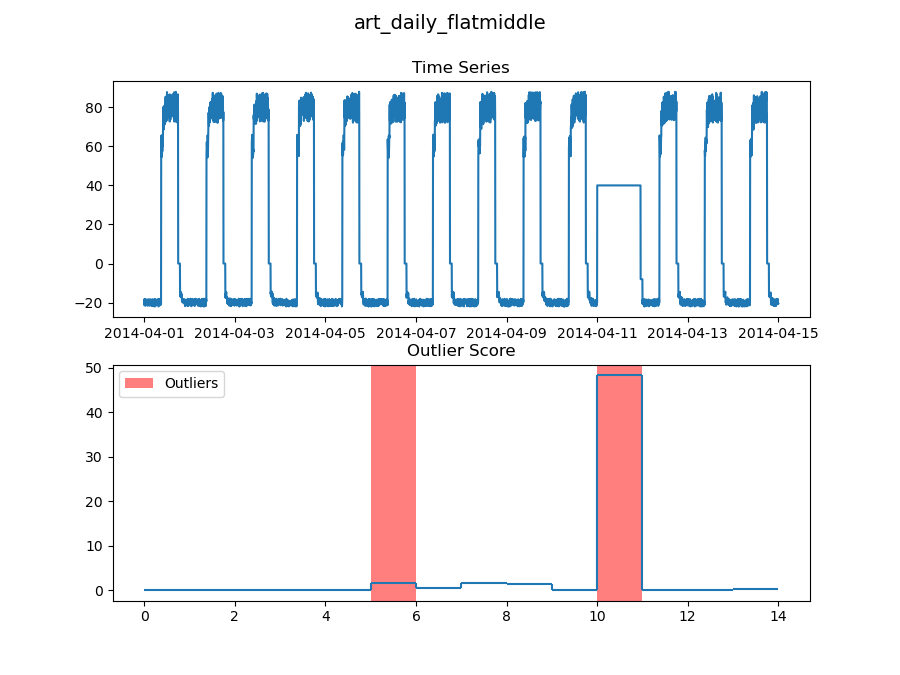
\includegraphics[width=0.5\textwidth]{fig/resultsNetismile/1D/art_daily_flatmiddle}}
	\qquad
	\subfloat[Caption for sub-figure1]{
		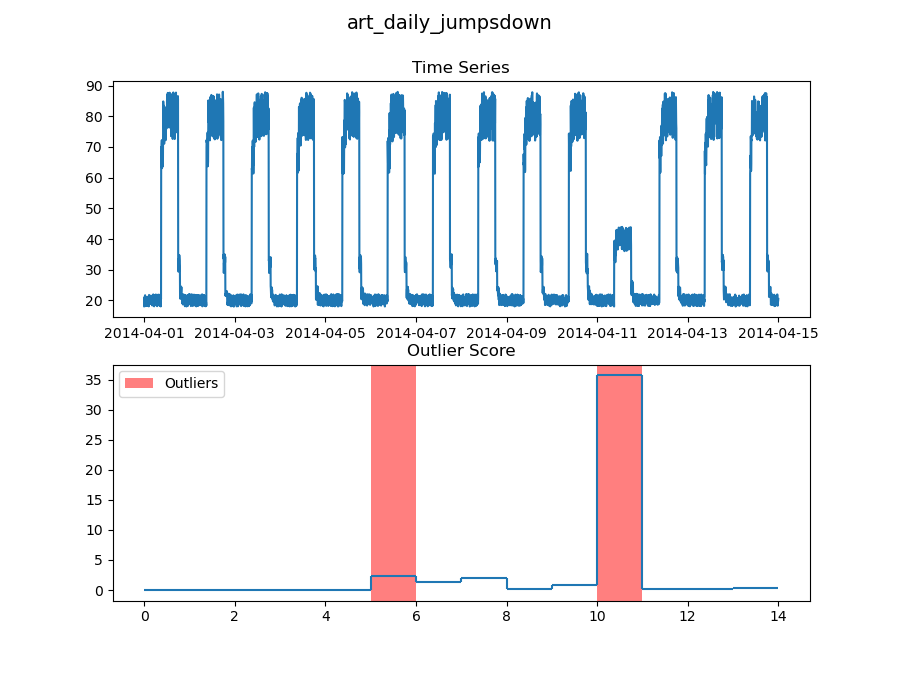
\includegraphics[width=0.5\textwidth]{fig/resultsNetismile/1D/art_daily_jumpsdown}}
	\subfloat[Caption for sub-figure1]{
		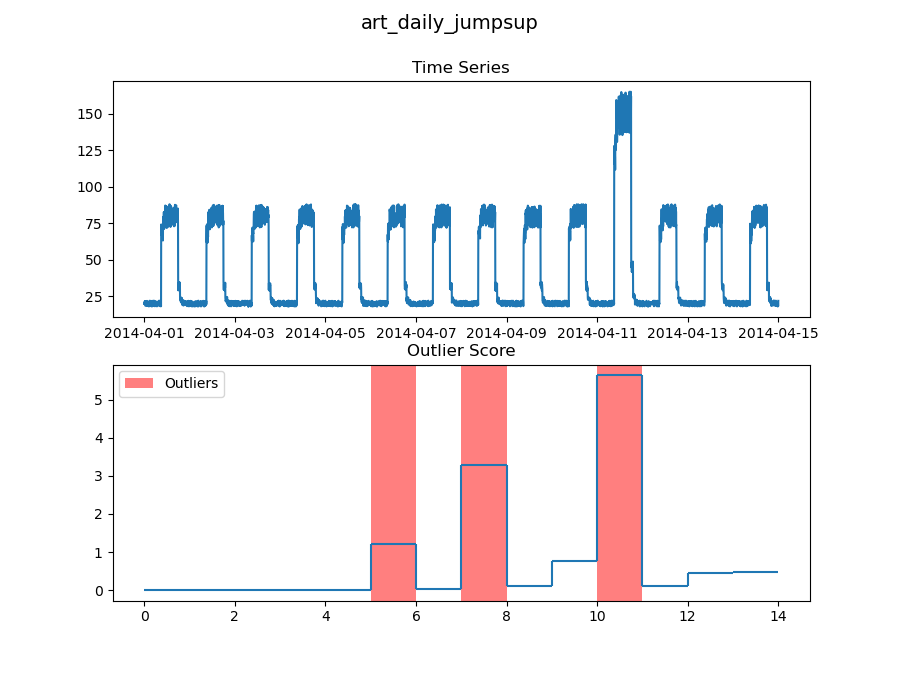
\includegraphics[width=0.5\textwidth]{fig/resultsNetismile/1D/art_daily_jumpsup}}
	\qquad
	\subfloat[Caption for sub-figure1]{
		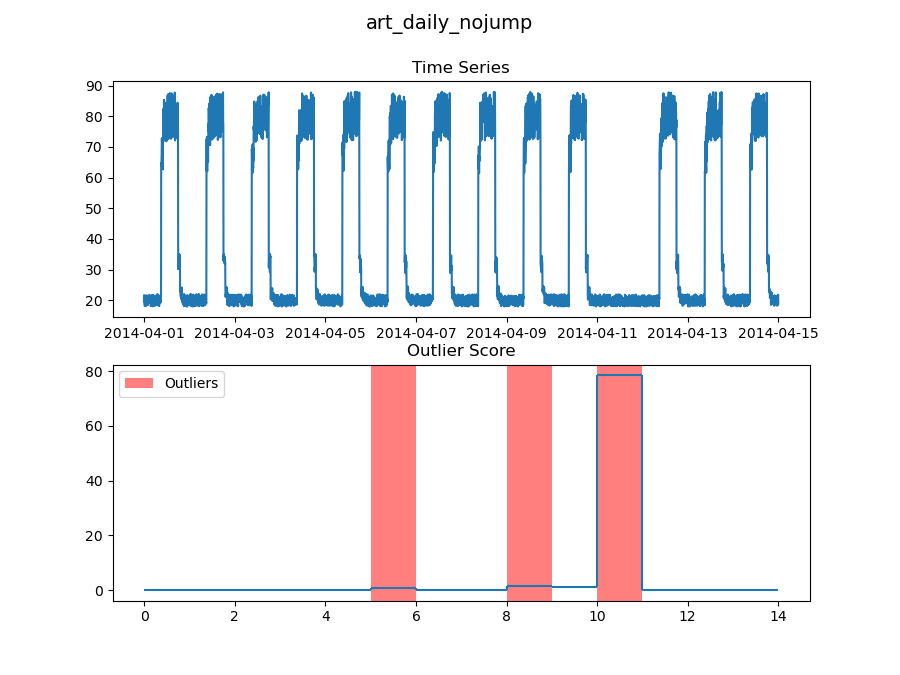
\includegraphics[width=0.5\textwidth]{fig/resultsNetismile/1D/art_daily_nojump}}
	\label{img:isomappictures2}
\end{figure}

\workTodo{Wrong picture for daily peaks. Change that the sixed element is not always an outlier}

\newpage
\section{Zweidimensionales Signal}
\begin{figure}
	\centering
	\subfloat[Caption for sub-figure1]{
		\includegraphics[width=0.5\textwidth]{fig/resultsNetismile/2D/anomaly_art_daily_drift}}
	\subfloat[Caption for sub-figure1]{
		\includegraphics[width=0.5\textwidth]{fig/resultsNetismile/2D/anomaly_art_daily_increase_noise}}
	\qquad
	\subfloat[Caption for sub-figure1]{
		\includegraphics[width=0.5\textwidth]{fig/resultsNetismile/2D/anomaly_art_daily_peaks}}
	\subfloat[Caption for sub-figure1]{
		\includegraphics[width=0.5\textwidth]{fig/resultsNetismile/2D/anomaly_art_daily_sequence_change}}
	\qquad
	\label{img:isomappictures1}
\end{figure}
\begin{figure}\ContinuedFloat
	\subfloat[Caption for sub-figure1]{
		\includegraphics[width=0.5\textwidth]{fig/resultsNetismile/2D/art_daily_amp_rise}}
	\subfloat[Caption for sub-figure1]{
		\includegraphics[width=0.5\textwidth]{fig/resultsNetismile/2D/art_daily_flatmiddle}}
	\qquad
	\subfloat[Caption for sub-figure1]{
		\includegraphics[width=0.5\textwidth]{fig/resultsNetismile/2D/art_daily_jumpsdown}}
	\subfloat[Caption for sub-figure1]{
		\includegraphics[width=0.5\textwidth]{fig/resultsNetismile/2D/art_daily_jumpsup}}
	\qquad
	\subfloat[Caption for sub-figure1]{
		\includegraphics[width=0.5\textwidth]{fig/resultsNetismile/2D/art_daily_nojump}}
	\label{img:isomappictures2}
\end{figure}


\workTodo{Wrong picture for daily peaks. Change that the sixed element is not always an outlier}
\newpage
\chapter{Midas}
\subsubsection{Eindimensionales Signal}
\label{chap:appendix_midas_ts}
\begin{figure}[h]
	\centering
	\subfloat[Ausrei�er-Typ Signal Drift\label{img:dailyDriftIso}]{
		\includegraphics[width=0.5\textwidth]{fig/resultsMidasTS/anomaly_art_daily_drift_MIDAS_hdrei_labeled_result}}
	\subfloat[Ausrei�er-Typ Zunahme an Rauschen\label{img:increaseNoiseIso}]{
		\includegraphics[width=0.5\textwidth]{fig/resultsMidasTS/anomaly_art_daily_increase_noise_MIDAS_hdrei_labeled_result}}
	\qquad
	\subfloat[Ausrei�er-Typ Einzelne Peaks\label{img:dailyPeaksIso}]{
		\includegraphics[width=0.5\textwidth]{fig/resultsMidasTS/anomaly_art_daily_peaks_MIDAS_hdrei_labeled_result}}
	\subfloat[Ausrei�er-Typ Frequenz�nderung\label{img:sequenceChangeIso}]{
		\includegraphics[width=0.5\textwidth]{fig/resultsMidasTS/anomaly_art_daily_sequence_change_MIDAS_hdrei_labeled_result}}
	\qquad
	\label{img:midaspictures1}
\end{figure}
\begin{figure}\ContinuedFloat
	\subfloat[Ausrei�er-Typ Kontinuierliche Zunahme der Amplitude\label{img:ampRiseIso}]{
		\includegraphics[width=0.5\textwidth]{fig/resultsMidasTS/art_daily_amp_rise_MIDAS_hdrei_labeled_result}}
	\subfloat[Ausrei�er-Typ Zyklus-Aussetzer\label{img:flatmiddleIso}]{
		\includegraphics[width=0.5\textwidth]{fig/resultsMidasTS/art_daily_flatmiddle_MIDAS_hdrei_labeled_result}}
	\qquad
	\subfloat[Ausrei�er-Typ Zyklus mit geringerer Amplitude\label{img:jumpsdownIso}]{
		\includegraphics[width=0.5\textwidth]{fig/resultsMidasTS/art_daily_jumpsdown_MIDAS_hdrei_result}}
	\subfloat[Ausrei�er-Typ Zyklus mit h�herer Amplitude\label{img:jumpsupIso}]{
		\includegraphics[width=0.5\textwidth]{fig/resultsMidasTS/art_daily_jumpsup_MIDAS_hdrei_labeled_result}}
	\qquad
	\subfloat[Ausrei�er-Typ Signal-Aussetzer\label{img:nojumpIso}]{
		\includegraphics[width=0.5\textwidth]{fig/resultsMidasTS/art_daily_nojump_MIDAS_hdrei_result}}
	\label{img:midaspictures2}
\end{figure}

\workTodo{Sterne richtig verteilen}
\begin{table}[H]
	\centering
	\begin{tabular}{p{0.42\linewidth}|p{0.37\linewidth}|P{0.15\linewidth}}
		\toprule
		\textbf{Ausrei�ertyp}& \textbf{Dateiname}&
		\textbf{Bewertung}\\
		\midrule
		Einzelne Peaks & anomaly-art-daily-peaks & *\\
		\midrule
		Zunahme an Rauschen & anomaly-art-daily-increase-noise &*\\
		\midrule
		Signal Drift & anomaly-art-daily-drift &** \\
		\midrule
		Kontinuierliche Zunahme der Amplitude& art-daily-amp-rise & **\\
		\midrule
		Zyklus mit h�herer Amplitude & art-daily-jumpsup & *\\
		\midrule
		Zyklus mit geringerer Amplitude & art-daily-jumpsdown & *\\
		\midrule
		Zyklus-Aussetzer & art-daily-flatmiddle &*\\
		\midrule
		Signal-Aussetzer & art-daily-nojump & *\\
		\midrule
		Frequenz�nderung & anomaly-art-daily-sequence-change &*\\
		\bottomrule
	\end{tabular}
	\caption{\centering Bewertung des MIDAS-Algorithmus bzgl. der Erkennung von verschiedenen Ausrei�ertypen in Zeitreihen}
	\label{table:performanceMIDAS}
\end{table}
\newpage
\chapter{Isomap}
\label{app-iso}
\subsubsection{Eindimensionales Signal}
\begin{figure}[h]
	\centering
	\subfloat[Ausrei�ertyp Signal Drift\label{img:dailyDriftIso}]{
		\includegraphics[width=0.5\textwidth]{fig/resultsIsoMap/anomaly_art_daily_drift}}
	\subfloat[Ausrei�ertyp Zunahme an Rauschen\label{img:increaseNoiseIso}]{
		\includegraphics[width=0.5\textwidth]{fig/resultsIsoMap/anomaly_art_daily_increase_noise}}
	\qquad
	\subfloat[Ausrei�ertyp Einzelne Peaks\label{img:dailyPeaksIso}]{
		\includegraphics[width=0.5\textwidth]{fig/resultsIsoMap/anomaly_art_daily_peaks}}
	\subfloat[Ausrei�ertyp Frequenz�nderung\label{img:sequenceChangeIso}]{
		\includegraphics[width=0.5\textwidth]{fig/resultsIsoMap/anomaly_art_daily_sequence_change}}
	\qquad
\end{figure}
\begin{figure}\ContinuedFloat
	\subfloat[Ausrei�ertyp Kontinuierliche Zunahme der Amplitude\label{img:ampRiseIso}]{
		\includegraphics[width=0.5\textwidth]{fig/resultsIsoMap/art_daily_amp_rise}}
	\subfloat[Ausrei�ertyp Zyklus-Aussetzer\label{img:flatmiddleIso}]{
		\includegraphics[width=0.5\textwidth]{fig/resultsIsoMap/art_daily_flatmiddle}}
	\qquad
	\subfloat[Ausrei�ertyp Zyklus mit geringerer Amplitude\label{img:jumpsdownIso}]{
		\includegraphics[width=0.5\textwidth]{fig/resultsIsoMap/art_daily_jumpsdown}}
	\subfloat[Ausrei�ertyp Zyklus mit h�herer Amplitude\label{img:jumpsupIso}]{
		\includegraphics[width=0.5\textwidth]{fig/resultsIsoMap/art_daily_jumpsup}}
	\qquad
	\subfloat[Ausrei�ertyp Signal-Aussetzer\label{img:nojumpIso}]{
		\includegraphics[width=0.5\textwidth]{fig/resultsIsoMap/art_daily_nojump}}
\end{figure}






\newpage
\chapter{Percolation}
\subsubsection{Eindimensionales Signal}
\label{app-perc}
\begin{figure}[h]
	\centering
	\subfloat[Ausrei�ertyp Signal Drift\label{img:dailyDriftPerc}]{
		\includegraphics[width=0.5\textwidth]{fig/resultsPercolation/anomaly_art_daily_drift}}
	\subfloat[Ausrei�ertyp Zunahme an Rauschen\label{img:increaseNoisePerc}]{
		\includegraphics[width=0.5\textwidth]{fig/resultsPercolation/anomaly_art_daily_increase_noise}}
	\qquad
	\subfloat[Ausrei�ertyp Einzelne Peaks\label{img:dailyPeaksPerc}]{
		\includegraphics[width=0.5\textwidth]{fig/resultsPercolation/anomaly_art_daily_peaks}}
	\subfloat[Ausrei�ertyp Frequenz�nderung\label{img:sequenceChangePerc}]{
		\includegraphics[width=0.5\textwidth]{fig/resultsPercolation/anomaly_art_daily_sequence_change}}
	\qquad
	\label{img:isomappictures1}
\end{figure}
\begin{figure}\ContinuedFloat
	\subfloat[Ausrei�ertyp Kontinuierliche Zunahme der Amplitude\label{img:ampRisePerc}]{
		\includegraphics[width=0.5\textwidth]{fig/resultsPercolation/art_daily_amp_rise}}
	\subfloat[Ausrei�ertyp Zyklus-Aussetzer\label{img:flatmiddlePerc}]{
		\includegraphics[width=0.5\textwidth]{fig/resultsPercolation/art_daily_flatmiddle}}
	\qquad
	\subfloat[Ausrei�ertyp Zyklus mit geringerer Amplitude\label{img:jumpsdownPerc}]{
		\includegraphics[width=0.5\textwidth]{fig/resultsPercolation/art_daily_jumpsdown}}
	\subfloat[Ausrei�ertyp Zyklus mit h�herer Amplitude\label{img:jumpsupPerc}]{
		\includegraphics[width=0.5\textwidth]{fig/resultsPercolation/art_daily_jumpsup}}
	\qquad
	\subfloat[Ausrei�ertyp Signal-Aussetzer\label{img:nojumpPerc}]{
		\includegraphics[width=0.5\textwidth]{fig/resultsPercolation/art_daily_nojump}}
	\label{img:isomappictures2}
\end{figure}


\newpage



% % %%%%%% Anhang
%\appendix
%\chapter{OddBall}
\label{chap:a-ob}
\section{Threshold-Ergebnisse}
\label{chap:a-ob-th}
\begin{table}[H]
	\centering
	\includegraphics[width=\textwidth, height=0.72\textheight]{fig/tabelle-threshold-1}
	\caption{Threshold-Ergebnisse}
\end{table}

\section{Local-Outlier-Factor-Ergebnisse}
\label{chap:a-ob-lof}

\begin{table}[H]
\centering
\includegraphics[width=\textwidth]{fig/tabelle-lof-1}
\end{table}

\begin{table}[H]
\centering
\includegraphics[width=\textwidth]{fig/tabelle-lof-2}
\end{table}

\begin{table}[H]
\centering
\includegraphics[width=\textwidth]{fig/tabelle-lof-3}
\end{table}

\begin{table}[H]
\centering
\includegraphics[width=\textwidth]{fig/tabelle-lof-4}
\caption{Local-Outlier-Factor-Ergebnisse}
\end{table}


\section{Local-Outlier-Probability-Ergebnisse}
\label{chap:a-ob-loop}
\begin{table}[H]
	\centering
	\includegraphics[width=\textwidth]{fig/tabelle-loop-1}
\end{table}

\begin{table}[H]
	\centering
	\includegraphics[width=\textwidth]{fig/tabelle-loop-2}
\end{table}

\begin{table}[H]
\centering
\includegraphics[width=\textwidth]{fig/tabelle-loop-3}
\end{table}

\begin{table}[H]
\centering
\includegraphics[width=\textwidth]{fig/tabelle-loop-4}
\end{table}

\begin{table}[H]
\centering
\includegraphics[width=\textwidth]{fig/tabelle-loop-5}
\end{table}

\begin{table}[H]
\centering
\includegraphics[width=\textwidth]{fig/tabelle-loop-6}
\caption{Local-Outlier-Probability-Ergebnisse}
\end{table}

\section{Vergleich LOF und LoOP}
\label{chap:a-ob-lof-loop}

\begin{table}[H]
	\centering
	\includegraphics[width=\textwidth]{fig/tabelle-lof-loop}
	\caption{Vergleich LOF und LoOP}
\end{table}

\section{DBSCAN-Ergebnisse}
\label{chap:a-ob-dbscan}

\begin{table}[H]
	\centering
	\includegraphics[width=\textwidth]{fig/tabelle-dbscan-1}
\end{table}

\begin{table}[H]
\centering
\includegraphics[width=\textwidth]{fig/tabelle-dbscan-2}
\end{table}

\begin{table}[H]
\centering
\includegraphics[width=\textwidth]{fig/tabelle-dbscan-3}
\caption{DBSCAN-Ergebnisse}
\end{table}

\section{DBSCAN+LoOP-Ergebnisse}
\label{chap:a-ob-dbscan-loop}

\begin{table}[H]
	\centering
	\includegraphics[width=\textwidth]{fig/tabelle-dbscan-loop-1}
\end{table}

\begin{table}[H]
\centering
\includegraphics[width=\textwidth]{fig/tabelle-dbscan-loop-4}
\caption{DBSCAN+LoOP-Ergebnisse}
\end{table}

\chapter{SCAN-Ergebnisse}
\label{chap:a-ob-scan}

\begin{table}[H]
	\centering
	\includegraphics[width=\textwidth]{fig/tabelle-scan-1}
\end{table}

\begin{table}[H]
\centering
\includegraphics[width=\textwidth]{fig/tabelle-scan-2}
\end{table}

\begin{table}[H]
\centering
\includegraphics[width=\textwidth]{fig/tabelle-scan-3}
\end{table}

\begin{table}[H]
\centering
\includegraphics[width=\textwidth]{fig/tabelle-scan-4}
\end{table}

\begin{table}[H]
\centering
\includegraphics[width=\textwidth]{fig/tabelle-scan-5}
\end{table}

\begin{table}[H]
\centering
\includegraphics[width=\textwidth]{fig/tabelle-scan-6}
\end{table}

\begin{table}[H]
\centering
\includegraphics[width=\textwidth]{fig/tabelle-scan-7}
\caption{SCAN-Ergebnisse}
\end{table}


\chapter{Random-Walk}
\label{chap:a-rw}
Die nachfolgend aufgelisteten Graphen zeigen die Ergebnisse der Ausrei�er Erkennung mithilfe des Random-Walk Algorithmus. Die Graphen bestehen dabei aus unterschiedlichen Zeitreihen, den identifizierten Ausrei�ern sowie dem Ausrei�er-Score. In den Kapiteln \autoref{chap:a-rw-3D} und \autoref{chap:a-rw-5D} wurden die Dimensionen 2-3 bzw. 2-5 nicht dargestellt, um die �bersichtlichkeit zu gew�hrleisten.

\section{Zweidimensionales Signal}
\label{chap:a-rw-2D}
\begin{figure}[!htbp]
	\centering
	\begin{minipage}[t]{0.45\textwidth}
		\includegraphics[width=\textwidth]{fig/rw-2d-1}
		\caption{Anomalie: Einzelne Peaks}
	\end{minipage}
	\begin{minipage}[t]{0.45\textwidth}
		\includegraphics[width=\textwidth]{fig/rw-2d-2}
		\caption{Anomalie: Zunahme an Rauschen}
	\end{minipage}
\end{figure}

\begin{figure}[!htbp]
	\centering
	\begin{minipage}[t]{0.45\textwidth}
		\includegraphics[width=\textwidth]{fig/rw-2d-3}
		\caption{Anomalie: Signal Drift}
	\end{minipage}
	\begin{minipage}[t]{0.45\textwidth}
		\includegraphics[width=\textwidth]{fig/rw-2d-4}
		\caption{Anomalie: Zunahme der Amplitude}
	\end{minipage}
\end{figure}

\begin{figure}[!htbp]
	\centering
	\begin{minipage}[t]{0.49\textwidth}
		\includegraphics[width=\textwidth]{fig/rw-2d-5}
		\caption{Anomalie: Zyklus mit h�herer Amplitude}
	\end{minipage}
	\begin{minipage}[t]{0.49\textwidth}
		\includegraphics[width=\textwidth]{fig/rw-2d-6}
		\caption{Anomalie: Zyklus mit geringerer Amplitude}
	\end{minipage}
\end{figure}

\begin{figure}[!htbp]
	\centering
	\begin{minipage}[t]{0.49\textwidth}
		\includegraphics[width=\textwidth]{fig/rw-2d-7}
		\caption{Anomalie: Zyklus Aussetzer}
	\end{minipage}
	\begin{minipage}[t]{0.49\textwidth}
		\includegraphics[width=\textwidth]{fig/rw-2d-8}
		\caption{Anomalie: Signal Aussetzer}
	\end{minipage}
\end{figure}

\begin{figure}
	\centering
	\begin{minipage}[t]{0.49\textwidth}
		\includegraphics[width=\textwidth]{fig/rw-2d-9}
		\caption{Anomalie: Frequenz�nderung der Zyklen}
	\end{minipage}
\end{figure}

\section{Dreidimensionales Signal}
\label{chap:a-rw-3D}

\begin{figure}[!htbp]
	\centering
	\begin{minipage}[t]{0.45\textwidth}
		\includegraphics[width=\textwidth]{fig/rw-3d-1}
		\caption{Anomalie: Einzelne Peaks}
	\end{minipage}
	\begin{minipage}[t]{0.45\textwidth}
		\includegraphics[width=\textwidth]{fig/rw-3d-2}
		\caption{Anomalie: Zunahme an Rauschen}
	\end{minipage}
\end{figure}

\begin{figure}[!htbp]
	\centering
	\begin{minipage}[t]{0.45\textwidth}
		\includegraphics[width=\textwidth]{fig/rw-3d-3}
		\caption{Anomalie: Signal Drift}
	\end{minipage}
	\begin{minipage}[t]{0.45\textwidth}
		\includegraphics[width=\textwidth]{fig/rw-3d-4}
		\caption{Anomalie: Zunahme der Amplitude}
	\end{minipage}
\end{figure}

\begin{figure}[!htbp]
	\centering
	\begin{minipage}[t]{0.45\textwidth}
		\includegraphics[width=\textwidth]{fig/rw-3d-5}
		\caption{Anomalie: Zyklus mit h�herer Amplitude}
	\end{minipage}
	\begin{minipage}[t]{0.45\textwidth}
		\includegraphics[width=\textwidth]{fig/rw-3d-6}
		\caption{Anomalie: Zyklus mit geringerer Amplitude}
	\end{minipage}
\end{figure}

\begin{figure}[!htbp]
	\centering
	\begin{minipage}[t]{0.45\textwidth}
		\includegraphics[width=\textwidth]{fig/rw-3d-7}
		\caption{Anomalie: Zyklus-Aussetzer}
	\end{minipage}
	\begin{minipage}[t]{0.45\textwidth}
		\includegraphics[width=\textwidth]{fig/rw-3d-8}
		\caption{Anomalie: Signal-Aussetzer}
	\end{minipage}
\end{figure}

\begin{figure}
	\centering
	\begin{minipage}[t]{0.45\textwidth}
		\includegraphics[width=\textwidth]{fig/rw-3d-9}
		\caption{Anomalie: Frequenz�nderung der Zyklen}
	\end{minipage}
\end{figure}
\newpage

\section{F�nfdimensionales Signal}
\label{chap:a-rw-5D}

\begin{figure}[!htbp]
	\centering
	\begin{minipage}[t]{0.45\textwidth}
		\includegraphics[width=\textwidth]{fig/rw-5d-1}
		\caption{Anomalie: Einzelne Peaks}
	\end{minipage}
	\begin{minipage}[t]{0.45\textwidth}
		\includegraphics[width=\textwidth]{fig/rw-5d-2}
		\caption{Anomalie: Zunahme an Rauschen}
	\end{minipage}
\end{figure}

\begin{figure}[!htbp]
	\centering
	\begin{minipage}[t]{0.45\textwidth}
		\includegraphics[width=\textwidth]{fig/rw-5d-3}
		\caption{Anomalie: Signal Drift}
	\end{minipage}
	\begin{minipage}[t]{0.45\textwidth}
		\includegraphics[width=\textwidth]{fig/rw-5d-4}
		\caption{Anomalie: Zunahme der Amplitude}
	\end{minipage}
\end{figure}

\begin{figure}[!htbp]
	\centering
	\begin{minipage}[t]{0.45\textwidth}
		\includegraphics[width=\textwidth]{fig/rw-5d-5}
		\caption{Anomalie: Zyklus mit h�herer Amplitude}
	\end{minipage}
	\begin{minipage}[t]{0.45\textwidth}
		\includegraphics[width=\textwidth]{fig/rw-5d-6}
		\caption{Anomalie: Zyklus mit geringerer Amplitude}
	\end{minipage}
\end{figure}

\begin{figure}[!htbp]
	\centering
	\begin{minipage}[t]{0.45\textwidth}
		\includegraphics[width=\textwidth]{fig/rw-5d-7}
		\caption{Anomalie: Zyklus-Aussetzer}
	\end{minipage}
	\begin{minipage}[t]{0.45\textwidth}
		\includegraphics[width=\textwidth]{fig/rw-5d-8}
		\caption{Anomalie: Signal-Aussetzer}
	\end{minipage}
\end{figure}

\begin{figure}[H]
		\centering
		\includegraphics[width=8cm]{fig/rw-5d-9}
		\caption{Anomalie: Frequenz�nderung der Zyklen}
\end{figure}

% % %%%%%% Literaturverzeichnis (darf im deutschen nicht in den Anhang!)
% Einfaches Literaturverzeichnis
%\input{chapters/ch-zz-bibEinfach}
% Literaturverzeichnis mit Bibtex

\bibliography{bib/bib}
\bibliographystyle{agsm}

% %  Inhalt ENDE %%%%%%%%%%%%%%%%%%%%%%%%%%%%%%%%%%%%%%%%%%%%%%%%%%%%%%%%%%
\end{document}
